% Options for packages loaded elsewhere
\PassOptionsToPackage{unicode}{hyperref}
\PassOptionsToPackage{hyphens}{url}
%
\documentclass[
]{book}
\usepackage{amsmath,amssymb}
\usepackage{lmodern}
\usepackage{iftex}
\ifPDFTeX
  \usepackage[T1]{fontenc}
  \usepackage[utf8]{inputenc}
  \usepackage{textcomp} % provide euro and other symbols
\else % if luatex or xetex
  \usepackage{unicode-math}
  \defaultfontfeatures{Scale=MatchLowercase}
  \defaultfontfeatures[\rmfamily]{Ligatures=TeX,Scale=1}
  \setmainfont[]{Libre Baskerville}
\fi
% Use upquote if available, for straight quotes in verbatim environments
\IfFileExists{upquote.sty}{\usepackage{upquote}}{}
\IfFileExists{microtype.sty}{% use microtype if available
  \usepackage[]{microtype}
  \UseMicrotypeSet[protrusion]{basicmath} % disable protrusion for tt fonts
}{}
\makeatletter
\@ifundefined{KOMAClassName}{% if non-KOMA class
  \IfFileExists{parskip.sty}{%
    \usepackage{parskip}
  }{% else
    \setlength{\parindent}{0pt}
    \setlength{\parskip}{6pt plus 2pt minus 1pt}}
}{% if KOMA class
  \KOMAoptions{parskip=half}}
\makeatother
\usepackage{xcolor}
\usepackage[left=4cm, right=3cm, top=2.5cm, bottom=2.5cm]{geometry}
\usepackage{listings}
\newcommand{\passthrough}[1]{#1}
\lstset{defaultdialect=[5.3]Lua}
\lstset{defaultdialect=[x86masm]Assembler}
\usepackage{longtable,booktabs,array}
\usepackage{calc} % for calculating minipage widths
% Correct order of tables after \paragraph or \subparagraph
\usepackage{etoolbox}
\makeatletter
\patchcmd\longtable{\par}{\if@noskipsec\mbox{}\fi\par}{}{}
\makeatother
% Allow footnotes in longtable head/foot
\IfFileExists{footnotehyper.sty}{\usepackage{footnotehyper}}{\usepackage{footnote}}
\makesavenoteenv{longtable}
\usepackage{graphicx}
\makeatletter
\def\maxwidth{\ifdim\Gin@nat@width>\linewidth\linewidth\else\Gin@nat@width\fi}
\def\maxheight{\ifdim\Gin@nat@height>\textheight\textheight\else\Gin@nat@height\fi}
\makeatother
% Scale images if necessary, so that they will not overflow the page
% margins by default, and it is still possible to overwrite the defaults
% using explicit options in \includegraphics[width, height, ...]{}
\setkeys{Gin}{width=\maxwidth,height=\maxheight,keepaspectratio}
% Set default figure placement to htbp
\makeatletter
\def\fps@figure{htbp}
\makeatother
\setlength{\emergencystretch}{3em} % prevent overfull lines
\providecommand{\tightlist}{%
  \setlength{\itemsep}{0pt}\setlength{\parskip}{0pt}}
\setcounter{secnumdepth}{5}
\newlength{\cslhangindent}
\setlength{\cslhangindent}{1.5em}
\newlength{\csllabelwidth}
\setlength{\csllabelwidth}{3em}
\newlength{\cslentryspacingunit} % times entry-spacing
\setlength{\cslentryspacingunit}{\parskip}
\newenvironment{CSLReferences}[2] % #1 hanging-ident, #2 entry spacing
 {% don't indent paragraphs
  \setlength{\parindent}{0pt}
  % turn on hanging indent if param 1 is 1
  \ifodd #1
  \let\oldpar\par
  \def\par{\hangindent=\cslhangindent\oldpar}
  \fi
  % set entry spacing
  \setlength{\parskip}{#2\cslentryspacingunit}
 }%
 {}
\usepackage{calc}
\newcommand{\CSLBlock}[1]{#1\hfill\break}
\newcommand{\CSLLeftMargin}[1]{\parbox[t]{\csllabelwidth}{#1}}
\newcommand{\CSLRightInline}[1]{\parbox[t]{\linewidth - \csllabelwidth}{#1}\break}
\newcommand{\CSLIndent}[1]{\hspace{\cslhangindent}#1}
\usepackage{float}
%\usepackage{newtxmath}
\usepackage{amsmath}
\usepackage{listings}
%\floatplacement{figure}{H}
\usepackage{booktabs}
\usepackage{setspace}
\usepackage{fontspec}
\onehalfspacing
\usepackage{xcolor}
\usepackage{titlesec}
\usepackage{xfrac}
% Make caption labels bold: https://bookdown.org/yihui/rmarkdown-cookbook/latex-extra.html
\usepackage[labelfont={bf}]{caption} 
% force floats forward: https://bookdown.org/yihui/rmarkdown-cookbook/figure-placement.html
\usepackage{flafter}
% https://tex.stackexchange.com/questions/279/how-do-i-ensure-that-figures-appear-in-the-section-theyre-associated-with
\usepackage{placeins}
\lstset{
  breaklines=true
}
\usepackage{wrapfig}
\usepackage{lipsum}
\usepackage{caption}
\captionsetup[figure]{font=small}
% following code copied from https://bookdown.org/yihui/rmarkdown-cookbook/figure-placement.html#fnref10 
\renewcommand{\topfraction}{.85}
\renewcommand{\bottomfraction}{.7}
\renewcommand{\textfraction}{.15}
\renewcommand{\floatpagefraction}{.66}
\setcounter{topnumber}{3}
\setcounter{bottomnumber}{3}
\setcounter{totalnumber}{4}

%% https://stackoverflow.com/questions/3275770/modifying-section-to-make-it-colorful-with-latex
%\usepackage{color}
%\titleformat{\section}
%{\color{red}}


% https://tex.stackexchange.com/questions/10320/section-and-subsection-colors-using-titlesec
%\makeatletter
%\newcommand*\@secondofsix[6]{#2}
%\newcommand{\addtotitleformat}{%
%  \@ifstar{\addtotitleformat@star}{\addtotitleformat@nostar}}
%\newcommand\addtotitleformat@nostar[2]{%
%  \PackageError{titlesec}{non starred form of \string\addtotitleformat\space not supported}{}}
%\newcommand\addtotitleformat@star[2]{%
%  \expandafter\expandafter\expandafter\expandafter
%  \expandafter\expandafter\expandafter\def
%  \expandafter\expandafter\expandafter\expandafter
%  \expandafter\expandafter\expandafter\@currentsection@font
%  \expandafter\expandafter\expandafter\expandafter
%  \expandafter\expandafter\expandafter{%
%    \expandafter\expandafter\expandafter\@secondofsix
%       \csname ttlf@\expandafter\@gobble\string#1\endcsname}%
%  \titleformat*{#1}{\@currentsection@font#2}%
%}
%\makeatother
%
%\addtotitleformat*{\section}{\Huge\color{red}}
%\addtotitleformat*{\subsection}{\sffamily\color{blue}}
\usepackage{titling}
\usepackage{subcaption}
\pretitle{\begin{center} 
\includegraphics[width=2in,height=2in]{/Users/brettell/Documents/Repositories/PhD-thesis/book/figs/title/Arms_PembrokeCollege_Cambridge.pdf}\LARGE\\ \bigskip \bigskip \bigskip }
\posttitle{\end{center}}
\predate{\begin{center} Pembroke College \\ \bigskip }
\postdate{\end{center} \begin{center} \bigskip \bigskip \bigskip This thesis is submitted for the degree of Doctor of Philosophy. \end{center} \centering \begin{figure}[!tpb] \centering \begin{subfigure}{0.49 \linewidth} \centering \vfill \includegraphics[height=0.45in]{/Users/brettell/Documents/Repositories/PhD-thesis/book/figs/title/cambridge_university2.pdf} \end{subfigure} \hfill \begin{subfigure}{0.49 \linewidth} \centering \includegraphics[height=0.55in]{/Users/brettell/Documents/Repositories/PhD-thesis/book/figs/title/EMBL_EBI_Logo_black.pdf} \end{subfigure} \end{figure} }
\usepackage{float}
\ifLuaTeX
  \usepackage{selnolig}  % disable illegal ligatures
\fi
\IfFileExists{bookmark.sty}{\usepackage{bookmark}}{\usepackage{hyperref}}
\IfFileExists{xurl.sty}{\usepackage{xurl}}{} % add URL line breaks if available
\urlstyle{same} % disable monospaced font for URLs
\hypersetup{
  pdftitle={Japanese courage: a genetic analysis of complex traits in medaka fish and humans},
  pdfauthor={Ian Narain Brettell},
  hidelinks,
  pdfcreator={LaTeX via pandoc}}

\title{Japanese courage: a genetic analysis of complex traits in medaka fish and humans}
\author{Ian Narain Brettell}
\date{30 September 2022}

\begin{document}
\maketitle

{
\setcounter{tocdepth}{1}
\tableofcontents
}
\hypertarget{acknowledgements}{%
\chapter*{Acknowledgements}\label{acknowledgements}}
\addcontentsline{toc}{chapter}{Acknowledgements}

\hypertarget{preface}{%
\chapter*{Preface}\label{preface}}
\addcontentsline{toc}{chapter}{Preface}

This thesis is the result of my own work and includes nothing which is the outcome of work done in collaboration except as declared in the preface and specified in the text.

It is not substantially the same as any work that has already been submitted before for any degree or other qualification except as declared in the preface and specified in the text.

It does not exceed the prescribed word limit for the Degree Committee for the Faculty of Biology.

\hypertarget{abstract}{%
\chapter*{Abstract}\label{abstract}}
\addcontentsline{toc}{chapter}{Abstract}

This thesis primarily explores how an individual's genes interact with the genes of their social companions to create differences in behaviour, using the Japanese medaka fish as a model organism. Chapter 1 sets out the introduction to the diverse topics covered in this thesis, followed by five substantive chapters.

Chapter 2 describes several genomic characteristics of the Medaka Inbred Kiyosu-Karlsruhe (MIKK) panel, which comprises 80 inbred lines of medaka that were bred from a wild population found in the city of Kiyosu, in southern Japan. In this chapter I plot the inbreeding trajectory of the MIKK panel and analyse a number of genomic characteristics relevant to its utility for the genetic mapping of complex traits, including: the panel's evolutionary relationship with other previously established inbred medaka strains; the degree of homozygosity in the inbred lines; the rate of linkage disequilibrium decay across the panel; and the genomic repeats and structural variation present in their genomes.

In Chapter 3, I use a custom behavioural assay to characterise and classify bold-shy behaviours in 5 previously established inbred medaka lines. I describe the assay, assess its robustness against confounding factors, and apply a hidden markov model (HMM) to classify the fishes' behaviours across a spectrum of boldness-shyness based on the individuals' distance and angle of travel between pre-defined time intervals. I describe how the lines differ in their behaviours over the course of the assay (a ``direct genetic effect'') and how the behaviour of a single ``reference'' line (\emph{iCab}) differs in the presence of different lines (a ``social genetic effect'').

In Chapter 4 I describe the bioinformatic processes and genetic association models that I used to map the variants associated with differences in the period of somite development, based on an F\textsubscript{2} cross between the southern Japanese \emph{iCab} strain, and the northern Japanese \emph{Kaga} strain.

In Chapter 5, I explain how I ran our custom behavioural assay over the MIKK panel to identify lines that diverge in both their own bold-shy behaviours (the direct genetic effect) and the extent to which they transmit those behaviours onto their tank partners (the social genetic effect). I then describe how I used those divergent lines as the parental lines in a multi-way F\textsubscript{2} cross in an attempt to isolate the genetic variants that are associated with both direct and social genetic effects.

Finally, in Chapter 6, I turn to humans to compare and rank all complex traits in the GWAS Catalog based on the extent to which their associated alleles vary across global populations, using the Fixation Index (\(F_{ST}\)) as a metric, and the 1000 Genomes dataset as a sample of global genetic variation. In this chapter I set out the bioinformatic pipelines used to process the data, present the distributions of \(F_{ST}\) for trait-associated alleles across the genome, and use the Kolmogorov-Smirnov test to compare the distributions of \(F_{ST}\) across different traits.

Altogether, this thesis describes some of the genomic characteristics of both medaka fish and humans, and how those variations relate to differences in complex traits, with a particular focus on the genetic causes of adaptive behaviours and the transmission of those behaviours onto one's social companions.

\hypertarget{Introduction}{%
\chapter{Introduction}\label{Introduction}}

Humankind has long sought to understand the basis of biological variation. What gives rise to the wondrous variety of life forms on Earth? Why do individuals of a particular species differ from one another? How do children inherit traits that are similar to those of their parents, yet on the whole remain distinct from both their parents and their siblings? And are the traits we care about -- our health, our intelligence, our behaviour, our ability to thrive in a changing world -- pre-determined from birth, or continuously pliable throughout our lives? And in particular, as social creatures, to what extent does our social environment affect these outcomes? Such questions fundamentally concern the natural laws of inheritance, which until recently remained mysterious and obscure. Rapidly-improving technologies are making these inquiries increasingly tractable, yet the interplay between genes and environment are still the subject of controversy, especially in relation to human traits such as intelligence.

In this thesis, I primarily explore the extent to which phenotypic variation is determined by an individual's own genes, and how much it is mediated by the genes of one's social companions, with a particular focus on the phenotype of bold-type behaviours in the Japanese rice paddy fish medaka (\emph{Oryzias latipes}). In this introduction I first provide a brief history of the field, describing some of the work of the scientists on whose shoulders this research stands, from Charles Darwin's theory of evolution, Mendel's identification of the units of inheritance, and the study of continuous variation by Francis Galton, Karl Pearson, Ronald Fisher, and others, while also touching on their other legacies. I then outline the traditional animal crossing methods and modern DNA sequencing and statistical techniques that I have used to parse the respective contributions of genes and environment to variation in complex (polygenic) traits, and introduce the phenotypes that I study in medaka. Finally, I provide some background to the issue of the non-portability of human polygenic scores to diverse populations, which I explore in the final chapter of this thesis.

\hypertarget{a-brief-history-of-genetics}{%
\section{A brief history of genetics}\label{a-brief-history-of-genetics}}

Much of this section has been informed by Mukherjee (2016), Rutherford (2020), and Tabery (2014). Where possible, I have cited the original sources.

\hypertarget{ancient-greece}{%
\subsection{Ancient Greece}\label{ancient-greece}}

Throughout ancient history, the sources of biological variation were completely unknown. With limited technologies available to them, the Ancient Greek philosophers proposed theories for the inheritance of traits that they observed in humans. Around 500 BC, Pythagoras applied his knowledge of triangles to the question of how traits are inherited from one's parents. He proposed the theory known as ``spermism'', positing that hereditary information was passed down from parent to child via male sperm, with the female providing the nutrients that would allow it to grow. Like the theorem that bears his name, he supposed that these two sides of the ``triangle'' would determine the length of the third side: the characteristics of the child. Over a century later, in 380 BC, Plato extended this metaphor in \emph{The Republic} (Plato 2013) to argue that this principle could be applied to perfect humanity by breeding the ideal combinations of parents at perfect times, which is possibly the first recorded expression of eugenic intent.

Aristotle later joined the discussion with his treatise \emph{Generation of Animals} (Aristotle 2021), where he noted that children inherited features from their mothers as well as their fathers, raising cases where human skin colour and other traits from maternal ancestors could skip generations, and thus sperm could not be the only vessel of hereditary information. He suggested an idea of ``movement'' -- the transmission of information -- from the father's sperm, which sculpts the mother's menstrual blood in the same way a carpenter carves a piece of wood. It was, however, impossible at this time for Aristotle to deduce the form in which the information was conveyed.

\hypertarget{middle-ages}{%
\subsection{Middle Ages}\label{middle-ages}}

From the Middle Ages through to the 1800s, the prevailing theory of heredity was that a tiny human -- a homunculus -- sat within the sperm, waiting to be inflated upon its introduction to a woman's uterus. But from where did each previous homunculus originate? Logically, the theory would require each homunculus to hold within it another homunculus, \emph{ad infinitum}. This theory deceived the inventor of the microscope, Nicolaas Hartsoeker, into thinking he observed a homunculus in a sperm he was studying (\textbf{Figure \ref{fig:homunculus-pic}}) (Hartsoeker 1694). But the theory posed a fundamental question: what triggered the expansion of the human form, causing the embryo to develop new parts on its road to becoming a fetus? The answer could only have been some instruction or code, but any specifics remained out of reach.



\begin{figure}

{\centering \includegraphics[width=0.5\linewidth]{figs/introduction/homunculus} 

}

\caption{Preformation, drawn by Nicolaas Hartsoeker in 1695. Image adapted from Wikimedia Commons (2019).}\label{fig:homunculus-pic}
\end{figure}

\hypertarget{charles-darwin}{%
\subsection{Charles Darwin}\label{charles-darwin}}

During the early 1800s, the prevailing doctrine on the origins of biological variation was Creationism, based on Christianity's literal interpretation of the Bible's Book of Genesis (Campbell 2010). Any mechanistic description of how species -- and individuals within the same species -- differed from one another was thought to threaten this doctrine, making inquiries of this kind potentially blasphemous, and therefore dangerous (Armstrong 2000).

It was in this context that a 22-year-old English clergyman named Charles Darwin (\textbf{Figure \ref{fig:charles-darwin-young-portrait}}) boarded the \emph{HMS Beagle} in 1831 to commence a voyage around the world that would last for almost five years (Darwin 2019). Darwin had previously studied theology at the University of Cambridge, but was drawn to study the natural world. He had apprenticed with his fellow clergyman John Henslow, a botanist and geologist who curated the Cambridge Botanic Garden (Isely 2002), who suggested that he join the \emph{Beagle}'s exploratory survey of South America as the ``gentleman scientist'' they were seeking to assist with the collection of specimens (Henslow 1831).



\begin{figure}

{\centering \includegraphics[width=0.7\linewidth]{figs/introduction/Charles_Darwin_by_G._Richmond} 

}

\caption{Portrait of Charles Darwin from the late 1830s by George Richmond (Wikimedia Commons 2017b).}\label{fig:charles-darwin-young-portrait}
\end{figure}

After rounding Cape Horn and moving northward along the western coast of South America, the \emph{HMS Beagle} eventually reached the Galápagos Islands on the coast of Peru, an archipelago of 18 islands formed from volcanic lava (Darwin 1998). Over the course of five weeks, Darwin collected carcasses of birds, lizards, and plants. Upon his return to England, he was hailed as a minor celebrity among natural historians due to the collections of specimens he had gathered and shipped back. John Gould -- the ornithologist who lent his (wife's) name to the Gouldian finch (\textbf{Figure \ref{fig:gouldian-finch}}) -- told him that the various birds that Darwin thought were a variety of wrens, warblers, blackbirds, and ``gros-beaks'' were all in fact 13 different species of finches.



\begin{figure}

{\centering \includegraphics[width=1\linewidth]{figs/introduction/gouldian_finch} 

}

\caption{The Gouldian Finch, an Australian native bird described by British ornithological artist John Gould in 1844 and named after his deceased wife Elizabeth (Bancroft 2016). Photograph by Sarah R. Pryke, published in Pryke and Griffith (2006).}\label{fig:gouldian-finch}
\end{figure}

Each island had produced its own variant (\textbf{Figure \ref{fig:darwin-finches}}), and this caused Darwin to consider whether they had all arisen from a common ancestral finch, branching off like the boughs of a tree over time. As he wrote in the second edition of his account of his voyage (Darwin 1845):

\begin{quote}
\emph{Seeing this gradation and diversity of structure in one small, intimately related group of birds, one might really fancy that from an original paucity of birds in this archipelago, one species had been taken and modified for different ends.}
\end{quote}

He understood that animal breeders took advantage of the natural variation in populations to select for desired traits, but he questioned what force had guided the development of these different varieties of finches in the wild.



\begin{figure}

{\centering \includegraphics[width=1\linewidth]{figs/introduction/Darwin's_finches_by_Gould} 

}

\caption{Illustration of variation in Galapagos finches by John Gould, published in Darwin (1882). Image from Wikimedia Commons (2022b).}\label{fig:darwin-finches}
\end{figure}

Well prior to Darwin's voyage, Thomas Malthus, a curate and amateur economist, had published a paper in titled \emph{An Essay on the Principle of Population} (Malthus 1872), in which he argued that the human population was in constant struggle with its limited resource pool, which in turn was affected by droughts, floods, epidemics, and diseases. Darwin read the paper and identified this struggle for resources as the force that selected those with the traits that favoured their survival. He continued to gestate these ideas throughout the period from his return from the voyage in 1836 through to 1858, when he read a draft paper that had been sent to him by the author, Alfred Russel Wallace (\textbf{Figure \ref{fig:alfred-wallace}}) (Marchant and Wallace 1916).

Like Darwin, Wallace had set off on a voyage to distant lands, and had observed the stunning variation across the Malay Archipelago in populations separated by channels of water (Smith and Beccaloni 2010). And like Darwin, he also derived his theory on the basis of this variation from Malthus's paper. The draft paper he sent to Darwin outlined his theory of evolution and natural selection (Wallace 1855). In a panic about being ``scooped'', Darwin sent both papers to his geologist friend Charles Lyell, who advised Darwin to have both papers presented simultaneously at the meeting of the Linnean Society so that they could both be credited for the discovery (Darwin et al. 2002).



\begin{figure}

{\centering \includegraphics[width=0.5\linewidth]{figs/introduction/Alfred-Russel-Wallace} 

}

\caption{Alfred Russel Wallace, taken around 1895. Image from Wikimedia Commons (2022a).}\label{fig:alfred-wallace}
\end{figure}

The presentation made few waves at the time, but Darwin proceeded to complete his opus, \emph{On the Origin of Species by Means of Natural Selection} (Darwin 1859), where he provided the famous quote:

\begin{quote}
\emph{Thus, from the war of nature, from famine and death, the most exalted object which we are capable of conceiving, namely, the production of the higher animals, directly follows. There is grandeur in this view of life, with its several powers, having been originally breathed into a few forms or into one; and that, whilst this planet has gone cycling on according to the fixed law of gravity, from so simple a beginning endless forms most beautiful and most wonderful have been, and are being, evolved.}
\end{quote}

The book was unexpectedly met with enthusiastic reviews (\emph{The {Saturday Review} of {Politics}, {Literature}, {Science} and {Art}} 1859), and sold well (Darwin 1887). Darwin's theory of evolution through natural selection has since stood the test of time, and is now established as the core process by which life on Earth acquires new and wondrous forms. At the time of publication of the \emph{Origin of Species}, however, two crucial questions still remained unanswered: how was the variation within species generated in the first place, and how were the traits transmitted to future generations?

\hypertarget{gregor-mendel}{%
\subsection{Gregor Mendel}\label{gregor-mendel}}

Around the time the \emph{Origin of Species} was published, the prevailing theory of heredity was promoted by the French biologist Jean-Baptiste de Lamarck (\textbf{Figure \ref{fig:lamarck}}). Lamarck's theory involved the transmission of traits that were strengthened or weakened by environmental pressures in one generation -- such as a giraffe having to stretch its neck to reach the leaves on a canopy -- which was then passed down to subsequent generations as a form of ``pre-adaptation'' (Strickberger 1990).



\begin{figure}

{\centering \includegraphics[width=0.5\linewidth]{figs/introduction/Jean-Baptiste_de_Lamarck} 

}

\caption{Portrait of Jean Baptiste de Lamarck from 1802-1803 by Charles Thévenin (Wikimedia Commons 2022c).}\label{fig:lamarck}
\end{figure}

But by extending that logic, if a human had their arm amputated, their children would be born with shortened arms.\footnote{This theory was experimentally tested by the German embryologist August Weismann, who amputated the tails of mice to determine whether the offspring would be born tailless (Schwartz 2008). The offspring were all born with tails intact.} Darwin was convinced that selection rather acted upon \emph{pre-existing} variation in a population, and proposed that that variation was transmitted by hereditary particles he called \emph{gemmules} (Schwartz 2008). During conception, he proposed that the gemmules of each parent were blended like paints (B. Charlesworth and Charlesworth 2009). But such blending would result in a monochrome population, preventing the creation of the unique, outlying traits required to drive the variation he observed (Jenkin 1867). Around this time Darwin had recorded notes on an obscure paper titled \emph{Experiments in Plant Hybridization} (Mendel 1866), but he appeared to have inadvertently skipped the page containing a description of the experiments on pea hybrids performed by an Augustine monk named Gregor Mendel (\textbf{Figure \ref{fig:mendel}}).



\begin{figure}

{\centering \includegraphics[width=0.6\linewidth]{figs/introduction/Gregor_Mendel_2} 

}

\caption{Photograph from Wikimedia Commons (2021b).}\label{fig:mendel}
\end{figure}

Mendel had aspired to become a teacher, but had failed the teacher's exam multiple times, so by 1853 he had returned to the monastery in Brno, Morvia (present day Czech Republic), and planted a crop of peas which he had been breeding for about three years (Henig 2000). He had collected 34 strains that bred ``true'', meaning that the offspring were identical to the parents in seven famous traits (Reeve 2014):

\begin{enumerate}
\def\labelenumi{\arabic{enumi}.}
\item
  the texture of the seed (smooth versus wrinkled)
\item
  the colour of seeds (yellow versus green)
\item
  the colour of the flower (white versus violet)
\item
  the position of the flower (at the tip of the plant versus the branches)
\item
  the colour of the pea pod (green versus yellow)
\item
  the shape of the pea pod (smooth versus crumpled)
\item
  the height of the plant (tall versus short)
\end{enumerate}

Mendel referred to these alternative versions of a trait as \emph{forms} -- biologists in the 1900s would later refer to them as \emph{alleles}, from the Greek \emph{allos}, referring to different subtypes of the same thing (Mukherjee 2016). Mendel produced hybrids of plants with different alleles to determine which allele the consequent offspring would possess. Over the course of eight years (1857-1864), he crossed the true-breeding strains (termed ``filial 0'', or \textbf{F\textsubscript{0}}) to create the hybrid \textbf{F\textsubscript{1}} generation, and crossed those with each other too (the \textbf{F\textsubscript{2}} generation), recording their values for the above traits as he went. He could soon identify patterns in the reams of data he generated:\footnote{Based around 28,000 plants, 40,000 flowers, and almost 400,000 seeds.} for each of the above 7 traits, the F\textsubscript{1} generation expressed only a single allele, which he referred to as the \emph{dominant}; the hidden allele he referred to as \emph{recessive} (Henig 2000). Curiously, however, in the F\textsubscript{2} generation the recessive allele reappeared at a ratio of 1:3 (Henig 2000).

From these results, Mendel inferred that the F\textsubscript{1} hybrids must retain the information from both parents, while only expressing one version of them. Then when the F\textsubscript{1} generation was inter-crossed to produce the F\textsubscript{2} generation, the recessive allele would only be expressed when inherited with another recessive allele (Mukherjee 2016). In 1865, Mendel presented his paper \emph{Versuche über Pflanzenhybriden} (Experiments on Plant Hybridization) to a group of farmers, botanists and biologists at the Natural Science Society in Brno (Mukherjee 2016), and it was later published in the annual journal \emph{Proceedings of the Brno Natural Science Society} (Mendel 1866). He mailed out 40 copies of the paper to various scientific societies, but it was only cited four times between 1866 and 1900, and virtually disappeared from scientific literature (Dunn 1991).

In 1900, a Dutch botanist named Hugo de Vries chanced upon Mendel's paper while working on plant hybrids (Sandler and Sandler 1985). Likely driven by self-interest in being credited for the discovery, he proceeded to publish his own findings without mentioning the work of Mendel (Larson, History, and Law Edward J. Larson PH.D J. D. 2004). He noted a patch of primroses named \emph{Oenothera lamarckiana}\footnote{An ironic twist given the plant was named after Lamarck.}, which spontaneously generated variants (Schwartz 2008). He termed these variants \emph{mutants} (de Vries 1909). It became clear to de Vries that variation in populations arose spontaneously, at random, rather than in the Lamarckian mode of contemporaneous reaction to environmental pressures. De Vries's paper was read by Carl Correns, a botanist in Tübingen, Germany, who had also come across the work of Mendel, and pressured de Vries into acknowledging Mendel's work in the subsequent version of his publication (Rheinberger 2000).

In 1894, the English biologist William Bateson (\textbf{Figure \ref{fig:bateson}}) had published a book titled \emph{Materials for the study of variation} (Bateson 1894), in which he noted that biological variation occurs continuously for some traits, and dimorphically for others. In 1900, while on a train from Cambridge to London, Bateson read the second version of de Vries's paper, and was immediately struck by the significance of Mendel's original study (Malone 2002). He independently confirmed Mendel's findings (Punnett 1905), and began to promote Mendel's work (Cock and Forsdyke 2008), including by publishing an English translation of Mendel's original paper (Druery and Bateson 1901). In 1905, Bateson coined a word for the study of these units of inheritance: \emph{genetics}, from the Greek \emph{genno}, meaning ``to give birth'' (Schwartz 2008). A few years later, in 1909, the botanist Wilhelm Johannsen coined a distinct word to denote the unit of inheritance: the \emph{gene} (Wanscher 1975).



\begin{figure}

{\centering \includegraphics[width=1\linewidth]{figs/introduction/Bateson2} 

}

\caption{Portrait of William Bateson, date and author unknown (Wikimedia Commons 2017a).}\label{fig:bateson}
\end{figure}

Mendel's work has been distilled into what are now called \emph{Mendel's Laws}:\footnote{Marks (2008) offers a fascinating description of how ``Mendel's Laws'' developed through a series of pedagogical processes, achieving something close to its final form in Thomas Hunt Morgan's \emph{A Critique of the Theory of Evolution} (Morgan 1919).}

\begin{enumerate}
\def\labelenumi{\arabic{enumi}.}
\item
  \textbf{Segregation}: One allele of each parent is randomly and independently selected, with probability \(\frac{1}{2}\), for transmission to the offspring; the alleles unite randomly to form the offspring's genotype. That is to say, after having crossed two F\textsubscript{0} inbred strains that are homozygous for different alleles (denoted as \emph{AA} and \emph{aa}), thus generating the F\textsubscript{1} hybrid with the genotype \emph{Aa}, the resultant F\textsubscript{2} individuals from the F\textsubscript{1} intercross will have a genotypic ratio of 1:2:1 respectively for the genotypes \emph{AA} (homozygous for the first F\textsubscript{0} parent's allele), \emph{Aa} (heterozygous), and \emph{aa} (homozygous for the second F\textsubscript{0} parent's allele). If the alleles are dominant/recessive, as was the case for Mendel's pea plant phenotypes, these genotypes would correspond to the 3:1 phenotypic ratio that he observed (Laird and Lange 2010).
\item
  \textbf{Independent assortment}: The alleles of separate traits are passed independently of one another, based on Mendel's dihybrid crosses which showed a 9:3:3:1 phenotypic ratio, with a 3:1 phenotypic ratio for each gene. However, it was later discovered that this ``law'' does not apply to genes that are linked to one another by physical proximity on the chromosome, which I expand upon below in section \ref{mapping-sec}.
\end{enumerate}

\hypertarget{quantitative-genetics-francis-galton-karl-pearson-ronald-fisher-and-sewall-wright}{%
\subsection{Quantitative genetics: Francis Galton, Karl Pearson, Ronald Fisher and Sewall Wright}\label{quantitative-genetics-francis-galton-karl-pearson-ronald-fisher-and-sewall-wright}}

Francis Galton (\textbf{Figure \ref{fig:galton}}) was the cousin of Charles Darwin, born in the same year as Mendel (1822), and travelled to Egypt and Sudan in 1844, spurring his lifelong obsession with the differences between human races (Simonton 1999). Driven by a fear the the ``unfit'' were outbreeding the ``fit'' (Tabery 2014), Galton's reading of Darwin's \emph{Origin of Species} in 1859 galvanised him to apply this new science to improve the human population through selective breeding (James D. Watson and Berry 2009). With a view to improving the human stock, he began to explore the measurement and variance of heredity in humans, with an emphasis on height, intelligence, temperament, and physical prowess (Fairbanks 2009).\footnote{One of Galton's more eccentric activities involved strolling through England and Scotland secretly tabulating beauty by ranking the women he met as ``attractive'', ``indifferent,'' or ``repellent'' using pinpricks on a card hidden in his pocket (Mukherjee 2016).}. From Galton (1883):

\begin{quote}
\emph{We greatly want a brief word to express the science of improving stock\ldots{} to give to the more suitable races or strains of blood a better chance of prevailing speedily over the less suitable\ldots{}}
\end{quote}

For this purpose, he coined the term \emph{eugenics} (James D. Watson and Berry 2009). It was his vision for a ``science which deals with all influences that improve the inborn qualities of race'' (Galton 1904):

\begin{quote}
\emph{What nature does blindly, slowly and ruthlessly, man may do providently, quickly, and kindly. As it lies within his power, so it becomes his duty to work in that direction.}
\end{quote}



\begin{figure}

{\centering \includegraphics[width=0.7\linewidth]{figs/introduction/Francis_Galton_1850s} 

}

\caption{Portrait of Francis Galton, taken in the 1850s or early 1860s, originally scanned from Pearson (2011; Wikimedia Commons 2021a).}\label{fig:galton}
\end{figure}

Through surveys Galton sent out to men and women in the mid-1880s, he requested they mail him detailed measurements on the height, weight, eye colour, intelligence, and artistic abilities of their relatives in return for a substantial fee. With this data he discovered that tall parents indeed tend to have tall children, albeit on average, although the distribution of heights within a generation fit the shape of a normal distribution, or `bell-curve' (Mukherjee 2016). In a surprising twist, he also discovered that the mean height of the sons of the tallest fathers tended to be slightly lower than the father's height, and closer to the population's average -- a phenomenon he described as \emph{regression to the mean} (Galton 1886).

Having earlier coined the phrase \emph{nature versus nurture} to distinguish between hereditary and environmental influences (Galton 1874), in the 1890s Galton sought to tease out their respective contributions by proposing the first study on human twins. He reasoned that given twins share identical genetic material, they represent a natural experiment where their similarities could be attributed to genes, while any differences were caused by differences in their environments (Tabery 2014).\footnote{These studies, however, were hampered by Galton's failure to distinguish between identical and non-identical twins.}

Galton also proposed an \emph{ancestral law of heredity} (Galton 1889) -- whereby parents each contributed half of the content a feature to their offspring, the grandparents a quarter, and so on -- sparking a vociferous debate between Bateson and a cohort of other scientists who sought to reconcile Mendelian inheritance with the continuous variation observed in natural populations (Barton 2016). The debate would not be resolved until some time later.

In Galton's later years, he adopted the English mathematician Karl Pearson (\textbf{Figure \ref{fig:pearson}}) as his protégé. Like his mentor, Pearson applied his formidable talents towards advancing social Darwinism (Karl 1901):

\begin{quote}
\emph{My view -- and I think it may be called the scientific view of a nation, is that of an organized whole, kept up to a high pitch of internal efficiency by insuring that its numbers are substantially recruited from the better stocks, and kept up to a high pitch of external efficiency by contest, chiefly by way of war with inferior races.}
\end{quote}

From 1893 to 1904, Pearson built upon the work of Galton by developing a number of statistical techniques for biometry including the chi-squared test (Pearson 1900), standard deviation, {[}pearsonDissectionAsymmetricalFrequency1894{]}, correlation and regression coefficients (Pearson 1898), and the foundations of principal components analysis (Pearson 1901). When Galton died in 1911, he bequeathed money to University College London for a Galton Eugenics Professorship, a position that was given to Pearson, who was also the head of the newly established Department of Applied Statistics, the world's first university statistics department (Kevles 1995; Harden 2021).

To set out some equations relevant to this thesis, Pearson's corrected standard deviation \(s\) for a sample is defined as:

\begin{equation}
s = \sqrt{\frac{1}{N-1}{\sum_{i=1} ^n (x_i - \bar{x})^2}} \label{eq:sd}
\end{equation}

And the Pearson correlation coefficient for a sample is defined as:

\begin{equation}
r_{X,Y} = \frac{\mathrm{cov}(X,Y)}{s_X s_Y} \label{eq:cor}
\end{equation}
\begin{equation}
\mathrm{cov} = \sum_{i=1} ^n (x_i - \bar{x})(y_i - \bar{y})
\end{equation}



\begin{figure}

{\centering \includegraphics[width=0.7\linewidth]{figs/introduction/Karl_Pearson_1910} 

}

\caption{Portrait of Karl Pearson in 1910 (Wikimedia Commons 2020).}\label{fig:pearson}
\end{figure}

Following in the footsteps of Galton and Pearson, the mathematician Ronald Fisher (\textbf{Figure \ref{fig:fisher}}) of Caius College at the University of Cambridge began to apply his skills to elucidating how continuous traits, like height, could be driven by genetic variation (Reeve and Black 2001). In 1918, Fisher published his analysis in a landmark paper titled \emph{The Correlation between Relatives on the Supposition of Mendelian Inheritance} (R. A. Fisher 1919), where he described how the combination of a large number of Mendelian alleles acting on the same trait would result in a normal distribution. This reconciliation between Mendelian inheritance and observed continuous traits was the beginning of what was later referred to by Julian Huxley as the ``\textbf{modern evolutionary synthesis}'' (Huxley 1942; Tabery 2014).



\begin{figure}

{\centering \includegraphics[width=0.6\linewidth]{figs/introduction/Youngronaldfisher2} 

}

\caption{Photo of a young Ronald Fisher taken in 1913. Image from Wikimedia Commons (2021c).}\label{fig:fisher}
\end{figure}

In the same paper, Fisher also introduced the concept of \emph{variance} as the square of the standard deviation developed by Galton and Pearson (Equation \eqref{eq:sd} above), and used it to partition the \emph{causes} of variation (Tabery 2014).\footnote{R. A. Fisher (1919): ``For stature the coefficient of correlation between brothers is about .54, which we may interpret by saying that 54\% of their variance is accounted for by ancestry alone, and that 46\% must have some other explanation.''} In 1921 he published his first application of this ``analysis of variance'' (\textbf{ANOVA}) (Ronald Aylmer Fisher 1921), which became widely used following its inclusion in his widely influential book \emph{Statistical Methods for Research Workers} (Ronald Aylmer Fisher 1925).

Fisher was also an ardent eugenicist, and his statistical innovations were developed in part to assess the relative importance of nature and nurture for traits like feeble-mindedness (Tabery 2014). He helped create the Cambridge University Eugenics Society in 1911, hosting meetings in his rooms, organising public lectures by well-known eugenicists, assisting at the First International Eugenics Congress, and delivering his own eugenic lectures. Fisher also helped establish the Society's Committee for Legalising Sterilisation (Mazumdar 2005; Tabery 2014).

Through the sustained advocacy of scientists led by Galton, Pearson, and Fisher, the concept of eugenics took a firm hold on Western thought (Hawkins 1997), leading to the implementation of eugenics policies in a number of American and European countries including the United States (Barrett and Kurzman 2004), Canada (McLaren 2015), Sweden (Björkman and Widmalm 2010), and Nazi Germany (Bartov 2015). From the early 1900s through to the end of World War II, these policies resulted in the forced sterilisation and murder of millions (Bashford and Levine 2010). The eugenics movement was inextricably linked to these horrors, and subsequently fell into decline (Black 2012).

Prior to the war, around the time Fisher was working on his landmark 1919 paper, the American geneticist Sewall Wright (\textbf{Figure \ref{fig:wright}}) was using his work on guinea pigs to reconcile Mendelian inheritance with continuous variation (S. Wright 1930). He developed a mathematical theory of inbreeding, eventually introducing the inbreeding coefficient \(F\) as the correlation between uniting gametes in 1922 (S. Wright 1922). Over the course of an esteemed career, together with Fisher and John B. S. Haldane, he advanced the modern evolutionary synthesis (Provine 2001; Tabery 2014), and founded the field of population genetics with his papers on mating systems (S. Wright 1946) and genetic drift (S. Wright 1948).



\begin{figure}

{\centering \includegraphics[width=0.8\linewidth]{figs/introduction/Sewall_Wright} 

}

\caption{Photo of Sewall Wright in 1965. Image from Goodnight (2014).}\label{fig:wright}
\end{figure}

\hypertarget{mapping-sec}{%
\subsection{Genetic mapping: Thomas Morgan, Tetsuo Aida and Theodosius Dobzhansky}\label{mapping-sec}}

During this fertile period in statistical genetics research, the physical location of the gene was still a mystery. In the 1890s, Theodor Boveri, a German embryologist working with sea urchins in Naples, identified the chromosome as the location of the gene (Laubichler and Davidson 2008). Inspired by Boveri's work, the American cell biologist Thomas Hunt Morgan (\textbf{Figure \ref{fig:morgan}}) sought to extend it by exploring the architecture of genes using the fruit fly, \emph{Drosophila melanogaster}, as a model organism (Allen 1978).



\begin{figure}

{\centering \includegraphics[width=0.8\linewidth]{figs/introduction/Thomas_Morgan} 

}

\caption{Thomas Hunt Morgan in 1920. Portrait taken by A. F. Huettner. Image from Kenney and Borisy (2009).}\label{fig:morgan}
\end{figure}

Around 1905, Morgan began to breed \emph{Drosophila}, identifying visible variants that he could track over generations, such as white versus red eyes, forked versus straight bristles, disjointed abdomens, and deformed eyes (Hodge 2009). Through repeated crossing experiments, Morgan discovered that some genes were transmitted together at a higher rate than chance alone. He proposed that these genes were physically ``linked'' to one another, implying that they were situated on some string within the chromosome like strings on a bead (Morgan 1972). This advanced the understanding of a gene from a purely theoretical unit of inheritance to a physical unit (Morgan 1935). He further discovered that, occasionally, a gene that was otherwise linked to another could ``cross over'' from one parental strand to the other, generating offspring with a mixture of parental alleles (Morgan 1916).

While Morgan was carrying out his experiments with \emph{Drosophila}, Japanese researchers were also studying Mendelian inheritance with the Japanese medaka fish (\emph{Oryzias latipes}), the main subject of this thesis. Following three articles published by three separate professors in Japanese on the recessive inheritance of medaka colour variants (Fukamachi and Naruse 2021), a teacher named Tatsuo Aida (\textbf{Figure \ref{fig:aida}}) published the first article in English about medaka in 1921 (Aida 1921) (\textbf{Figure \ref{fig:aida-fig}}). The study involved a total of 22 crosses of two generations, and among several other findings, Aida discovered recombination between the X and Y chromosome -- the world's first demonstration of crossovers between pseudo-autosomal sex chromosomes in any species (Naruse, Tanaka, and Takeda 2011).\footnote{The editor, William Castle, was so impressed by this last finding that he added the following footnote to the paper: ``It should be pointed out, in justice to the author, that his observations go beyond those of Schmidt in the important respect of showing the occurrence of crossing over between the X and the Y chromosome.''}



\begin{figure}

{\centering \includegraphics[width=0.8\linewidth]{figs/introduction/Aida} 

}

\caption{Photo of Tetsuo Aida from (Fukamachi and Naruse 2021).}\label{fig:aida}
\end{figure}



\begin{figure}

{\centering \includegraphics[width=1\linewidth]{figs/introduction/Aida_1921_fig} 

}

\caption{Figure from Aida (1921) showing the different medaka colour variants used in the study.}\label{fig:aida-fig}
\end{figure}

In the 1930s, Theodosius Dobzhansky (\textbf{Figure \ref{fig:dobzhansky}}), a Ukrainian biologist who had trained with Morgan, used \emph{Drosophila pseudoobscura} to investigate how genetic variation drove evolution (Mukherjee 2016). Using a single population of flies that he raised in different temperatures while controlling for all other environmental variables, he found that after four months, the genetic ratios in the two sub-populations had changed (Dobzhansky 1943). Through this experiment, he determined that genetic variation was the norm across biology; that the adaptive benefit of a given variant would depend on the particular environment that an individual found itself in; and that most phenotypes were driven by many genes interacting with each other and the environment (Mukherjee 2016).



\begin{figure}

{\centering \includegraphics[width=0.5\linewidth]{figs/introduction/Dobzhansky} 

}

\caption{Undated photo of Theodosius Dobzhansky from Coyne (2016).}\label{fig:dobzhansky}
\end{figure}

\hypertarget{the-discovery-of-the-structure-of-dna}{%
\subsection{The discovery of the structure of DNA}\label{the-discovery-of-the-structure-of-dna}}

By the early 1940s, it was known that genes resided in chromatin, the mixture of proteins and nucleic acids that compose chromosomes. After some flirtation with proteins as the molecule of inheritance, Avery, MacLeod, and McCarty (1944) finally proved that it was in fact deoxyribonucleic acid (\textbf{DNA}) that was ``the material substance of the gene'' -- the ``cloth from which genes were cut'' (Gorner and Lyon 1996).

From 1951, British biochemist Rosalind Franklin had been working at King's College in London, using X-ray crystallography to photograph DNA (Maddox 2003). In 1952, her student, Raymond Gosling, took the now famous ``Photo 51'' (\textbf{Figure '\ref{fig:photo51}}), and upon Franklin's decision to depart from King's College, she suggested he show the photo to Maurice Wilkins, a New Zealand-born biophysicist who was also working at King's College on the structure of DNA (Williams 2019).



\begin{figure}

{\centering \includegraphics[width=0.5\linewidth]{figs/introduction/Photo_51} 

}

\caption{Photo 51 from Franklin and Gosling (1953).}\label{fig:photo51}
\end{figure}

Without Franklin's permission, Wilkins brought photo 51 to James Watson, a molecular biologist working at the University of Cambridge, who immediately saw that ``the black cross could arise only from a helical structure''(Marx 2004). Watson and his colleague Francis Crick, a molecular biologist from England, used this observation -- and a report by Franklin and Wilkins on their most recent measurements of the outer backbone -- to develop the established model of DNA structure: a double helix of a sugar-phosphate backbone and the nucleotide bases facing inwards and paired with one another in the conformation of A\(\rightarrow\)T and G\(\rightarrow\)C (James D. Watson, Gann, and Witkowski 2012).

Watson and Crick built their complete model in the first week of March 1953, and, following consultations with Wilkins and Franklin, who both approved of the model, published their landmark paper on 25 April titled \emph{Molecular structure of nucleic acids: a structure for deoxyribose nucleic acid} (J. D. Watson and Crick 1953). Theirs was accompanied by two others: one by Gosling and Franklin with crystallographic evidence for the double-helical structure including photo 51 (Franklin and Gosling 1953); and another by Wilkins corroborating the evidence further with experimental data from DNA crystals (Wilkins, Stokes, and Wilson 1953). For their discovery, Watson, Crick, and Wilkins were awarded the Nobel Prize in 1962. Unfortunately, Franklin had died two years earlier from ovarian cancer, and so was not nominated.

It is worth noting that both Watson and Crick have since made a number of controversial comments about eugenics, race and intelligence.

In 1970, while reading Karl Pearson's biography of Francis Galton in 1970, Crick wrote to Bernard Davis of Harvard University and said:

\begin{quote}
\emph{My other suggestion is in an attempt to solve the problem of irresponsible people and especially those who are poorly endowed genetically having large numbers of unnecessary children. Because of their irresponsibility, it seems to me that for them, sterilization is the only answer and I would do this by bribery. It would probably pay society to offer such individuals something like £1,000 down and a pension of £5 a week over the age of 60. As you probably know, the bribe in India is a transistor radio and apparently there are plenty of takers.} (Ridley 2006)
\end{quote}

In an interview with David Pearson of the Wellcome Library for the History and Understanding of Medicine, Crick also said:

\begin{quote}
\emph{In the long run, it is unavoidable that society will begin to worry about the character of the next generation \ldots{} It is not a subject at the moment which we can tackle easily because people have so many religious beliefs and until we have a more uniform view of ourselves I think it would be risky to try and do anything in the way of eugenics \ldots{} I would be astonished if, in the next 100 or 200 years, society did not come round to the view that they would have to try to improve the next generation in some extent or one way or another.} (Wellcome 2003)
\end{quote}

And in 2015, Watson said:

\begin{quote}
\emph{All our social policies are based on the fact that their (blacks) intelligence is the same as ours (whites) -- whereas all the testing says not really \ldots{} people who have to deal with black employees find this not true.} (Wagenseil 2015)
\end{quote}

During a speaking tour, Watson again claimed that black people were less intelligent than white people, and the idea that ``equal powers of reason'' were shared across racial groups was a delusion (Milmo 2007). Long after the tragedies of World War II, the spectre of eugenics remains present among the genetics community, complicating the legacies of Watson and Crick, who were responsible for one of the 20th century's most remarkable discoveries.

\hypertarget{the-development-of-dna-sequencing}{%
\subsection{The development of DNA sequencing}\label{the-development-of-dna-sequencing}}

In the early 1950s, Frederick Sanger (\textbf{Figure \ref{fig:sanger}}), a biochemist at the University of Cambridge, developed methods of ``sequencing by separation'', first applied to determine the first protein sequence of insulin (F. Sanger and Tuppy 1951a, 1951b) -- winning him his first Nobel Prize in Chemistry in 1958 ({``The {Nobel Prize} in {Chemistry} 1958''} n.d.) -- and later to decipher RNA sequences, with the first being alanine tRNA (Shendure et al. 2017). Following these achievements, Sanger turned to sequencing DNA, developing an approach of ``sequencing by synthesis''. In 1975 he and Alan Coulson published a preliminary method using radio-labelled nucleic acids to sequence short DNA strands (F. Sanger and Coulson 1975). The major breakthrough, however, occurred in 1977, when he and his colleagues developed what is now known as the ``Sanger method'' (Frederick Sanger, Nicklen, and Coulson 1977), involving fluorescently-labelled ``dideoxy'' nucleosides that terminate the chain after being added to the strand. This resulted in strands of different lengths that could be visualised on a four-lane polyacrylamide slab gel, with the location of each fragment indicating the identity of the base at that position.



\begin{figure}

{\centering \includegraphics[width=0.5\linewidth]{figs/introduction/sanger} 

}

\caption{Undated photo of Frederick Sanger from {``Obituary: {Fred Sanger} the Scientist and Twice {Nobel Prize} Winner Dies''} (2013).}\label{fig:sanger}
\end{figure}

The Sanger method was highly accurate and efficient, and further refinements of this approach, together with advances in DNA cloning (O'Connor, Peifer, and Bender 1989), led to the development of a method known as ``shotgun sequencing''. The method involves randomly breaking up genomes into short (100-1000 base pair (\textbf{bp})) strands, sequencing them, and then assembling them based on overlapping regions (Staden 1979). This made it possible, for the first time, to sequence whole, large-scale genomes (Shendure et al. 2017). The Human Genome Project was established in 1990 as a large, international consortium, and through the application of shotgun sequencing, published the first draft of the human genome in 2001 (I. H. G. S. Consortium 2001; Venter et al. 2001), with an ``essentially complete'' draft announced in 2003 (I. H. G. S. Consortium 2003).\footnote{The full sequence (including heterochromatic regions) was only completed in 2022 (Nurk et al. 2022).}

Shortly after this milestone, Sanger sequencing was superseded by ``second generation'' DNA sequencing, also called ``massively parallel'' or ``next generation'' sequencing (\textbf{NGS}). The first NGS platforms arrived in 2005, involving the dense fixation of a library of millions or billions of DNA templates onto a two-dimensional surface. This allowed for \emph{in vitro} amplification and imaging through the detection of fluorescence from dideoxynucleotides over repeated cycles of biochemistry (Shendure et al. 2017). In this method, each cycle incorporates a single nucleotide, and after imaging to determine which of four colours was incorporated by each template on the surface, the blocking and fluorescent groups are removed to set up the next extension (Shendure et al. 2017). Read lengths from NGS tend to be shorter than the Sanger method (in the low hundreds of bases, compared to 600-700 for Sanger), but with a similar accuracy of over 99.9\% (Shendure et al. 2017). The intense competition between several NGS companies including 454 (acquired by Roche), Solexa (acquired by Illumina) and Complete Genomics resulted in the reduction in the cost of DNA sequencing per-megabase from \$1,000 to \$0.10 between 2007 and 2012 (Wetterstrand 2021).

Sanger sequencing and NGS both come with drawbacks. They require template amplification, which can create copying errors, sequencing-dependent biases, and information loss (for example, DNA modifications) (Shendure et al. 2017). In addition, the short read length can make genome assembly difficult for regions with high repeat content or structural variation (Amarasinghe et al. 2020). New technologies pioneered by PacBio and Oxford Nanopore Technologies (\textbf{ONT}) overcome both issues by sequencing single molecules in real time (Mikheyev and Tin 2014; Rhoads and Au 2015), which removes the amplification step and generates reads from kilobases (PacBio) up to megabases in length (ONT) (Payne et al. 2019). These ``third-generation'' or ``long-read'' sequencing technologies formerly had a much higher error rate than NGS platforms (Laver et al. 2015), but are now quickly closing the gap (Jain et al. 2018), and recent ONT platforms can also directly sequence DNA modifications (Yunhao Wang et al. 2021). The long reads produced by these technologies have two primary benefits. First, they allow for a more straightforward \emph{de novo} assembly of genomes, making it more feasible to construct pan-genomes in a graph-based format that represent a wider spectrum of diversity in a species, rather than relying on a single reference genome (Sherman and Salzberg 2020). Second, they can capture complex, large-scale structural variation that has remained hidden until now, and which can have significant effects on phenotypes including autism and schizophrenia in humans (Weischenfeldt et al. 2013). In Chapter \ref{MIKK-genomes-chap} I use the long-read ONT platform to detect structural variants in 9 medaka fish genomes, and compare the traditional reference-based approach to the graph-based approach in respect of their ability to detect those variants.

Altogether, the rapid improvement in sequencing technologies has now reached the stage where a \$100 human genome is on the horizon (Pennisi 2022). These developments are making genetic technologies ever more accessible and informative, paving the way for greater insights into the genetic basis of phenotypic differences. Yet despite these technological advances, the relative contribution of genetics and environment to differences in complex traits is still not fully understood -- especially in humans -- and therefore remains an active area of research.

\hypertarget{genetic-and-environmental-causes-of-variation-in-complex-traits}{%
\section{Genetic and environmental causes of variation in complex traits}\label{genetic-and-environmental-causes-of-variation-in-complex-traits}}

Individual differences in human traits have now been studied for more than a century, yet the causes of variation in human traits remain uncertain and complex (Polderman et al. 2015). Specifically, the partitioning of observed variability into underlying genetic and environmental sources, and the relative importance of additive and non-additive genetic variation, continue to be debated to this day (Polderman et al. 2015).

The most simple causal model for phenotypes is shown in \textbf{Figure \ref{fig:pge-simp}}.



\begin{figure}

{\centering \includegraphics[width=0.5\linewidth]{figs/introduction/pge-simp} 

}

\caption{Simplified causal model of phenotypic differences.}\label{fig:pge-simp}
\end{figure}

This model could be described mathematically as follows, where \(P\) represents an individual's phenotype, \(G\) represents their genetics, and \(E\) represents the environment, being all other (non-genetic) factors that could have influenced their phenotype up to the time of measurement:

\begin{equation}
P = G + E \label{eq:pge-simp}
\end{equation}

It is impossible to parse out the respective contributions of each of these factors at the individual level -- to what extent does the width or the length of a rectangle determine its area? It is determined by the product of the two. But by examining a population of rectangles, one can determine how much of the \emph{variance} within the population depends on either width or length (Knopik et al. 2019). The same principle applies to genotypic and environmental variation within groups of individuals. Fisher's analysis of variance methodology allows for the partitioning of variance into components that are attributable to different factors. If the total observed phenotypic variation within a population is represented by \(V_{P}\), then it can be decomposed into a simple model that includes genetic and environmental factors (Falconer and Mackay 1996):

\begin{equation}
V_{P} = V_{G} + V_{E} \label{eq:pge}
\end{equation}

\(V_{G}\) is the total proportion of phenotypic variance attributable to genetic factors, and \(V_{E}\) is that attributable to environmental factors (i.e.~all non-genetic factors). \emph{Broad-sense heritability} (\(H^2\)) measures the proportion of phenotypic variance that is attributable to genetic factors (Falconer and Mackay 1996):

\begin{equation}
H^2 = \frac{V_G}{V_P} \label{eq:heritbs}
\end{equation}

\(V_{G}\) can be further decomposed into additive, dominance, and interaction (``epistatic'') variances. Additive variance, \(V_A\), also known as the variance of ``breeding values'', measures the degree to which offspring resemble their parents. Dominance variance, \(V_D\), measures the dominance deviation, being the extent to which the phenotype deviates from the additive linear relationship across genotypes as a result of interactions between alleles of the same gene. Interaction variance, \(V_I\), measures the degree to which the phenotype deviates from the additive linear relationship across genotypes as a result of interactions between genes at different loci (Falconer and Mackay 1996).

\begin{equation}
V_G = V_A + V_D + V_I \label{eq:gendecomp}
\end{equation}

Research has traditionally focused on \(V_A\) due to its importance for predicting phenotypes between relatives, and opportunities for change through natural or artificial selection (Hill, Goddard, and Visscher 2008). Recent evidence has supported the proposition that most genetic variance is additive (Hill, Goddard, and Visscher 2008; Polderman et al. 2015), although I expand on this point below. \emph{Narrow-sense heritability} (\(h^2\)) measures the proportion of phenotypic variance attributable to additive genetic variance, and therefore expresses the extent to which phenotypes are determined by the genes transmitted from the parents (Bateson 1909; Falconer and Mackay 1996; Posthuma et al. 2003).

\begin{equation}
h^2 = \frac{V_A}{V_P} \label{eq:heritns}
\end{equation}

Environmental variance cannot be removed experimentally because it includes by definition all non-genetic variance, and much of this is beyond experimental control. However, elimination of genotypic variance can be achieved experimentally (Falconer and Mackay 1996) by either using human or animal identical twins, or by creating highly inbred lines. Pursuant to Equation \eqref{eq:pge}, the environmental variance (\(V_E\)) can be subtracted from the total phenotypic variance (\(V_P\)) to give an estimate of the trait's heritability \(V_G\) (Falconer and Mackay 1996). It is important to note, however, that as heritability is measured as a fraction of total phenotypic variance, it is liable to change depending on the level of environmental variation present in the study population (Visscher, Hill, and Wray 2008).

\hypertarget{heritability-and-twin-studies}{%
\subsection{Heritability and twin studies}\label{heritability-and-twin-studies}}

In humans, the twin study design has been used widely to disentangle the relative contributions of genes and environment for a variety of traits. The classical twin design is based on contrasting the trait resemblance of monozygotic (\textbf{MZ}) and dizygotic (\textbf{DZ}) twin pairs (Polderman et al. 2015). MZ twins share approximately 100\% of genotypes, whereas DZ twins, like siblings, share on average 50\% of their genotypes (Knopik et al. 2019). Assuming they share the same environment (a point I return to below), a rough estimate of heritability can be obtained by comparing the respective correlations of MZ twins and DZ twins with the phenotype of interest. If \(r_{MZ}\) and \(r_{DZ}\) are the correlation coefficients observed between pairs of MZ and DZ twins for a trait of interest (Equation \eqref{eq:cor} above), \(h^2\) = additive genetic influences (Equation \eqref{eq:heritns} above), and \(c^2\) = common environmental influences, then Falconer's formula tells us:

\begin{equation}
r_{MZ} = h^2 + c^2
\end{equation}

\begin{equation}
r_{DZ} = \tfrac{1}{2}h^2 + c^2
\end{equation}

\begin{equation}
\tfrac{1}{2}h^2 = r_{MZ} - r_{DZ}
\end{equation}

Therefore:
\begin{equation}
h^2 = 2\times(r_{MZ} - r_{DZ})
\end{equation}

Narrow-sense heritability \(h^2\) can therefore be estimated by doubling the difference between the correlation coefficients of MZ versus DZ twins. A 2015 meta-analysis of virtually all human twin studies that had been performed to that date included 2,748 twin studies assessing \textasciitilde18,000 traits and \textasciitilde14.5M twin pairs. The results showed that across all traits, \(h^2\) is 0.488 and \(c^2\) is 0.174 (Polderman et al. 2015). Moreover, in 69\% of studies \(2r_{DZ} = r_{MZ}\), implying that the shared environment \(c^2\) is equivalent across both MZ and DZ twin pairs, and that for most traits, shared environmental or non-additive genetic variation do not make a substantial contribution to phenotypic variation. This was most prominent for neurological, ear, nose and throat, cardiovascular and ophthalmological domains. On the other hand, that study found that several behavioural traits were inconsistent with this model. These traits included conduct disorder, higher-level cognitive functions, mental and behavioural disorders due to the use of alcohol or tobacco, anxiety disorder, and weight maintenance. For these traits, either or both non-additive genetic influences or shared environmental influences are therefore needed to explain the observed patterns of twin correlations (Polderman et al. 2015). Leaving to one side the non-additive genetic influences on a phenotype -- which are outside the scope of this thesis -- the findings of this study make it clear that environmental influences contribute substantially to differences in behaviours in humans, which may be further complicated by interactions between the two sources of variation. As social creatures, our social environment is a particularly salient environmental factor, which I discuss below in section \ref{SGE}.

\hypertarget{gene-environment-interactions}{%
\subsection{Gene-environment interactions}\label{gene-environment-interactions}}

The model presented above in Equation \eqref{eq:pge-simp} assumes that the environment has the same effect on different genotypes. When this is not true, and the variance components of genes and environment do not add up, that is, where \(V_{P} \neq V_{G} + V_{E}\), there is said to be an interaction between genes and environment (\textbf{GxE}) (\textbf{Figure \ref{fig:pgxe}}) (Falconer and Mackay 1996).

\begin{figure}

{\centering \includegraphics[width=0.5\linewidth]{figs/introduction/pgxe} 

}

\caption{(ref:pgxe)}\label{fig:pgxe}
\end{figure}

It can be expressed mathematically as:

\begin{equation}
P = G + E + I_{G\times E} \label{eq:gbye}
\end{equation}

Where the variance decomposition is:

\begin{equation}
V_P = V_G + V_E + V_{G\times E} \label{eq:gbyedecomp}
\end{equation}

The general concept behind GxE is set out in the schema presented in \textbf{Figure \ref{fig:schema-gxe}}, where two different genotypes, \(G_A\) and \(G_B\), are measured for the phenotype \(P\) under two different environments, \(E_1\) and \(E_2\). Figure \ref{fig:schema-gxe}A represents a situation where \(P = G + E\) holds. Figure \ref{fig:schema-gxe}B represents a situation where there is an interaction between genes and environment. GxE is common in nature (Garcia de Le'aniz, Verspoor, and Hawkins 1989; Sgr`o and Hoffmann 2004), and is likely to be particularly relevant to social behaviours, which I expand upon below in section \ref{SGE}.



\begin{figure}

{\centering \includegraphics[width=1\linewidth]{figs/introduction/schema_gxe} 

}

\caption{Two different genotypes, \(G_A\) and \(G_B\) are measured for the phenotype \(P\) under two different environments, \(E_1\) and \(E_2\). Figure adapted from (Caballero 2020).}\label{fig:schema-gxe}
\end{figure}

\hypertarget{GWAS}{%
\subsection{From global variance to individual loci -- family genetic linkage studies and GWAS}\label{GWAS}}

Twin studies focus on the global partitioning of variances attributable to genetic and environmental facts, but since Morgan's work, researchers have also sought to identify the specific genetic variants responsible for Mendelian phenotypes in humans. From the 1980s, advances in DNA sequencing enabled the application of genetic linkage studies -- such as those previously performed in model organisms like \emph{Drosophila} -- to human families, in order to trace inheritances and thereby discover thousands of genes for rare Mendelian diseases (Altshuler, Daly, and Lander 2008). The process involved sequencing known polymorphic regions, and using them as markers to trace the transmission of chromosomal regions in families (Altshuler, Daly, and Lander 2008). The feasibility of this method was first demonstrated in 1983 with Huntington disease (Gusella et al. 1983), and over the following decades demonstrated that Mendelian disease-causing mutations often cause major changes in encoded proteins. The utility of the approach, however, reached its limit when applied to mapping common diseases such as heart disease, breast cancer, and diabetes, even those with familial clustering (Altshuler, Daly, and Lander 2008).

Instead of tracing genes through families, an alternative approach is to map genes by comparing the frequencies of genetic variants between affected and unaffected individuals, known as a ``case-control'' approach. Early applications focused on candidate genes and found correlations between blood-group antigens and peptic ulcer disease in the 1950s (Aird et al. 1954); the human leukocyte antigen (HLA) locus and autoimmune and infectious diseases in the 1960s and 1970s (Klein and Sato 2000); and apolipoprotein E with Alzheimer's disease in the 1980s (Strittmatter and Roses 1996). These early studies were more the exception than the rule, as candidate genes were a ``shot in the dark'' (as established from the family linkage studies which often found variants previously unsuspected), and they were susceptible to false positives caused by population structure (Altshuler, Daly, and Lander 2008).

It became clear that Mendelian diseases were rare, caused by highly-penetrant, monogenic variants that remain rare in the population likely as a consequence of purifying selection (Di Rienzo 2006; Jonathan K. Pritchard and Cox 2002; Quintana-Murci and Barreiro 2010; Reich and Lander 2001). In contrast, common diseases tend to be late onset, therefore leaving reproductive fitness unaffected. This logic led to the ``common disease - common variant'' hypothesis, driving a push to expand association analyses genome-wide (Collins, Guyer, and Chakravarti 1997; Lander 1996; Risch and Merikangas 1996).

Next-generation sequencing technologies enabled the inclusion of thousands of SNP markers to be tested simultaneously for their association with a phenotype of interest, with the first Genome-Wide Association Study (\textbf{GWAS}) published in 2001 (Ozaki et al. 2002). GWAS aim to identify genetic variants associated with traits by comparing the allele frequencies of individuals who share similar ancestries, but differ in values for the trait in question (Uffelmann et al. 2021). As of 2021, over 5,700 GWAS have been performed for more than 3,330 human traits (Uffelmann et al. 2021).

In its simple form, GWAS runs a linear model for each SNP marker of the form (Caballero 2020):

\begin{equation}
\textbf{y} = \alpha + \pmb{\beta} \textbf{x} + \textbf{e} \label{eq:gwassimp}
\end{equation}

Where \(\textbf{y}\) is a vector of the sample phenotypes, \(\alpha\) is the population mean, \(\pmb{\beta}\) is a vector of the effect sizes of the marker, \(\textbf{x}\) is the number of copies of an allele for each marker, and \(\textbf{e}\) is a vector of random residual errors.

However, GWAS must always grapple with population structure and unequal relatedness among individuals, which in a given cohort can lead to false discoveries (Ewens and Spielman 1995; Members of the Complex Trait Consortium 2003). This phenomenon is caused by the fact that individuals who share common ancestries will share both variants that do affect the trait of interest, and variants that do not. The non-causal variants that are correlated with the causal variants due to this shared ancestry will therefore also be found to be statistically associated with the trait. Recent methods for dealing with this issue include admixture inference (Jonathan K. Pritchard, Stephens, and Donnelly 2000) (to identify related clusters), and principal components analysis (Price et al. 2006) (to include the first set of principal components as covariates in the model). A popular method, which can also be combined with the above methods, is to use a linear mixed model which includes a kinship or Genetic Relationship Matrix (\textbf{GRM}) as a random effect (Loh et al. 2015; Yu et al. 2006). The standard linear regression model currently used for GWAS can be written as follows (Uffelmann et al. 2021):

\begin{equation}
\textbf{Y} \sim \textbf{W} \alpha ~+~\textbf{X}_s\pmb{\beta}_s + g + e \label{eq:gwaslmm}
\end{equation}
\begin{equation}
g \sim N(0,\sigma^2_A\pmb{\psi}) \label{eq:gwaslmmg}
\end{equation}
\begin{equation}
e \sim N(0,\sigma^2_e \textbf{I}) \label{eq:gwaslmme}
\end{equation}

Where, for each individual, \(\textbf{Y}\) is a vector of phenotype values, \(\textbf{W}\) is a matrix of covariates including an intercept term, \(\alpha\) is a corresponding vector of effect sizes, \(X_s\) is a vector of genotype values for all individuals at SNP \(s\), \(\pmb{\beta}_s\) is the corresponding fixed effect size of genetic variant \(s\) (also known as the SNP effect size), \(g\) is a random effect that captures the polygenic effect of other SNPs, \(e\) is a random effect of residual errors, \(\sigma^2_{A}\) measures additive genetic variation of the phenotype, \(\pmb{\psi}\) is the standard genetic relationship matrix, \(\sigma^2_e\) measures residual variance, and \(\textbf{I}\) is an identity matrix (Uffelmann et al. 2021).

GWAS output a \(p\)-value and directional effect size (\(\beta\)) for each tested SNP. As the method tends to test millions of SNPs, there need to be corrections for multiple testing. The preferred method for setting the \(p\)-value threshold for significance varies depending on the study, but in essence it indicates the proportion of false positives that the investigator is willing to tolerate in their study (Clarke et al. 2011). By convention, in human studies the threshold is set at \(p < 5 \times 10^{-8}\) (Barsh et al. 2012; Bush and Moore 2012; Clarke et al. 2011). Bonferroni correction adjusts the type I error rate \(\alpha\) by the number of tests performed, so if \(\alpha = 0.05\) and the number of loci tested is 500,000, the corrected significance threshold is \(0.05 / 500,000 = 1\times10^{-6}\). However, Bonferroni correction tends to be conservative, as it assumes that all loci are independent, which is untrue due to genetic linkage. A correction for the false discovery rate (\textbf{FDR}) provides an estimate of the proportion of significant results that are actually true (Hochberg and Benjamini 1990), and is widely applied to GWAS (van den Oord 2008), but also suffers from that lack of independence between loci. The `gold standard' method for accurate detection is permutation testing (Westfall and Young 1993), where the phenotype is randomly permuted across samples and a separate GWAS is run \(N\) times, representing \(N\) possible samplings of individuals under the null hypothesis. Although more computationally intensive, it generates an empirical distribution with resolution \(N\), such that an \(N\) of 10 gives an empirical \(p\)-value of 1/10\textsuperscript{th} of a decimal place (Bush and Moore 2012).

\hypertarget{animal-models}{%
\subsection{Animal models}\label{animal-models}}

The methods described above have led to great advances in our understanding of the genetic basis of complex traits. However, when applied to humans, they are hampered by the inability to experimentally manipulate either genes or environment. Since the rediscovery of Mendel's work, researchers have resorted to using model organisms, with which it is possible to control for both. The genetics of model organisms may be controlled to a degree by establishing inbred strains. Mendel used self-fertilising plants, which without sexual reproduction are effectively inbred strains. Given their utility for investigating fundamental biological principles, ``panels'' of inbred strains for several plant and insect model organisms have since been established, including the thale cress (\emph{Arabidopsis thaliana}) (Bergelson and Roux 2010), common bean (\emph{Phaseolus vulgaris L}) (Johnson and Gepts 1999), tomato (\emph{Lycopersicon esculentum}) (Saliba-Colombani et al. 2000), maize (\emph{Zea mays}) (Limami et al. 2002), nematode (\emph{Caenorhabditis elegans}) (Evans et al. 2021), and fruit fly (\emph{Drosophila melanogaster}) (Mackay and Huang 2018).

In Mendel's time, inbred strains of mammals were unknown, but it is possible in principle to create them through the repeated mating of siblings over successive generations, provided they survive the inbreeding depression (D. Charlesworth and Willis 2009). As the individuals within each line inherit the same haplotype from their related parents, they become almost genetically identical to one another, with the added benefit that their genotypes can be replicated across time in subsequent generations. In the early 1900s, researchers began to develop inbred lines of guinea pigs and mice for the purpose of genetic research. In 1906, an inbreeding experiment involving guinea-pigs was started by George M. Rommel of the Animal Husbandry Division of the United States Department of Agriculture. The experiment was taken over in 1915 by Sewall Wright, who used them to develop his vast contributions to the field (Eaton 1932).

Contemporaneously, the Harvard undergraduate Clarence Cook Little and his supervisor William Ernest Little collaborated with Abbie Lathrop, a breeder of fancy mice and rats which she marketed to rodent hobbyists and keepers of exotic pets, and later began selling in large numbers to scientific researchers (Steensma, Kyle, and Shampo 2010). In 1902, Castle bought some of Lathrop's mice for his laboratory (Steensma, Kyle, and Shampo 2010). The most frequently used laboratory mouse strain for the past 80 years, C57BL/6J (``Black J''), is derived from one of Lathrop's animals -- mouse number 57 -- bred by Little (Steensma, Kyle, and Shampo 2010). Large panels of inbred mouse lines have since been established, such as the Collaborative Cross (\textbf{CC}) (Threadgill et al. 2011), Diversity Outcross (\textbf{DO}) (Svenson et al. 2012) and B6-by-D2 (\textbf{BXD}) (Peirce et al. 2004).

Although the mouse is an appropriate model for humans due to their orthologous mammalian organ systems and cell types, inbred strains of this organism are descended from only a small number of individuals, originating from three separate species that were bred in captivity, then undergoing complex domestication before the laboratory lines were established (Morse 2012; Wade and Daly 2005). They therefore do not represent the genetic variation present in wild populations. As gene-environment studies seek to ultimately understand their effects on traits ``in the wild'' (such as with humans), there is accordingly a need for a panel of inbred vertebrates that represents the genetic variation present in natural populations.

\hypertarget{MIKK-background}{%
\subsection{The Medaka Inbred Kiyosu-Karlsruhe (MIKK) panel}\label{MIKK-background}}

The medaka fish (\emph{Oryzias latipes}) is the model organism studied by Tatsuo Aida, introduced above in section \ref{mapping-sec}. It has now been studied as a model organism in Japan for over a century (Wittbrodt, Shima, and Schartl 2002), and is gaining recognition elsewhere as a powerful genetic model for vertebrates (Spivakov et al. 2014). In addition to possessing a number of desirable traits that are characteristic of model organisms (including their small-size, short reproduction time, high fertility, and concise genome), medaka are also -- uniquely among vertebrates -- resilient to inbreeding \emph{from the wild}.

This resilience to inbreeding has allowed (predominantly Japanese) researchers to develop several inbred strains that have been maintained for over 100 generations (Murata et al. 2019). One of the most famous inbred medaka strains, \emph{HdrR}, was derived from Tatsuo Aida's collection of southern Japanese medaka fish (Fukamachi and Naruse 2021). Other prominent strains include \emph{HO5} and \emph{iCab} from southern Japan, and \emph{Kaga} and \emph{HNI} from northern Japan. The locations of the originating populations of these strains are set out in \textbf{Figure \ref{fig:line-locations}}.



\begin{figure}

{\centering \includegraphics[width=1\linewidth]{figs/pilot/line_locations} 

}

\caption{Image adapted from Spivakov et al. (2014), showing the locations of the originating populations of the inbred medaka strains used in the studies described in Chapters \ref{Pilot-chap} and \ref{Somite-chap}, as well as the Kiyosu population from which the MIKK panel was derived (Chapters \ref{MIKK-genomes-chap} and \ref(MIKK-F2-chap)).}\label{fig:line-locations}
\end{figure}

Since 2010, the Birney Group at EMBL-EBI, in collaboration with the Wittbrodt Group at COS, University of Heidelberg and the Loosli Group at the Karlsruhe Institute of Technology (\textbf{KIT}), have been working to establish the world's first panel of vertebrate inbred lines from the wild -- now known as the Medaka Inbred Kiyosu-Karlsruhe Panel (\textbf{MIKK panel}). The MIKK Panel was bred from a wild population caught near Kiyosu in Southern Japan (\textbf{Figure \ref{fig:line-locations}}), and now comprises 80 inbred, near-isogenic ``lines'' (Fitzgerald et al. 2022).

The MIKK Panel was created to map genetic variants associated with quantitative traits at a high resolution, and to explore the interactions between those variants and any environmental variables of interest. In \textbf{Chapter \ref{MIKK-genomes-chap}} of this thesis,\footnote{The contents of this Chapter \ref{MIKK-genomes-chap} have been published in Fitzgerald et al. (2022) and Leger et al. (2022).} I describe several genomic characteristics of the MIKK panel that are relevant to its utility for genetic mapping of complex traits, including:

\begin{enumerate}
\def\labelenumi{\arabic{enumi}.}
\item
  The inbreeding trajectory of the MIKK panel;
\item
  Levels of homozygosity across the MIKK panel (section \ref{nuc-div});
\item
  The evolutionary history of the MIKK panel's founding population (section \ref{introgression-sec});
\item
  The allele-frequency distribution and rate of linkage disequilibrium (LD) decay (section \ref{ld-decay-sec}); and
\item
  The structural variants present in a smaller sample of lines using Oxford Nanopore long-read sequencing data (Chapter \ref{mikksv-sec}).
\end{enumerate}

The fundamental utility of the MIKK panel arises from: a) its representation of the genetic variation that exists in a wild population; b) the ability to replicate individuals with near-identical genotypes, allowing one to modify environmental variables while keeping the genetics constant to determine the strength of those environmental effects; and c) the presence of numerous inbred lines that can by placed in the same environment, allowing one to infer the strength of the genetic effect. The overarching purpose of the MIKK panel is to provide a resource for researchers who seek to combine the traditional F\textsubscript{2} cross technique used by Mendel with modern genetic sequencing and statistical methods, in order to identify genetic variants associated with complex traits. I describe this process below. For the sake of clarity, in this thesis I refer to the previously established inbred medaka strains \emph{iCab}, \emph{HdrR}, \emph{HO5}, \emph{HNI} and \emph{Kaga} as ``strains'', and the MIKK panel inbred lines as ``lines'', although in effect the two terms are synonymous.

\hypertarget{the-f2-cross}{%
\subsection{\texorpdfstring{The F\textsubscript{2} cross}{The F2 cross}}\label{the-f2-cross}}

The F\textsubscript{2} cross is the same method used by Mendel in his historic paper, but here applied to identifying genetic variants associated with polygenic traits -- traits that are associated with a number of genes. A schema for the method is presented in \textbf{Figure \ref{fig:F2-cross-schema}}. To restate the process, one starts with two inbred strains that diverge for the trait of interest (the `parental strains', or F\textsubscript{0} generation). One then crosses the parental strains to create a generation of F\textsubscript{1} hybrid individuals who each possess, for every pair of their chromosomes, one chromosome from each of their parents. The individuals in this F\textsubscript{1} generation are genetically identical to their parents with respect to their germ line. Finally, one inter-crosses the F\textsubscript{1} generation to create a set of F\textsubscript{2} individuals that share unique combinations of the original F\textsubscript{0} strains' genotypes, and tend to display values for the trait of interest that span across the spectrum between the extreme values of their parents.



\begin{figure}
\includegraphics[width=1\linewidth]{figs/mikk_behaviour/F2-cross-schema} \caption{Schema of the F\textsubscript{2}-cross experimental setup. The F\textsubscript{0} generation comprises two medaka strains that have extreme, opposing values for a trait of interest, represented by the colours red and blue. Below them is an illustrative single pair of chromosomes. The chromosomes within each pair are depicted as the same colour, as the strains are homozygous through successive generations of inbreeding. Their F\textsubscript{1} offspring is heterozygous for each pair of their 24 chromosomes, and all F\textsubscript{1} individuals are therefore almost genetically identical to one another (with the exception of somatic mutations and the regions of the genome that were not homozygous in the parental generations). The F\textsubscript{1} individuals are then inter-crossed with one another to produce the F\textsubscript{2} generation, which, due to recombination events during gamete formation, have unique combinations of the parental strains' genotypes, and tend to span the phenotypic spectrum between the extremes of their F\textsubscript{0} parental strains, represented by their colours.}\label{fig:F2-cross-schema}
\end{figure}

By combining this traditional crossing method with modern sequencing technologies, researchers are not only able to map genetic variants associated with a phenotype of interest at a higher resolution than in humans, but also functionally validate those variants by carrying out targeted gene editing in an embryo to confirm that the developed organism shows the expected change in phenotype. Many studies have already made use of this combined method (Blaj et al. 2022; Falker-Gieske et al. 2019; Gu et al. 2011; Stratz et al. 2018), here referred to as an ``\textbf{F\textsubscript{2}-cross GWAS}''.

\hypertarget{studied-phenotypes}{%
\section{Studied phenotypes}\label{studied-phenotypes}}

In this thesis I use the F\textsubscript{2}-cross GWAS method to identify the genetic variants associated with two traits: the periodicity of somite development (\textbf{Chapter \ref{Somite-chap}}), and bold-type behaviours (\textbf{Chapter \ref{MIKK-F2-chap}}). I discuss each of these phenotypes in turn.

\hypertarget{genetic-control-of-somite-period-development}{%
\subsection{Genetic control of somite period development}\label{genetic-control-of-somite-period-development}}

During the development of an embryo, somites are the earliest primitive segmental structures that form from presomatic mesoderm cells (\textbf{PSM}) (Kim et al. 2011). They later differentiate into vertebrae, ribs, and skeletal muscles, thereby establishing the body's anterior-posterior axis. \textbf{Figure \ref{fig:mouse-embryo}} depicts a number of formed somites in a 9.5-day-old mouse embryo.



\begin{figure}

{\centering \includegraphics[width=0.6\linewidth]{figs/somites/mouse_embryo_gridley} 

}

\caption{Image of a mouse embryo at day 9.5 from Gridley (2006), showing somites in darker colours.}\label{fig:mouse-embryo}
\end{figure}

Somite formation occurs rhythmically and sequentially, with the time between the formation of each pair of somites referred to as the ``period''. The period of somite formation varies greatly between species: \textasciitilde30 minutes for zebrafish, 90 minutes for chickens, 2-3 hours for mice, and 5-6 hours for humans (Hubaud and Pourqui'e 2014; Matsuda et al. 2020). \textbf{Figure \ref{fig:somite-seg-ali}} shows the a series of time-stamped images of somite segmentation in medaka fish, generated by my collaborator, Ali Seleit.



\begin{figure}

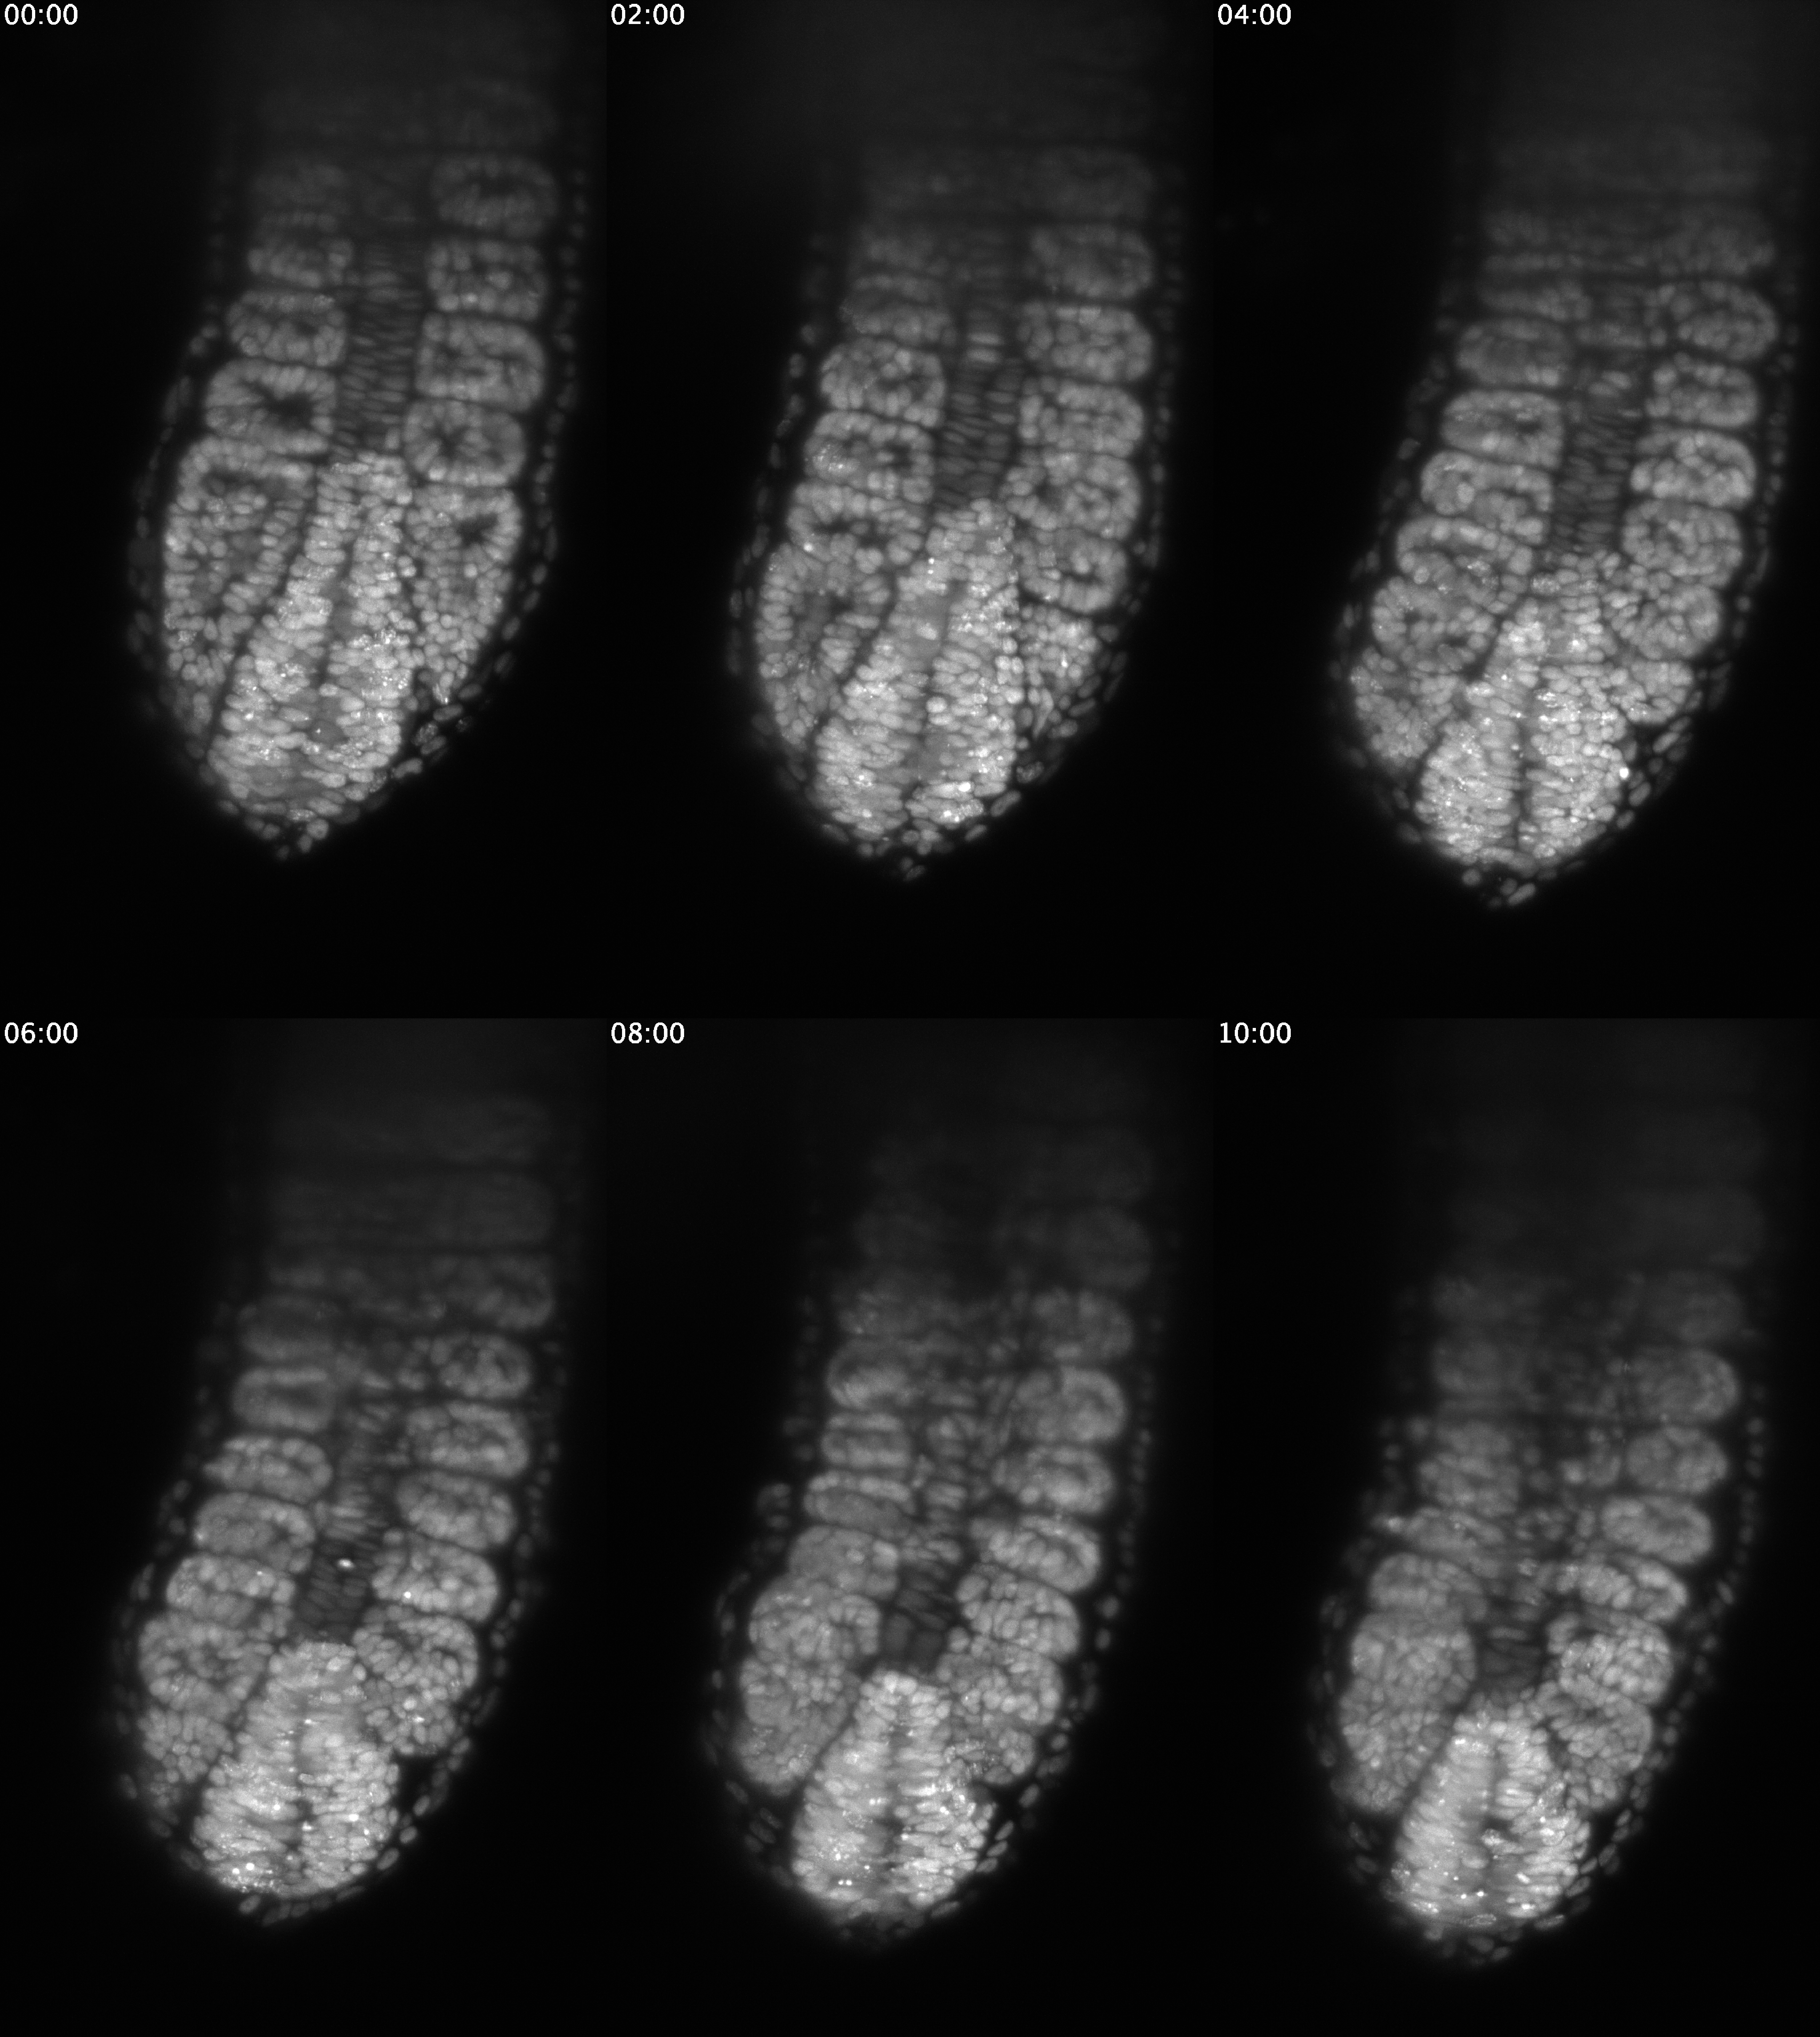
\includegraphics[width=1\linewidth]{figs/somites/ali_fish_seg_compiled} \hfill{}

\caption{Time-stamped images of somite segmentation in medaka, generated by Ali Seleit.}\label{fig:somite-seg-ali}
\end{figure}

The period of somite formation is controlled by a molecular oscillator, known as the `segmentation clock', which drives waves of gene expression in the Notch, fibroblast growth factor (FGF), and Wnt pathways, forming a signalling gradient that regresses towards the tail in concert with axis elongation (Gomez et al. 2008). Over the course of elongation, the wave period increases (i.e.~each somite takes longer to form), and the PSM progressively shrinks until it is exhausted, eventually terminating somite formation (Gomez et al. 2008).

It is not fully understood how the phase waves of the segmentation clock are initially established (Falk et al. 2022). Matsuda et al. (2020) found that period differences between mouse and human occur at the single-cell level (i.e.~not due to intercellular communication), and are driven by biochemical reaction speeds - specifically, mRNA and protein degradation rates, transcription and translation delays, and intron and splicing delays. To identify the genetic basis of these biochemical differences, our collaborators Ali Seleit and Alexander Aulehla at EMBL-Heidelberg used a CRISPR-Cas9 knock-in approach (Seleit, Aulehla, and Paix 2021) to establish a medaka \emph{Cab} strain with an endogenous, fluorescing reporter gene (Her7-Venus) for the oscillation signalling pathway. This method allows them to image somite formation and extract quantitative measures for segmentation clock dynamics, and they determined that the southern Japanese \emph{Cab} strain and the northern Japanese \emph{Kaga} strain have divergent somite periodicity, where \emph{Kaga}'s tends to be faster, and \emph{Cab}'s slower (\textbf{Figure \ref{fig:F0-Cab-Kaga-HdrR}}).



\begin{figure}

{\centering \includegraphics[width=0.5\linewidth]{figs/somites/ali_period_F0_Cab_Kaga} 

}

\caption{Comparison of period for three inbred medaka strains (\emph{Cab}, \emph{Kaga} and \emph{HdrR}). Kaga's period is lower, and therefore it takes less time to form each somite than \emph{Cab}. Figure generated by Ali Seleit.}\label{fig:F0-Cab-Kaga-HdrR}
\end{figure}

Our collaborators accordingly set up an F\textsubscript{2} cross experiment as described above, using the reporter-carrying \emph{Cab} strain and the \emph{Kaga} strain as the parental F\textsubscript{0} strains, in order to identify genetic loci associated with these differences in clock dynamics. They inter-crossed the hybrid F\textsubscript{1} generation to create a sample of 622 F\textsubscript{2} individuals, imaged the developing embryos of these F\textsubscript{2} samples, and used pyBOAT (Schmal, Mönke, and Granada 2022) to extract the oscillation features during somite development. \textbf{Figure \ref{fig:somite-period-ali}} shows a series of raw images used by pyBOAT to track the elongation of a medaka tail during somitogenesis, with the identified posterior tip of the embryo labelled with a blue circle. In \textbf{Chapter \ref{Somite-chap}}, I describe the bioinformatic analyses I performed to map the genetic variants associated with this period phenotype.



\begin{figure}

{\centering \includegraphics[width=0.8\linewidth]{figs/somites/ali_compiled_somite_elong} 

}

\caption{Screenshots of vertebral elongation in an F\textsubscript{2} individual captured by Ali Seleit during imaging. The blue circle represents the point tracked by pyBOAT over time, generating the quantitative phenotype data on period development used in this study.}\label{fig:somite-period-ali}
\end{figure}

\hypertarget{behaviour}{%
\subsection{Behaviour}\label{behaviour}}

In \textbf{Chapters \ref{Pilot-chap}} and \textbf{\ref{MIKK-F2-chap}} I use medaka as a model organism to explore social genetic effects on bold-type behaviours. Behaviour is a complex trait that is affected by both genes and environment, and for social animals such as humans and medaka, one's social environment is considered likely to constitute a large component of the environmental effect (Ruzzante and Doyle 1990; Young 2008). Apart from social aspects, an organism must face many ``hostile forces of nature'' throughout its life (Buss 1991; Darwin 1859), such as food shortages, predation, harsh climate, and diseases. Adaptive behaviours allow individuals to navigate such dangers and maximise the likelihood of their survival at both the individual and population level (Lima and Dill 1990).

Boldness-shyness is thought to be a fundamental axis of behavioural variation in many species, with an obvious causal relationship to an individual's likelihood of survival, and consequently with natural selection at the population level (Sloan Wilson et al. 1994). It represents an evolutionary trade-off between acquiring benefits (in terms of food or mates) and avoiding harms (in terms of predators or conspecific competitors), with each situation accompanied by its own optimal degree of risk (Lima and Dill 1990). It is both heritable (Svartberg 2002; Culum Brown, Burgess, and Braithwaite 2007), and subject to change following different life experiences or under different environmental conditions (Culum Brown, Burgess, and Braithwaite 2007).

This axis of behaviour has been studied extensively in many organisms. Two generic paradigms for measuring boldness include the `open field' test, and the `novel object' test. The open field test involves observing the test subject while it moves freely in an experimental setting, and has been performed on the bullfrog tadpole (Carlson and Langkilde 2013), gecko (Nordberg, Denny, and Schwarzkopf 2021), mouse (Garfield et al. 2011; Yuen et al. 2017), rat (Baud et al. 2014), rabbit (Meijsser et al. 1989), common vole (Herde and Eccard 2013), and Siberian dwarf hamster (Kanda, Louon, and Straley 2012). It is particularly favoured with fish, where the general interpretation is that shy individuals tend to react to novelty by reducing their activity and becoming more vigilant, whereas bold individuals show higher levels of activity and exploratory behaviour (C. Brown, Jones, and Braithwaite 2007; Matsunaga and Watanabe 2010; Laland, Krause, and Brown 2011; Dahlbom et al. 2011; Lucon-Xiccato and Bisazza 2017; Alfonso et al. 2019; Lucon-Xiccato et al. 2020, 2022; Hamilton et al. 2021){]}

The second paradigm is the `novel object' test, where a novel object is introduced to the test subject's environment as a way of simulating a threat. The test has been used with birds (de Azevedo and Young 2006), squirrels (Uchida et al. 2019), rabbits (A. Andersson, Laikre, and Bergvall 2014), baboons (Carter et al. 2012), vervet monkeys (Blaszczyk 2017), and grey mouse lemurs (Dammhahn and Almeling 2012). Like the open field test, it has also been extensively used with fish (C. Brown, Jones, and Braithwaite 2007; Schjolden, Stoskhus, and Winberg 2005; Wilson et al. 1993; Dominic Wright, Butlin, and Carlborg 2006; D. Wright et al. 2003; Hamilton et al. 2021).

Where both test paradigms are performed on the same fish, the behaviours exhibited were found to be correlated across assays, indicating that both were measuring the same boldness-shyness axis (C. Brown, Jones, and Braithwaite 2007). Both the open field and novel object test also permit the measurement of habituation, where the response of the fish may change over time after growing accustomed to the new environment or object. Variation in the length of time the fish take to return to a more ``normal'' level of movement may indicate different levels of boldness (Laland, Krause, and Brown 2011).

\hypertarget{SGE}{%
\subsection{Social genetic effects}\label{SGE}}

The experiments I describe in \textbf{Chapters \ref{Pilot-chap}} and \textbf{\ref{MIKK-F2-chap}} are designed to simultaneously measure both the direct effect of an individual's genes on their behaviour, as well as the indirect effect of their social partner's genes on the focal individual's behaviour, which is also an environmental factor (Baud et al. 2017). Social genetic effects have been shown to exert influence on various traits in mice including anxiety, wound healing, immune function, and body weight (Baud et al. 2017), and various traits related to development and survival in many species of livestock (Ellen et al. 2014). However, in those studies the social interactions were maintained throughout development, and it is unclear whether social genetic effects can still exert influence on adaptive behaviours during discrete, time-limited interactions.

In \textbf{Chapter \ref{Pilot-chap}} I apply a combined open field and novel object assay to determine the respective contributions of direct and social genetic effects on bold-shy behaviours in medaka fish, using 5 previously-established inbred strains. This ``pilot study'' was intended to validate the assay by ensuring that it could detect both direct and social genetic effects, and to confirm that it isn't unduly affected by confounding factors. In \textbf{Chapter \ref{MIKK-F2-chap}} I extend this analysis over the MIKK panel. I then identify the lines that diverged in both (a) their own behaviour; and (b) the level of transmission of their behaviour onto their \emph{\definecolor{iCab_424B4D}{HTML}{424B4D}\textcolor{iCab_424B4D}{iCab}} tank partner, and then use them as the parental strains in an F\textsubscript{2} cross to identify the genetic variants associated with those differences.

\hypertarget{poor-transferability-of-polygenic-scores-to-diverse-human-populations}{%
\section{Poor transferability of polygenic scores to diverse human populations}\label{poor-transferability-of-polygenic-scores-to-diverse-human-populations}}

\textbf{Chapter \ref{Fst-chap}} -- the final chapter of this thesis -- relates to the poor transferability of polygenic scores derived from GWAS results when applied to non-European populations. Humans have long sought to use genetic information to predict an individual's likely value for a given trait, in our own species and in other organisms. It is now clear that complex traits such as height, intelligence, and behaviour are highly polygenic, meaning that they are genetically influenced by hundreds or thousands of genetic variants, each exerting a small effect in one or the other direction along the trait's spectrum (Sella and Barton 2019). A richer understanding of the cumulative effect of genetic variants on any trait allows for the prediction of the value that an individual is most likely to have for that trait. Of all human traits, diseases are particularly salient; in 2018, the global healthcare industry was valued at US\$8 trillion, and predicted to increase to US\$12 trillion by 2022 ({``The \$11.9 {Trillion Global Healthcare Market}: {Key Opportunities} \& {Strategies} (2014-2022) - {ResearchAndMarkets}.com''} 2019). This strong financial imperative complements the moral imperative to reduce suffering, together driving the question of how to use genetic information to improve human health.

Recent technological developments have made it possible to sequence human genomes at scale, and it is thought that by combining detailed genetic information with with other environmental and phenotypic information (such as lifestyle or clinical factors), clinicians could move towards the practice of ``precision medicine'', where interventions could be tailored to their patients' unique risk profiles (Wray, Goddard, and Visscher 2007). The use of genetic information to predict individuals' values for a trait of interest entails the construction of metrics known as ``polygenic scores'' (\textbf{PGS}) (Lambert, Abraham, and Inouye 2019). When the trait is a disease, PGS is commonly known as polygenic risk scores (\textbf{PRS}), or genetic risk profiling, but I use the term PGS to encompass both disease and non-disease traits.

\hypertarget{pgs-and-gwas}{%
\subsection{PGS and GWAS}\label{pgs-and-gwas}}

\hypertarget{pgs}{%
\subsubsection{PGS}\label{pgs}}

PGS using genetic information alone show modest yet reliable accuracy for the prediction of complex traits (Alicia R. Martin et al. 2019): the correlations between PGS and the trait value as measured by \(R^2\) have reached 0.24 for height (Yengo et al. 2018), and 0.12-0.16 for educational attainment (Okbay et al. 2022). PGS also improve predictions beyond non-genetic clinical models for a variety of health-related traits, including breast cancer (Maas et al. 2016), prostate cancer (Schumacher et al. 2018), and type I diabetes (Sharp et al. 2019). The predictive accuracy of PGS scores can be further improved by combining genetic information with lifestyle and clinical factors, as seen with cardiovascular disease (Khera et al. 2018; Kullo et al. 2016; Natarajan et al. 2017; Paquette et al. 2017; Tikkanen et al. 2013; Sun et al. 2021).

\hypertarget{gwas}{%
\subsubsection{GWAS}\label{gwas}}

Most GWAS have been performed with individuals of European ancestry, despite only constituting around 16\% of the present global population. Although the proportion of participants in GWAS from a non-European background increased from 4\% in 2009 to 16\% in 2016 (Popejoy and Fullerton 2016)), as of 2019, 79\% of all GWAS participants recorded in the GWAS Catalog were of European ancestry, and the proportion of non-European individuals has remained the same or reduced since late 2014 (Alicia R. Martin et al. 2019). This bias extends to PGS studies, where as of 2019, only 67\% of them included only participants of European ancestry, with another 19\% including only East Asian ancestry participants, and only 3.8\% with cohorts of African, Hispanic, or Indigenous ancestry (Duncan et al. 2019).

It is therefore unsurprising that PGS scores are far better at predicting disease risk in individuals of European ancestry than in those of non-European ancestry (Alicia R. Martin et al. 2017; Alicia R. Martin et al. 2019). Indeed, the predictive accuracy of PGS scores decays with genetic divergence of the GWAS ``independent'' or ``test'' sample, from the ``discovery'' or ``training'' sample, as established in both humans (Alicia R. Martin et al. 2017; Alicia R. Martin et al. 2019), and livestock (Clark et al. 2012; Habier et al. 2010; Pszczola et al. 2012). Compared to PGS scores for those of European ancestry, PGS scores across multiple traits are \textasciitilde64-78\% less accurate for individuals of African ancestry, (Duncan et al. 2019; Alicia R. Martin et al. 2019), \textasciitilde50\% less accurate for individuals of East-Asian ancestry, and \textasciitilde37\% less accurate for individuals of South-Asian ancestry (Alicia R. Martin et al. 2019).

\hypertarget{contributors-to-pgs-non-transferability}{%
\subsection{Contributors to PGS non-transferability}\label{contributors-to-pgs-non-transferability}}

What explains this disparity in predictive value? A number of factors may be responsible, including:

\begin{enumerate}
\def\labelenumi{\arabic{enumi}.}
\item
  The failure of GWAS to identify causal variants that either do not exist or are not identifiable within the ``discovery'' sample, for both technological and methodological reasons (Alicia R. Martin et al. 2019);
\item
  The sample populations may differ in linkage disequilibrium (\textbf{LD}) -- the correlation structure of the genome -- which would change the estimated effect sizes of the causal variants, even when the causal variants themselves are the same (Alicia R. Martin et al. 2019);
\item
  Allele frequencies of the causal variants, and the distribution of the effect sizes of the causal variants, may differ between populations (Alicia R. Martin et al. 2017; Scutari, Mackay, and Balding 2016); and
\item
  The environments and demographies of populations tend to differ. Such differences are often correlated with genetic divergence due to geography, making it difficult to determine whether the associations are driven by the differences between population in their genetics, or their environments (Alicia R. Martin et al. 2019; Kerminen et al. 2019).
\end{enumerate}

The first three factors can degrade predictive performance even in the absence of biological and environmental differences. On the other hand, environmental and demographic differences can drive forces of natural selection which can in turn drive differences in causal genetic architecture (Alicia R. Martin et al. 2019).

I discuss each of these factors in turn before addressing point (3) in \textbf{Chapter \ref{Fst-chap}}.

\hypertarget{fst-discovery-sec}{%
\subsubsection{Technological and methodological limitations of GWAS}\label{fst-discovery-sec}}

The power to discover a causal variant through GWAS depends on the variant's effect size and frequency in the study population (Alicia R. Martin et al. 2019; Sham et al. 2000). That is to say, the stronger the variant's effect, or the more common it is, the more likely it is to be discovered. Rare variants tend to have stronger effect sizes (Watanabe et al. 2019), likely due to purifying selection (Park et al. 2011), and tend not to be shared across populations (Gravel et al. 2011; 1000. G. P. Consortium et al. 2015). This is particularly relevant for African populations, as they have a much greater level of genetic variance than other populations due to the human species having originated on that continent (1000. G. P. Consortium et al. 2015). Therefore, if GWAS aren't performed on diverse populations, PGS can't take into account the rare variants present in non-European populations that are likely to exert stronger effects on the trait of interest. There are also several other issues that can affect the discoverability of causal variants through GWAS, including the technology used for genotyping, the selection of the cohort, and the necessary exclusion of genotypic outliers.

With respect to genotyping technologies, GWAS often use data from SNP microarrays. These do not sequence the whole genome, but rather a selection (from several hundred thousand to millions) of genetic markers intended to present \emph{common} genetic variation (Porcu et al. 2013), which accordingly tend to neglect rare genetic variants (Uffelmann et al. 2021). To increase the density of genotypes, which would increase the likelihood of refining the association signal and identifying causal variants, researchers often ``impute'' variants that aren't sequenced directly (Porcu et al. 2013). The imputation process involves ``phasing'' the study genotypes onto the genotypes of a ``reference panel'' (McCarthy et al. 2016). However, if the reference panel does not sufficiently represent the population in the study sample, they are likely to miss or incorrectly impute those genotypes (Alicia R. Martin et al. 2019). Again, this is particularly problematic for under-represented African populations.

The lack of representation of rare variants in SNP microarrays can be overcome by using next-generation sequencing technologies such as whole-genome sequencing (\textbf{WGS}) and whole-exome sequencing (\textbf{WES}). (The former seeks to sequence the full genome, and the latter of only targets the coding regions of the genome.) These methods are more expensive than SNP microarrays, which hinders their widespread use at scale, and although their costs are continuing to decrease rapidly, there is a question as to whether they return a proportionate benefit in all use cases (Schwarze et al. 2018).

A second limitation is the selection of GWAS cohorts, which can introduce selection and collider biases (Uffelmann et al. 2021). For instance, the UK Biobank, which contains genetic and phenotypic data on 500,000 participants who volunteered for inclusion between 2006 and 2010, tend to be older, female, healthier, and wealthier than non-participants (Fry et al. 2017). This creates the possibility of confounding genetic associations with environmental factors, which I discuss further in section \ref{fst-env-sec} of Chapter \ref{Fst-chap}

A third limitation is the ``quality control'' step that is required during the GWAS process (Uffelmann et al. 2021). To avoid confounding from population stratification, which can lead to overestimated heritability and biased PGS, GWAS cohorts are filtered to include only those with similar ancestries -- or relative genetic homogeneity -- by clustering individuals through principal component analysis (\textbf{PCA}) of their genotypes, and excluding outliers. I elaborate on the issue of population stratification in section \ref{fst-env-sec} below, but at present, a statistical model for GWAS that can include cohorts with diverse ancestries without the risk of serious confounding is yet to be developed (Berg et al. 2019).

\hypertarget{differences-in-ld}{%
\subsubsection{Differences in LD}\label{differences-in-ld}}

Because GWAS SNP markers are often not the causal variants themselves, but merely in physical proximity to them, the estimated effect size of a SNP marker depends on the extent to which it is in LD with the causal variant (Mostafavi et al. 2020; Jonathan K. Pritchard and Przeworski 2001). To illustrate the problem, if a SNP has an LD \(r^2\) with a causal variant of 0.8 in the discovery population and 0.6 in the target population, it would explain 25\% = (1 - 0.6/0.8) less trait variation in the target population, and would therefore be less predictive (Ying Wang et al. 2020).

These differences in effect-size estimates may typically be small for most regions of the genome, but as PGS sum across all such effects, they aggregate these population differences (Alicia R. Martin et al. 2019; Berg et al. 2019). Previous empirical and simulation studies have shown that accuracy of PGS scores decay with increased genetic differentiation (\(F_{ST}\) -- described below in \ref{Fst-descr}) and LD differences between populations (Habier et al. 2010; Pszczola et al. 2012; Scutari, Mackay, and Balding 2016; Ying Wang et al. 2020). The issue may be addressed to a degree by using LD information from an external reference panel as a prior to infer the posterior mean effect size of a genetic variant -- Vilhjálmsson et al. (2015) demonstrated through simulations that this could improve PGS predictive accuracy. Yet the most appropriate means of deal with differences between populations in LD remains an active area of research (Duncan et al. 2019).

\hypertarget{differences-in-allele-frequencies}{%
\subsubsection{Differences in allele frequencies}\label{differences-in-allele-frequencies}}

Causal variants can differ in both frequency and effect size between different ancestry groups, e.g.~for lactase persistence (S'egurel and Bon 2017), or skin pigmentation (Adhikari et al. 2019). If a causal allele is rare in the GWAS discovery population, even if it is discovered (see section \ref{fst-discovery-sec} above), it is likely to have noisy effect size estimates, and therefore likely to inaccurately estimate its effect size in a different population where it exists at a higher frequency.

Differences in allele frequencies between populations can arise through random genetic drift, or be driven by selective pressures towards the trait optima for a given environment (Harpak and Przeworski 2021). However, evolutionary biologists have found that differences between populations in the mean values for traits tend to occur through small, coordinated shifts in their allele frequencies (Berg et al. 2019; Edge and Coop 2019). In Chapter \ref{Fst-chap}, I explore the differences in allele frequencies across populations for all polygenic traits in the GWAS Catalog, and confirm that with few exceptions -- including skin pigmentation, and HIV viral load -- the differences in allele frequencies between populations tends to be small.

\hypertarget{fst-env-sec}{%
\subsubsection{Differences in environment}\label{fst-env-sec}}

Genes continuously interact with each other (GxG, or ``epistasis'' (Gros, Le Nagard, and Tenaillon 2009)), the genes of one's parents (``genetic nurture'', Kong et al. (2018)) or social companions (``social genetic effects'') (Domingue et al. 2018; Baud et al. 2017),\footnote{Which I also explore in Chapters \ref{Pilot-chap} and \ref{MIKK-F2-chap}} and the wider non-genetic environment (GxE).

The respective contributions of genetics and environment to traits with social value -- such as intelligence -- is highly contentious, especially when there are apparent differences between populations in the mean values for those traits. PGS measure the proportion of variance within a population that is explained by genetics. Because PRS summarises a \emph{proportion} of the total variance, when studying a population that is subject to greater environmental variation, the variance attributable to genetic factors will proportionately reduce. The corollary being that when studying a population where the environment is held constant, the proportion of variance for that trait that is explained by genetic factors will approach 1. Therefore, increases in the amount of environmental variance that a population is exposed to will reduce the accuracy of PGS predictions when applied to that population.

Different environments are also often correlated with population structure (Berg et al. 2019). For example, in East Asia, there is a greater proportion of individuals of East-Asian ancestry than there is of European ancestry, and \emph{vice versa} in Europe. Those East-Asian individuals will therefore tend to share more of their genetic background with each other than with Europeans, and that population structure will be correlated with the different environments that exist in East Asia compared to Europe. This makes it difficult to determine whether it is the differences in their environments or the differences in their genetics that is driving the discrepancies between the mean values for traits between those populations. These complexities are unlikely to be resolved in the near future, which makes it attractive to turn to model organisms to address more basic biological questions regarding GxE in relation to complex traits (L. Andersson and Georges 2004), as I have done with respect to behaviour in Chapters \ref{Pilot-chap} and \ref{MIKK-F2-chap}.

\hypertarget{Fst-descr}{%
\subsection{\texorpdfstring{\(F_{ST}\)}{F\_\{ST\}}}\label{Fst-descr}}

The widely-used fixation index (\(F_{ST}\)) was introduced independently by Sewall Wright (S. Wright 1949) and Gustave Malécot (Mal'ecot 1948) as a metric for measuring the genetic diversity between populations. In Wright's notation, \(F\) refers to ``fixation'' of an allele, and \(_{ST}\) refers to ``subpopulations within the total population''. \(F_{ST}\) quantifies the relative variance in allele frequency between groups compared to within groups, reflecting the combined effects of genetic drift, migration, mutation, and selection (Holsinger and Weir 2009). The metric ranges from 0 to 1, where loci with high \(F_{ST}\) values -- that is, loci with a large relative between-group variance in allele frequencies -- may have been subject to selection or different demographic processes (Holsinger and Weir 2009). The metric has customarily been used to identify regions of the genome have been subject to diversifying selection (Akey et al. 2002; Guo, Dey, and Holsinger 2009; Weir et al. 2005).

In Chapter \ref{Fst-chap}, I extract all approximately-unlinked, trait-associated SNPs in the GWAS Catalog (MacArthur et al. 2017), and use \(F_{ST}\) to measure the differences in allele frequencies between the 26 diverse populations in the 1000 Genomes Project phase 3 release dataset (1000. G. P. Consortium et al. 2015). I then rank the traits based on the differences in the distributions of \(F_{ST}\) relative to an allele-frequency matched set of control SNPs, and find that with few exceptions (most notably, HIV viral load and race-related traits such as skin pigmentation), the diverse human populations do not differ substantially in their allele frequencies for these traits. This work provides evidence that the poor portability of PGS to non-European populations may not be attributable to differences in their allele frequencies, and may rather be attributable to differences in LD and environment.

\hypertarget{refs}{}
\begin{CSLReferences}{1}{0}
\leavevmode\vadjust pre{\hypertarget{ref-adhikariGWASLatinAmericans2019}{}}%
Adhikari, Kaustubh, Javier Mendoza-Revilla, Anood Sohail, Macarena Fuentes-Guajardo, Jodie Lampert, Juan Camilo Chac'on-Duque, Malena Hurtado, et al. 2019. {``A {GWAS} in {Latin Americans} Highlights the Convergent Evolution of Lighter Skin Pigmentation in {Eurasia}.''} \emph{Nature Communications} 10 (1, 1): 358. \url{https://doi.org/10.1038/s41467-018-08147-0}.

\leavevmode\vadjust pre{\hypertarget{ref-aidaInheritanceColorFreshWater1921}{}}%
Aida, Tatuo. 1921. {``On the {Inheritance} of {Color} in a {Fresh-Water Fish}, {Aplocheilus Latipes Temmick} and {Schlegel}, with {Special Reference} to {Sex-Linked Inheritance}.''} \emph{Genetics} 6 (6): 554--73. \url{https://www.ncbi.nlm.nih.gov/pmc/articles/PMC1200522/}.

\leavevmode\vadjust pre{\hypertarget{ref-airdBloodGroupsRelation1954}{}}%
Aird, Ian, H. H. Bentall, J. A. Mehigan, and J. A. Fraser Roberts. 1954. {``The {Blood Groups} in {Relation} to {Peptic Ulceration} and {Carcinoma} of {Colon}, {Rectum}, {Breast}, and {Bronchus}.''} \emph{Br Med J} 2 (4883): 315--21. \url{https://doi.org/10.1136/bmj.2.4883.315}.

\leavevmode\vadjust pre{\hypertarget{ref-akeyInterrogatingHighDensitySNP2002}{}}%
Akey, Joshua M., Ge Zhang, Kun Zhang, Li Jin, and Mark D. Shriver. 2002. {``Interrogating a {High-Density SNP Map} for {Signatures} of {Natural Selection}.''} \emph{Genome Research} 12 (12): 1805--14. \url{https://doi.org/10.1101/gr.631202}.

\leavevmode\vadjust pre{\hypertarget{ref-alfonsoCopingStylesEuropean2019}{}}%
Alfonso, S'ebastien, Bastien Sadoul, Manuel Gesto, Lucette Joassard, B'eatrice Chatain, Benjamin Geffroy, and Marie-Laure B'egout. 2019. {``Coping Styles in {European} Sea Bass: {The} Link Between Boldness, Stress Response and Neurogenesis.''} \emph{Physiology \& Behavior} 207 (August): 76--85. \url{https://doi.org/10.1016/j.physbeh.2019.04.020}.

\leavevmode\vadjust pre{\hypertarget{ref-allenThomasHuntMorgan1978}{}}%
Allen, Garland E. 1978. \emph{Thomas {Hunt Morgan}: {The Man} and {His Science}}. {Princeton University Press}. \url{https://books.google.com?id=MdVOAQAAIAAJ}.

\leavevmode\vadjust pre{\hypertarget{ref-altshulerGeneticMappingHuman2008}{}}%
Altshuler, David, Mark J. Daly, and Eric S. Lander. 2008. {``Genetic {Mapping} in {Human Disease}.''} \emph{Science} 322 (5903): 881--88. \url{https://doi.org/10.1126/science.1156409}.

\leavevmode\vadjust pre{\hypertarget{ref-amarasingheOpportunitiesChallengesLongread2020}{}}%
Amarasinghe, Shanika L., Shian Su, Xueyi Dong, Luke Zappia, Matthew E. Ritchie, and Quentin Gouil. 2020. {``Opportunities and Challenges in Long-Read Sequencing Data Analysis.''} \emph{Genome Biology} 21 (1): 30. \url{https://doi.org/10.1186/s13059-020-1935-5}.

\leavevmode\vadjust pre{\hypertarget{ref-anderssonTwoShadesBoldness2014}{}}%
Andersson, Anastasia, Linda Laikre, and Ulrika A. Bergvall. 2014. {``Two Shades of Boldness: Novel Object and Anti-Predator Behavior Reflect Different Personality Dimensions in Domestic Rabbits.''} \emph{Journal of Ethology} 32 (3): 123--36. \url{https://doi.org/10.1007/s10164-014-0401-9}.

\leavevmode\vadjust pre{\hypertarget{ref-anderssonDomesticanimalGenomicsDeciphering2004}{}}%
Andersson, Leif, and Michel Georges. 2004. {``Domestic-Animal Genomics: Deciphering the Genetics of Complex Traits.''} \emph{Nature Reviews Genetics} 5 (3, 3): 202--12. \url{https://doi.org/10.1038/nrg1294}.

\leavevmode\vadjust pre{\hypertarget{ref-aristotleGenerationAnimals2021}{}}%
Aristotle. 2021. \emph{On the {Generation} of {Animals}}. {Good Press}. \url{https://books.google.com?id=aLUqEAAAQBAJ}.

\leavevmode\vadjust pre{\hypertarget{ref-armstrongEnglishParsonnaturalistCompanionship2000}{}}%
Armstrong, Patrick. 2000. \emph{The {English Parson-naturalist}: {A Companionship Between Science} and {Religion}}. {Gracewing Publishing}. \url{https://books.google.com?id=hB0hEc4CN3wC}.

\leavevmode\vadjust pre{\hypertarget{ref-averyStudiesChemicalNature1944}{}}%
Avery, Oswald T., Colin M. MacLeod, and Maclyn McCarty. 1944. {``Studies on the Chemical Nature of the Substance Inducing Transformation of Pneumococcal Types: {Induction} of Transformation by a Desoxyribonucleic Acid Fraction Isolated from Pneumococcus Type {II}.''} \emph{Journal of Experimental Medicine} 79 (2): 137--58. \url{https://doi.org/10.1084/jem.79.2.137}.

\leavevmode\vadjust pre{\hypertarget{ref-bancroftPartIntroductionGouldian2016}{}}%
Bancroft, Paul. 2016. {``Part 1: {An} Introduction to the {Gouldian} Finch - {Planet Aviary}.''} February 17, 2016. \url{https://planetaviary.com/part-1-an-introduction-to-the-gouldian-finch/}.

\leavevmode\vadjust pre{\hypertarget{ref-barrettGlobalizingSocialMovement2004}{}}%
Barrett, Deborah, and Charles Kurzman. 2004. {``Globalizing Social Movement Theory: {The} Case of Eugenics.''} \emph{Theory and Society} 33 (5): 487--527. \url{https://doi.org/10.1023/B:RYSO.0000045719.45687.aa}.

\leavevmode\vadjust pre{\hypertarget{ref-barshGuidelinesGenomeWideAssociation2012}{}}%
Barsh, Gregory S., Gregory P. Copenhaver, Greg Gibson, and Scott M. Williams. 2012. {``Guidelines for {Genome-Wide Association Studies}.''} \emph{PLOS Genetics} 8 (7): e1002812. \url{https://doi.org/10.1371/journal.pgen.1002812}.

\leavevmode\vadjust pre{\hypertarget{ref-bartonSewallWrightEvolution2016}{}}%
Barton, Nicholas H. 2016. {``Sewall {Wright} on {Evolution} in {Mendelian Populations} and the {`{Shifting Balance}'}.''} \emph{Genetics} 202 (1): 3--4. \url{https://doi.org/10.1534/genetics.115.184796}.

\leavevmode\vadjust pre{\hypertarget{ref-bartovHolocaustOriginsImplementation2015}{}}%
Bartov, Omer. 2015. \emph{The {Holocaust}: {Origins}, {Implementation}, {Aftermath}}. {Routledge}. \url{https://books.google.com?id=m84JSgAACAAJ}.

\leavevmode\vadjust pre{\hypertarget{ref-bashfordOxfordHandbookHistory2010a}{}}%
Bashford, Alison, and Philippa Levine. 2010. \emph{The {Oxford Handbook} of the {History} of {Eugenics}}. {Oxford University Press, USA}. \url{https://books.google.com?id=Ml4vDwAAQBAJ}.

\leavevmode\vadjust pre{\hypertarget{ref-batesonMaterialsStudyVariation1894}{}}%
Bateson, William. 1894. \emph{Materials for the {Study} of {Variation}: {Treated} with {Especial Regard} to {Discontinuity} in the {Origin} of {Species}}. {Macmillan and Company}. \url{https://books.google.com?id=_HIZAAAAYAAJ}.

\leavevmode\vadjust pre{\hypertarget{ref-batesonMendelPrinciplesHeredity1909}{}}%
---------. 1909. {``Mendel's {Principles} of {Heredity}: {Cambridge University Press}.''} \emph{März 1909; 2nd Impr} 3: 1913.

\leavevmode\vadjust pre{\hypertarget{ref-baudGenomesPhenomesPopulation2014}{}}%
Baud, Amelie, Victor Guryev, Oliver Hummel, Martina Johannesson, and Jonathan Flint. 2014. {``Genomes and Phenomes of a Population of Outbred Rats and Its Progenitors.''} \emph{Scientific Data} 1 (1, 1): 140011. \url{https://doi.org/10.1038/sdata.2014.11}.

\leavevmode\vadjust pre{\hypertarget{ref-baudGeneticVariationSocial2017}{}}%
Baud, Amelie, Megan K. Mulligan, Francesco Paolo Casale, Jesse F. Ingels, Casey J. Bohl, Jacques Callebert, Jean-Marie Launay, et al. 2017. {``Genetic {Variation} in the {Social Environment Contributes} to {Health} and {Disease}.''} \emph{PLOS Genetics} 13 (1): e1006498. \url{https://doi.org/10.1371/journal.pgen.1006498}.

\leavevmode\vadjust pre{\hypertarget{ref-bergReducedSignalPolygenic2019}{}}%
Berg, Jeremy J, Arbel Harpak, Nasa Sinnott-Armstrong, Anja Moltke Joergensen, Hakhamanesh Mostafavi, Yair Field, Evan August Boyle, et al. 2019. {``Reduced Signal for Polygenic Adaptation of Height in {UK Biobank}.''} Edited by Magnus Nordborg, Mark I McCarthy, Magnus Nordborg, Nicholas H Barton, and Joachim Hermisson. \emph{eLife} 8 (March): e39725. \url{https://doi.org/10.7554/eLife.39725}.

\leavevmode\vadjust pre{\hypertarget{ref-bergelsonIdentifyingGenesUnderlying2010}{}}%
Bergelson, Joy, and Fabrice Roux. 2010. {``Towards Identifying Genes Underlying Ecologically Relevant Traits in {Arabidopsis} Thaliana.''} \emph{Nature Reviews Genetics} 11 (12, 12): 867--79. \url{https://doi.org/10.1038/nrg2896}.

\leavevmode\vadjust pre{\hypertarget{ref-bjorkmanSellingEugenicsCase2010}{}}%
Björkman, Maria, and Sven Widmalm. 2010. {``Selling Eugenics: The Case of {Sweden}.''} \emph{Notes and Records of the Royal Society} 64 (4): 379--400. \url{https://doi.org/10.1098/rsnr.2010.0009}.

\leavevmode\vadjust pre{\hypertarget{ref-blackWarWeakEugenics2012}{}}%
Black, Edwin. 2012. \emph{War {Against} the {Weak}: {Eugenics} and {America}'s {Campaign} to {Create} a {Master Race}, {Expanded Edition}}. {Dialog Press}. \url{https://books.google.com?id=xzwTEAAAQBAJ}.

\leavevmode\vadjust pre{\hypertarget{ref-blajStructuralVariantsTandem2022}{}}%
Blaj, Iulia, Jens Tetens, Jörn Bennewitz, Georg Thaller, and Clemens Falker-Gieske. 2022. {``Structural Variants and Tandem Repeats in the Founder Individuals of Four {F2} Pig Crosses and Implications to {F2 GWAS} Results.''} \emph{BMC Genomics} 23 (1): 631. \url{https://doi.org/10.1186/s12864-022-08716-0}.

\leavevmode\vadjust pre{\hypertarget{ref-blaszczykBoldnessNovelObjects2017}{}}%
Blaszczyk, Maryjka B. 2017. {``Boldness Towards Novel Objects Predicts Predator Inspection in Wild Vervet Monkeys.''} \emph{Animal Behaviour} 123 (January): 91--100. \url{https://doi.org/10.1016/j.anbehav.2016.10.017}.

\leavevmode\vadjust pre{\hypertarget{ref-brownCorrelationBoldnessBody2007}{}}%
Brown, C., F. Jones, and V. A. Braithwaite. 2007. {``Correlation Between Boldness and Body Mass in Natural Populations of the Poeciliid {Brachyrhaphis} Episcopi.''} \emph{Journal of Fish Biology} 71 (6): 1590--1601. \url{https://doi.org/10.1111/j.1095-8649.2007.01627.x}.

\leavevmode\vadjust pre{\hypertarget{ref-brownHeritableExperientialEffects2007}{}}%
Brown, Culum, Fiona Burgess, and Victoria A. Braithwaite. 2007. {``Heritable and Experiential Effects on Boldness in a Tropical Poeciliid.''} \emph{Behavioral Ecology and Sociobiology} 62 (2): 237--43. \url{https://doi.org/10.1007/s00265-007-0458-3}.

\leavevmode\vadjust pre{\hypertarget{ref-bushChapter11GenomeWide2012}{}}%
Bush, William S., and Jason H. Moore. 2012. {``Chapter 11: {Genome-Wide Association Studies}.''} \emph{PLOS Computational Biology} 8 (12): e1002822. \url{https://doi.org/10.1371/journal.pcbi.1002822}.

\leavevmode\vadjust pre{\hypertarget{ref-bussEvolutionaryPersonalityPsychology1991}{}}%
Buss, David M. 1991. {``Evolutionary Personality Psychology.''} \emph{Annual Review of Psychology} 42: 459--91. \url{https://doi.org/10.1146/annurev.ps.42.020191.002331}.

\leavevmode\vadjust pre{\hypertarget{ref-caballeroQuantitativeGenetics2020}{}}%
Caballero, Armando. 2020. \emph{Quantitative {Genetics}}. {Cambridge University Press}. \url{https://books.google.com?id=yOfWDwAAQBAJ}.

\leavevmode\vadjust pre{\hypertarget{ref-campbellKingJamesBible2010}{}}%
Campbell, Gordon. 2010. \emph{King {James Bible}: 400th {Anniversary Edition}}. {OUP Oxford}.

\leavevmode\vadjust pre{\hypertarget{ref-carlsonPersonalityTraitsAre2013}{}}%
Carlson, Bradley E., and Tracy Langkilde. 2013. {``Personality {Traits Are Expressed} in {Bullfrog Tadpoles} During {Open-Field Trials}.''} \emph{Journal of Herpetology} 47 (2): 378--83. \url{https://doi.org/10.1670/12-061}.

\leavevmode\vadjust pre{\hypertarget{ref-carterHowNotMeasure2012}{}}%
Carter, Alecia J., Harry H. Marshall, Robert Heinsohn, and Guy Cowlishaw. 2012. {``How Not to Measure Boldness: Novel Object and Antipredator Responses Are Not the Same in Wild Baboons.''} \emph{Animal Behaviour} 84 (3): 603--9. \url{https://doi.org/10.1016/j.anbehav.2012.06.015}.

\leavevmode\vadjust pre{\hypertarget{ref-charlesworthDarwinGenetics2009}{}}%
Charlesworth, Brian, and Deborah Charlesworth. 2009. {``Darwin and {Genetics}.''} \emph{Genetics} 183 (3): 757--66. \url{https://doi.org/10.1534/genetics.109.109991}.

\leavevmode\vadjust pre{\hypertarget{ref-charlesworthGeneticsInbreedingDepression2009}{}}%
Charlesworth, Deborah, and John H. Willis. 2009. {``The Genetics of Inbreeding Depression.''} \emph{Nature Reviews Genetics} 10 (11, 11): 783--96. \url{https://doi.org/10.1038/nrg2664}.

\leavevmode\vadjust pre{\hypertarget{ref-clarkImportanceInformationRelatives2012}{}}%
Clark, Samuel A., John M. Hickey, Hans D. Daetwyler, and Julius HJ van der Werf. 2012. {``The Importance of Information on Relatives for the Prediction of Genomic Breeding Values and the Implications for the Makeup of Reference Data Sets in Livestock Breeding Schemes.''} \emph{Genetics Selection Evolution} 44 (1): 4. \url{https://doi.org/10.1186/1297-9686-44-4}.

\leavevmode\vadjust pre{\hypertarget{ref-clarkeBasicStatisticalAnalysis2011}{}}%
Clarke, Geraldine M., Carl A. Anderson, Fredrik H. Pettersson, Lon R. Cardon, Andrew P. Morris, and Krina T. Zondervan. 2011. {``Basic Statistical Analysis in Genetic Case-Control Studies.''} \emph{Nature Protocols} 6 (2, 2): 121--33. \url{https://doi.org/10.1038/nprot.2010.182}.

\leavevmode\vadjust pre{\hypertarget{ref-cockTreasureYourExceptions2008}{}}%
Cock, Alan, and Donald R. Forsdyke. 2008. \emph{Treasure {Your Exceptions}: {The Science} and {Life} of {William Bateson}}. {Springer Science \& Business Media}. \url{https://books.google.com?id=FDUi1xg26gsC}.

\leavevmode\vadjust pre{\hypertarget{ref-collinsVariationsThemeCataloging1997}{}}%
Collins, Francis S., Mark S. Guyer, and Aravinda Chakravarti. 1997. {``Variations on a {Theme}: {Cataloging Human DNA Sequence Variation}.''} \emph{Science} 278 (5343): 1580--81. \url{https://doi.org/10.1126/science.278.5343.1580}.

\leavevmode\vadjust pre{\hypertarget{ref-10002015global}{}}%
Consortium, 1000 Genomes Project et al. 2015. {``A Global Reference for Human Genetic Variation.''} \emph{Nature} 526 (7571): 68.

\leavevmode\vadjust pre{\hypertarget{ref-internationalhumangenomesequencingconsortiumInitialSequencingAnalysis2001a}{}}%
Consortium, International Human Genome Sequencing. 2001. {``Initial Sequencing and Analysis of the Human Genome.''} \emph{Nature} 409 (6822, 6822): 860--921. \url{https://doi.org/10.1038/35057062}.

\leavevmode\vadjust pre{\hypertarget{ref-internationalhumangenomesequencingconsortiumInternationalConsortiumCompletes2003}{}}%
---------. 2003. {``International {Consortium Completes Human Genome Project}.''} {Genome.gov}. April 14, 2003. \url{https://www.genome.gov/11006929/2003-release-international-consortium-completes-hgp}.

\leavevmode\vadjust pre{\hypertarget{ref-coyneTheodosiusDobzhanskyHybrid2016}{}}%
Coyne, Jerry A. 2016. {``Theodosius {Dobzhansky} on {Hybrid Sterility} and {Speciation}.''} \emph{Genetics} 202 (1): 5--7. \url{https://doi.org/10.1534/genetics.115.184770}.

\leavevmode\vadjust pre{\hypertarget{ref-dahlbomBoldnessPredictsSocial2011}{}}%
Dahlbom, S. Josefin, David Lagman, Katrin Lundstedt-Enkel, L. Fredrik Sundström, and Svante Winberg. 2011. {``Boldness {Predicts Social Status} in {Zebrafish} ({Danio} Rerio).''} \emph{PLOS ONE} 6 (8): e23565. \url{https://doi.org/10.1371/journal.pone.0023565}.

\leavevmode\vadjust pre{\hypertarget{ref-dammhahnRiskTakingForaging2012}{}}%
Dammhahn, Melanie, and Laura Almeling. 2012. {``Is Risk Taking During Foraging a Personality Trait? {A} Field Test for Cross-Context Consistency in Boldness.''} \emph{Animal Behaviour} 84 (5): 1131--39. \url{https://doi.org/10.1016/j.anbehav.2012.08.014}.

\leavevmode\vadjust pre{\hypertarget{ref-darwinJournalResearchesNatural1845}{}}%
Darwin, Charles. 1845. \emph{Journal of {Researches Into} the {Natural History} and {Geology} of the {Countries Visited During} the {Voyage} of {H}.{M}.{S}. {Beagle Round} the {World}: {Under} the {Command} of {Capt}. {Fitz Roy}, {R}.{N}}. 2nd ed. {J. Murray}. \url{https://books.google.com?id=nXm9vEpV8BAC}.

\leavevmode\vadjust pre{\hypertarget{ref-darwinOriginSpeciesMeans1859}{}}%
---------. 1859. \emph{On the {Origin} of {Species} by {Means} of {Natural Selection}, {Or}, {The Preservation} of {Favoured Races} in the {Struggle} for {Life}}. {J. Murray}. \url{https://books.google.com?id=gGUYt2PsDJcC}.

\leavevmode\vadjust pre{\hypertarget{ref-darwinNaturalistVoyageJournal1882}{}}%
---------. 1882. \emph{A {Naturalist}'s {Voyage}: {Journal} of {Researches Into} the {Natural History} and {Geology} of the {Countries Visited During} the {Voyage} of {H}.{M}.{S}. {Beagle} : With {Maps} and {Illustrations}}. {Murray}. \url{https://books.google.com?id=JyR7HY3FMtkC}.

\leavevmode\vadjust pre{\hypertarget{ref-darwinLifeLettersCharles1887}{}}%
---------. 1887. \emph{The {Life} and {Letters} of {Charles Darwin}: {Including} an {Autobiographical Chapter}}. {D. Appleton}. \url{https://books.google.com?id=iodTqIRzVukC}.

\leavevmode\vadjust pre{\hypertarget{ref-darwinCharlesDarwinLetters1998}{}}%
---------. 1998. \emph{Charles {Darwin}'s {Letters}: {A Selection}, 1825-1859}. {Cambridge University Press}. \url{https://books.google.com?id=E2TTcP6KUHgC}.

\leavevmode\vadjust pre{\hypertarget{ref-darwinAutobiographyCharlesDarwin2019}{}}%
---------. 2019. \emph{The {Autobiography} of {Charles Darwin}}. {BoD -- Books on Demand}. \url{https://books.google.com?id=t_SxDwAAQBAJ}.

\leavevmode\vadjust pre{\hypertarget{ref-darwinCorrespondenceCharlesDarwin2002}{}}%
Darwin, Charles, Duncan M. Porter, Sheila Ann Dean, Samantha Evans, Shelley Innes, and Alison M. Pearn. 2002. \emph{The {Correspondence} of {Charles Darwin}: 1821-1860}. {Cambridge University Press}. \url{https://books.google.com?id=oCWGX18UrhEC}.

\leavevmode\vadjust pre{\hypertarget{ref-azevedoShynessBoldnessGreater2006}{}}%
de Azevedo, Cristiano S., and Robert J. Young. 2006. {``Shyness and Boldness in Greater Rheas {Rhea} Americana {Linnaeus} ({Rheiformes}, {Rheidae}): The Effects of Antipredator Training on the Personality of the Birds.''} \emph{Revista Brasileira de Zoologia} 23 (March): 202--10. \url{https://doi.org/10.1590/S0101-81752006000100012}.

\leavevmode\vadjust pre{\hypertarget{ref-vriesMutationTheory19091909}{}}%
de Vries, Hugo. 1909. \emph{The {Mutation} Theory v. 1, 1909}. {Open Court Publishing Company}. \url{https://books.google.com?id=cdOhB5p3HkIC}.

\leavevmode\vadjust pre{\hypertarget{ref-dirienzoPopulationGeneticsModels2006}{}}%
Di Rienzo, Anna. 2006. {``Population Genetics Models of Common Diseases.''} \emph{Current Opinion in Genetics \& Development}, Genomes and evolution, 16 (6): 630--36. \url{https://doi.org/10.1016/j.gde.2006.10.002}.

\leavevmode\vadjust pre{\hypertarget{ref-dobzhanskyGeneticsNaturalPopulations1943}{}}%
Dobzhansky, Th. 1943. {``Genetics of Natural Populations {IX}. {Temporal} Changes in the Composition of Populations of Drosophila Pseudoobscura.''} \emph{Genetics} 28 (2): 162--86. \url{https://doi.org/10.1093/genetics/28.2.162}.

\leavevmode\vadjust pre{\hypertarget{ref-domingueSocialGenomeFriends2018}{}}%
Domingue, Benjamin W., Daniel W. Belsky, Jason M. Fletcher, Dalton Conley, Jason D. Boardman, and Kathleen Mullan Harris. 2018. {``The Social Genome of Friends and Schoolmates in the {National Longitudinal Study} of {Adolescent} to {Adult Health}.''} \emph{Proceedings of the National Academy of Sciences} 115 (4): 702--7. \url{https://doi.org/10.1073/pnas.1711803115}.

\leavevmode\vadjust pre{\hypertarget{ref-drueryExperimentsPlantHybridization1901}{}}%
Druery, C. T., and William Bateson. 1901. {``Experiments in Plant Hybridization.''} \emph{Journal of the Royal Horticultural Society} 26: 1--32.

\leavevmode\vadjust pre{\hypertarget{ref-duncanAnalysisPolygenicRisk2019}{}}%
Duncan, L., H. Shen, B. Gelaye, J. Meijsen, K. Ressler, M. Feldman, R. Peterson, and B. Domingue. 2019. {``Analysis of Polygenic Risk Score Usage and Performance in Diverse Human Populations.''} \emph{Nature Communications} 10 (1, 1): 3328. \url{https://doi.org/10.1038/s41467-019-11112-0}.

\leavevmode\vadjust pre{\hypertarget{ref-dunnShortHistoryGenetics1991}{}}%
Dunn, Leslie Clarence. 1991. \emph{A {Short History} of {Genetics}: {The Development} of {Some} of the {Main Lines} of {Thought}, 1864-1939}. {Iowa State University Press}. \url{https://books.google.com?id=MpEiAQAAMAAJ}.

\leavevmode\vadjust pre{\hypertarget{ref-eatonQuartercenturyInbreedingGuineapigs1932}{}}%
Eaton, Orson N. 1932. {``A Quarter-Century of Inbreeding in Guinea-Pigs.''} \emph{Journal of Experimental Zoology} 63 (2): 261--90. \url{https://doi.org/10.1002/jez.1400630202}.

\leavevmode\vadjust pre{\hypertarget{ref-edgeReconstructingHistoryPolygenic2019}{}}%
Edge, Michael D, and Graham Coop. 2019. {``Reconstructing the {History} of {Polygenic Scores Using Coalescent Trees}.''} \emph{Genetics} 211 (1): 235--62. \url{https://doi.org/10.1534/genetics.118.301687}.

\leavevmode\vadjust pre{\hypertarget{ref-ellenProspectsSelectionSocial2014}{}}%
Ellen, Esther D., T. Bas Rodenburg, Gerard A. A. Albers, J. Elizabeth Bolhuis, Irene Camerlink, Naomi Duijvesteijn, Egbert F. Knol, et al. 2014. {``The Prospects of Selection for Social Genetic Effects to Improve Welfare and Productivity in Livestock.''} \emph{Frontiers in Genetics} 5. \url{https://www.frontiersin.org/articles/10.3389/fgene.2014.00377}.

\leavevmode\vadjust pre{\hypertarget{ref-evansQTLGeneElegans2021}{}}%
Evans, Kathryn S., Marijke H. van Wijk, Patrick T. McGrath, Erik C. Andersen, and Mark G. Sterken. 2021. {``From {QTL} to Gene: {C}. Elegans Facilitates Discoveries of the Genetic Mechanisms Underlying Natural Variation.''} \emph{Trends in Genetics} 37 (10): 933--47. \url{https://doi.org/10.1016/j.tig.2021.06.005}.

\leavevmode\vadjust pre{\hypertarget{ref-ewensTransmissionDisequilibriumTest1995}{}}%
Ewens, W J, and R S Spielman. 1995. {``The Transmission/Disequilibrium Test: History, Subdivision, and Admixture.''} \emph{American Journal of Human Genetics} 57 (2): 455--64. \url{https://www.ncbi.nlm.nih.gov/pmc/articles/PMC1801556/}.

\leavevmode\vadjust pre{\hypertarget{ref-fairbanksRelicsEdenPowerful2009}{}}%
Fairbanks, Daniel J. 2009. \emph{Relics of {Eden}: {The Powerful Evidence} of {Evolution} in {Human DNA}}. {Prometheus Books}. \url{https://books.google.com?id=O1mFjWzznWkC}.

\leavevmode\vadjust pre{\hypertarget{ref-falconerIntroductionQuantitativeGenetics1996}{}}%
Falconer, D. S., and T. F. C. Mackay. 1996. \emph{Introduction to Quantitative Genetics}. {UK: Longman Group}.

\leavevmode\vadjust pre{\hypertarget{ref-falkImagingOnsetOscillatory2022}{}}%
Falk, Henning J, Takehito Tomita, Gregor Mönke, Katie McDole, and Alexander Aulehla. 2022. {``Imaging the Onset of Oscillatory Signaling Dynamics During Mouse Embryo Gastrulation.''} \emph{Development (Cambridge, England)} 149 (13): dev200083. \url{https://doi.org/10.1242/dev.200083}.

\leavevmode\vadjust pre{\hypertarget{ref-falker-gieskeGWASMeatCarcass2019}{}}%
Falker-Gieske, Clemens, Iulia Blaj, Siegfried Preuß, Jörn Bennewitz, Georg Thaller, and Jens Tetens. 2019. {``{GWAS} for {Meat} and {Carcass Traits Using Imputed Sequence Level Genotypes} in {Pooled F2-Designs} in {Pigs}.''} \emph{G3 Genes\textbar Genomes\textbar Genetics} 9 (9): 2823--34. \url{https://doi.org/10.1534/g3.119.400452}.

\leavevmode\vadjust pre{\hypertarget{ref-fisherXVCorrelationRelatives1919}{}}%
Fisher, R. A. 1919. {``{XV}.---{The Correlation} Between {Relatives} on the {Supposition} of {Mendelian Inheritance}.''} January. \url{https://doi.org/10.1017/s0080456800012163}.

\leavevmode\vadjust pre{\hypertarget{ref-fisherProbableErrorCoefficient1921}{}}%
Fisher, Ronald Aylmer. 1921. {``On the{"} {Probable Error}{"} of a {Coefficient} of {Correlation Deduced} from a {Small Sample}.''}

\leavevmode\vadjust pre{\hypertarget{ref-fisherStatisticalMethodsResearch1925}{}}%
---------. 1925. \emph{Statistical {Methods} for {Research Workers}}. {Oliver and Boyd}. \url{https://books.google.com?id=1NApzwEACAAJ}.

\leavevmode\vadjust pre{\hypertarget{ref-fitzgeraldMedakaInbredKiyosuKarlsruhe2022}{}}%
Fitzgerald, Tomas, Ian Brettell, Adrien Leger, Nadeshda Wolf, Natalja Kusminski, Jack Monahan, Carl Barton, et al. 2022. {``The {Medaka Inbred Kiyosu-Karlsruhe} ({MIKK}) Panel.''} \emph{Genome Biology} 23 (1): 59. \url{https://doi.org/10.1186/s13059-022-02623-z}.

\leavevmode\vadjust pre{\hypertarget{ref-franklinMolecularConfigurationSodium1953}{}}%
Franklin, Rosalind E., and Raymond G. Gosling. 1953. {``Molecular Configuration in Sodium Thymonucleate.''} \emph{Nature} 171 (4356): 740--41.

\leavevmode\vadjust pre{\hypertarget{ref-fryComparisonSociodemographicHealthRelated2017}{}}%
Fry, Anna, Thomas J Littlejohns, Cathie Sudlow, Nicola Doherty, Ligia Adamska, Tim Sprosen, Rory Collins, and Naomi E Allen. 2017. {``Comparison of {Sociodemographic} and {Health-Related Characteristics} of {UK Biobank Participants With Those} of the {General Population}.''} \emph{American Journal of Epidemiology} 186 (9): 1026--34. \url{https://doi.org/10.1093/aje/kwx246}.

\leavevmode\vadjust pre{\hypertarget{ref-fukamachi100YearsMedaka2021}{}}%
Fukamachi, Shoji, and Kiyoshi Naruse. 2021. {``100 Years Since the Medaka's International Debut: {Aida}'s Legacy.''} {Genes to Genomes}. August 20, 2021. \url{https://genestogenomes.org/100-years-since-the-medakas-international-debut-aidas-legacy/}.

\leavevmode\vadjust pre{\hypertarget{ref-galtonMenScienceTheir1874a}{}}%
Galton, Francis. 1874. {``On {Men} of {Science}, Their {Nature} and Their {Nurture}.''} In \emph{Proceedings of the {Royal Institution} of {Great Britain}}, 7:227--36.

\leavevmode\vadjust pre{\hypertarget{ref-galtonInquiriesHumanFaculty1883}{}}%
---------. 1883. \emph{Inquiries {Into Human Faculty} and {Its Development}}. {Macmillan}. \url{https://books.google.com?id=GGAZAAAAYAAJ}.

\leavevmode\vadjust pre{\hypertarget{ref-galtonRegressionMediocrityHereditary1886}{}}%
---------. 1886. {``Regression {Towards Mediocrity} in {Hereditary Stature}.''} \emph{The Journal of the Anthropological Institute of Great Britain and Ireland} 15: 246--63. \url{https://doi.org/10.2307/2841583}.

\leavevmode\vadjust pre{\hypertarget{ref-galtonNaturalInheritance1889}{}}%
---------. 1889. \emph{Natural Inheritance}. {Macmillan and Company}.

\leavevmode\vadjust pre{\hypertarget{ref-galtonEugenicsItsDefinition1904}{}}%
---------. 1904. {``Eugenics: {Its Definition}, {Scope}, and {Aims}.''} \emph{American Journal of Sociology} 10 (1): 1--25. \url{https://doi.org/10.1086/211280}.

\leavevmode\vadjust pre{\hypertarget{ref-garciadeleanizGeneticDeterminationContribution1989}{}}%
Garcia de Le'aniz, C., E. Verspoor, and A. D. Hawkins. 1989. {``Genetic Determination of the Contribution of Stocked and Wild {Atlantic} Salmon, {Salmo} Salar {L}., To the Angling Fisheries in Two {Spanish} Rivers.''} \emph{Journal of Fish Biology} 35: 261--70. \url{https://doi.org/10.1111/j.1095-8649.1989.tb03069.x}.

\leavevmode\vadjust pre{\hypertarget{ref-garfieldDistinctPhysiologicalBehavioural2011}{}}%
Garfield, Alastair S., Michael Cowley, Florentia M. Smith, Kim Moorwood, Joanne E. Stewart-Cox, Kerry Gilroy, Sian Baker, et al. 2011. {``Distinct Physiological and Behavioural Functions for Parental Alleles of Imprinted {Grb10}.''} \emph{Nature} 469 (7331, 7331): 534--38. \url{https://doi.org/10.1038/nature09651}.

\leavevmode\vadjust pre{\hypertarget{ref-gomezControlSegmentNumber2008}{}}%
Gomez, C'eline, Ertuğrul M. Özbudak, Joshua Wunderlich, Diana Baumann, Julian Lewis, and Olivier Pourqui'e. 2008. {``Control of Segment Number in Vertebrate Embryos.''} \emph{Nature} 454 (7202, 7202): 335--39. \url{https://doi.org/10.1038/nature07020}.

\leavevmode\vadjust pre{\hypertarget{ref-goodnightSewallWrightSeven2014}{}}%
Goodnight, Charles. 2014. {``Sewall {Wright}'s {Seven Generalizations} about {Populations}.''} {Evolution in Structured Populations}. May 22, 2014. \url{https://blog.uvm.edu/cgoodnig/2014/05/22/sewall-wrights-seven-generalizations-about-populations/}.

\leavevmode\vadjust pre{\hypertarget{ref-gornerAlteredFatesGenetic1996}{}}%
Gorner, Peter, and Jeff Lyon. 1996. \emph{Altered {Fates}: {The Genetic Re-Engineering} of {Human Life}}. {W. W. Norton, Incorporated}. \url{https://books.google.com?id=MrhEzwEACAAJ}.

\leavevmode\vadjust pre{\hypertarget{ref-gravel2011demographic}{}}%
Gravel, Simon, Brenna M Henn, Ryan N Gutenkunst, Amit R Indap, Gabor T Marth, Andrew G Clark, Fuli Yu, et al. 2011. {``Demographic History and Rare Allele Sharing Among Human Populations.''} \emph{Proceedings of the National Academy of Sciences} 108 (29): 11983--88. \url{https://doi.org/10.1073/pnas.1019276108}.

\leavevmode\vadjust pre{\hypertarget{ref-gridleyLongShortIt2006}{}}%
Gridley, Thomas. 2006. {``The Long and Short of It: {Somite} Formation in Mice.''} \emph{Developmental Dynamics} 235 (9): 2330--36. \url{https://doi.org/10.1002/dvdy.20850}.

\leavevmode\vadjust pre{\hypertarget{ref-grosEvolutionEpistasisIts2009}{}}%
Gros, Pierre-Alexis, Herv'e Le Nagard, and Olivier Tenaillon. 2009. {``The {Evolution} of {Epistasis} and {Its Links With Genetic Robustness}, {Complexity} and {Drift} in a {Phenotypic Model} of {Adaptation}.''} \emph{Genetics} 182 (1): 277--93. \url{https://doi.org/10.1534/genetics.108.099127}.

\leavevmode\vadjust pre{\hypertarget{ref-guGenomeWideAssociationStudy2011}{}}%
Gu, Xiaorong, Chungang Feng, Li Ma, Chi Song, Yanqiang Wang, Yang Da, Huifang Li, et al. 2011. {``Genome-{Wide Association Study} of {Body Weight} in {Chicken F2 Resource Population}.''} \emph{PLOS ONE} 6 (7): e21872. \url{https://doi.org/10.1371/journal.pone.0021872}.

\leavevmode\vadjust pre{\hypertarget{ref-guoBayesianHierarchicalModel2009}{}}%
Guo, Feng, Dipak K. Dey, and Kent E. Holsinger. 2009. {``A {Bayesian Hierarchical Model} for {Analysis} of {Single-Nucleotide Polymorphisms Diversity} in {Multilocus}, {Multipopulation Samples}.''} \emph{Journal of the American Statistical Association} 104 (485): 142--54. \url{https://doi.org/10.1198/jasa.2009.0010}.

\leavevmode\vadjust pre{\hypertarget{ref-gusellaPolymorphicDNAMarker1983}{}}%
Gusella, James F., Nancy S. Wexler, P. Michael Conneally, Susan L. Naylor, Mary Anne Anderson, Rudolph E. Tanzi, Paul C. Watkins, et al. 1983. {``A Polymorphic {DNA} Marker Genetically Linked to {Huntington}'s Disease.''} \emph{Nature} 306 (5940, 5940): 234--38. \url{https://doi.org/10.1038/306234a0}.

\leavevmode\vadjust pre{\hypertarget{ref-habierImpactGeneticRelationship2010}{}}%
Habier, David, Jens Tetens, Franz-Reinhold Seefried, Peter Lichtner, and Georg Thaller. 2010. {``The Impact of Genetic Relationship Information on Genomic Breeding Values in {German Holstein} Cattle.''} \emph{Genetics Selection Evolution} 42 (1): 5. \url{https://doi.org/10.1186/1297-9686-42-5}.

\leavevmode\vadjust pre{\hypertarget{ref-hamiltonShoalingBoldnessAnxietylike2021}{}}%
Hamilton, Trevor J., Jeffrey Krook, Joshua Szaszkiewicz, and Warren Burggren. 2021. {``Shoaling, Boldness, Anxiety-Like Behavior and Locomotion in Zebrafish ({Danio} Rerio) Are Altered by Acute Benzo{[}a{]}pyrene Exposure.''} \emph{Science of The Total Environment} 774 (June): 145702. \url{https://doi.org/10.1016/j.scitotenv.2021.145702}.

\leavevmode\vadjust pre{\hypertarget{ref-hardenGeneticLotteryWhy2021}{}}%
Harden, Kathryn Paige. 2021. \emph{The {Genetic Lottery}: {Why DNA Matters} for {Social Equality}}. {Princeton University Press}. \url{https://books.google.com?id=R9oiEAAAQBAJ}.

\leavevmode\vadjust pre{\hypertarget{ref-harpakEvolutionGroupDifferences2021}{}}%
Harpak, Arbel, and Molly Przeworski. 2021. {``The Evolution of Group Differences in Changing Environments.''} \emph{PLOS Biology} 19 (1): e3001072. \url{https://doi.org/10.1371/journal.pbio.3001072}.

\leavevmode\vadjust pre{\hypertarget{ref-hartsoekerEssayDioptrique1694}{}}%
Hartsoeker, Nicolas. 1694. \emph{Essay de dioptrique}. {J. Anisson}. \url{https://books.google.com?id=IzYVAAAAQAAJ}.

\leavevmode\vadjust pre{\hypertarget{ref-hawkinsSocialDarwinismEuropean1997}{}}%
Hawkins, Mike. 1997. \emph{Social darwinism in European and American thought, 1860-1945: nature as model and nature as threat}. {Cambridge University Press}. \url{https://books.google.com?id=aoXJoAEACAAJ}.

\leavevmode\vadjust pre{\hypertarget{ref-henigMonkGardenLost2000}{}}%
Henig, Robin Marantz. 2000. \emph{The {Monk} in the {Garden}: {The Lost} and {Found Genius} of {Gregor Mendel}, the {Father} of {Genetics}}. {Houghton Mifflin Harcourt}.

\leavevmode\vadjust pre{\hypertarget{ref-henslowLetter1051831}{}}%
Henslow, John. 1831. {``Letter 105.''} {Darwin Correspondence Project}. 1831. \url{https://www.darwinproject.ac.uk/letter/DCP-LETT-105.xml}.

\leavevmode\vadjust pre{\hypertarget{ref-herdeConsistencyBoldnessActivity2013}{}}%
Herde, Antje, and Jana A. Eccard. 2013. {``Consistency in Boldness, Activity and Exploration at Different Stages of Life.''} \emph{BMC Ecology} 13 (1): 49. \url{https://doi.org/10.1186/1472-6785-13-49}.

\leavevmode\vadjust pre{\hypertarget{ref-hillDataTheoryPoint2008}{}}%
Hill, William G., Michael E. Goddard, and Peter M. Visscher. 2008. {``Data and {Theory Point} to {Mainly Additive Genetic Variance} for {Complex Traits}.''} \emph{PLOS Genetics} 4 (2): e1000008. \url{https://doi.org/10.1371/journal.pgen.1000008}.

\leavevmode\vadjust pre{\hypertarget{ref-hochbergMorePowerfulProcedures1990}{}}%
Hochberg, Yosef, and Yoav Benjamini. 1990. {``More Powerful Procedures for Multiple Significance Testing.''} \emph{Statistics in Medicine} 9 (7): 811--18. \url{https://doi.org/10.1002/sim.4780090710}.

\leavevmode\vadjust pre{\hypertarget{ref-hodgeGeneticEngineeringManipulating2009}{}}%
Hodge, Russ. 2009. \emph{Genetic {Engineering}: {Manipulating} the {Mechanisms} of {Life}}. {Infobase Publishing}. \url{https://books.google.com?id=Fqa6lmQ_YVMC}.

\leavevmode\vadjust pre{\hypertarget{ref-holsingerGeneticsGeographicallyStructured2009}{}}%
Holsinger, Kent E., and Bruce S. Weir. 2009. {``Genetics in Geographically Structured Populations: Defining, Estimating and Interpreting {FST}.''} \emph{Nature Reviews Genetics} 10 (9, 9): 639--50. \url{https://doi.org/10.1038/nrg2611}.

\leavevmode\vadjust pre{\hypertarget{ref-hubaudSignallingDynamicsVertebrate2014}{}}%
Hubaud, Alexis, and Olivier Pourqui'e. 2014. {``Signalling Dynamics in Vertebrate Segmentation.''} \emph{Nature Reviews Molecular Cell Biology} 15 (11, 11): 709--21. \url{https://doi.org/10.1038/nrm3891}.

\leavevmode\vadjust pre{\hypertarget{ref-huxleyEvolutionModernSynthesis1942}{}}%
Huxley, Julian. 1942. {``Evolution. {The} Modern Synthesis.''} \emph{Evolution. The Modern Synthesis.}

\leavevmode\vadjust pre{\hypertarget{ref-iselyOneHundredOne2002}{}}%
Isely, Duane. 2002. \emph{One {Hundred} and {One Botanists}}. {Purdue University Press}. \url{https://books.google.com?id=an6r8m0JfV8C}.

\leavevmode\vadjust pre{\hypertarget{ref-jainNanoporeSequencingAssembly2018}{}}%
Jain, Miten, Sergey Koren, Karen H. Miga, Josh Quick, Arthur C. Rand, Thomas A. Sasani, John R. Tyson, et al. 2018. {``Nanopore Sequencing and Assembly of a Human Genome with Ultra-Long Reads.''} \emph{Nature Biotechnology} 36 (4, 4): 338--45. \url{https://doi.org/10.1038/nbt.4060}.

\leavevmode\vadjust pre{\hypertarget{ref-jenkinOriginSpecies1867}{}}%
Jenkin, Fleeming. 1867. {``The Origin of Species.''} \emph{North British Review} 46 (92): 277--318.

\leavevmode\vadjust pre{\hypertarget{ref-johnsonSegregationPerformanceRecombinant1999}{}}%
Johnson, William C., and Paul Gepts. 1999. {``Segregation for Performance in Recombinant Inbred Populations Resulting from Inter-Gene Pool Crosses of Common Bean ( {Phaseolus} Vulgaris {L}.).''} \emph{Euphytica} 106 (1): 45--56. \url{https://doi.org/10.1023/A:1003541201923}.

\leavevmode\vadjust pre{\hypertarget{ref-kandaStabilityActivityBoldness2012}{}}%
Kanda, L. Leann, Laura Louon, and Katherine Straley. 2012. {``Stability in {Activity} and {Boldness Across Time} and {Context} in {Captive Siberian Dwarf Hamsters}.''} \emph{Ethology} 118 (6): 518--33. \url{https://doi.org/10.1111/j.1439-0310.2012.02038.x}.

\leavevmode\vadjust pre{\hypertarget{ref-karlNationalLifeStandpoint1901a}{}}%
Karl, Pearson. 1901. \emph{National {Life} from the Standpoint of {Science}}. {London}.

\leavevmode\vadjust pre{\hypertarget{ref-kenneyThomasHuntMorgan2009}{}}%
Kenney, Diana E, and Gary G Borisy. 2009. {``Thomas {Hunt Morgan} at the {Marine Biological Laboratory}: {Naturalist} and {Experimentalist}.''} \emph{Genetics} 181 (3): 841--46. \url{https://doi.org/10.1534/genetics.109.101659}.

\leavevmode\vadjust pre{\hypertarget{ref-kerminenGeographicVariationBias2019}{}}%
Kerminen, Sini, Alicia R. Martin, Jukka Koskela, Sanni E. Ruotsalainen, Aki S. Havulinna, Ida Surakka, Aarno Palotie, et al. 2019. {``Geographic {Variation} and {Bias} in the {Polygenic Scores} of {Complex Diseases} and {Traits} in {Finland}.''} \emph{The American Journal of Human Genetics} 104 (6): 1169--81. \url{https://doi.org/10.1016/j.ajhg.2019.05.001}.

\leavevmode\vadjust pre{\hypertarget{ref-kevlesNameEugenicsGenetics1995}{}}%
Kevles, Daniel J. 1995. \emph{In the {Name} of {Eugenics}: {Genetics} and the {Uses} of {Human Heredity}}. {Harvard University Press}. \url{https://books.google.com?id=NWBi9kyb8xUC}.

\leavevmode\vadjust pre{\hypertarget{ref-kheraGenomewidePolygenicScores2018}{}}%
Khera, Amit V., Mark Chaffin, Krishna G. Aragam, Mary E. Haas, Carolina Roselli, Seung Hoan Choi, Pradeep Natarajan, et al. 2018. {``Genome-Wide Polygenic Scores for Common Diseases Identify Individuals with Risk Equivalent to Monogenic Mutations.''} \emph{Nature Genetics} 50 (9, 9): 1219--24. \url{https://doi.org/10.1038/s41588-018-0183-z}.

\leavevmode\vadjust pre{\hypertarget{ref-kimPeriodSomiteSegmentation2011}{}}%
Kim, Woong, Takaaki Matsui, Masataka Yamao, Makoto Ishibashi, Kota Tamada, Toru Takumi, Kenji Kohno, et al. 2011. {``The Period of the Somite Segmentation Clock Is Sensitive to {Notch} Activity.''} \emph{Molecular Biology of the Cell} 22 (18): 3541--49. \url{https://doi.org/10.1091/mbc.e11-02-0139}.

\leavevmode\vadjust pre{\hypertarget{ref-kleinHLASystem2000}{}}%
Klein, Jan, and Akie Sato. 2000. {``The {HLA System}.''} \emph{New England Journal of Medicine} 343 (11): 782--86. \url{https://doi.org/10.1056/NEJM200009143431106}.

\leavevmode\vadjust pre{\hypertarget{ref-knopikBehavioralGenetics2019}{}}%
Knopik, Valerie S., Jenae M. Neiderhiser, John C. DeFries, and Robert Plomin. 2019. \emph{Behavioral {Genetics}}. {Macmillan Learning}. \url{https://books.google.com?id=mtDJvQEACAAJ}.

\leavevmode\vadjust pre{\hypertarget{ref-kongNatureNurtureEffects2018}{}}%
Kong, Augustine, Gudmar Thorleifsson, Michael L. Frigge, Bjarni J. Vilhjalmsson, Alexander I. Young, Thorgeir E. Thorgeirsson, Stefania Benonisdottir, et al. 2018. {``The Nature of Nurture: {Effects} of Parental Genotypes.''} \emph{Science} 359 (6374): 424--28. \url{https://doi.org/10.1126/science.aan6877}.

\leavevmode\vadjust pre{\hypertarget{ref-kulloIncorporatingGeneticRisk2016}{}}%
Kullo, Iftikhar J., Hayan Jouni, Erin E. Austin, Sherry-Ann Brown, Teresa M. Kruisselbrink, Iyad N. Isseh, Raad A. Haddad, et al. 2016. {``Incorporating a {Genetic Risk Score Into Coronary Heart Disease Risk Estimates}.''} \emph{Circulation} 133 (12): 1181--88. \url{https://doi.org/10.1161/CIRCULATIONAHA.115.020109}.

\leavevmode\vadjust pre{\hypertarget{ref-lairdFundamentalsModernStatistical2010}{}}%
Laird, Nan M., and Christoph Lange. 2010. \emph{The {Fundamentals} of {Modern Statistical Genetics}}. {Springer New York}. \url{https://books.google.com?id=T7GqDAEACAAJ}.

\leavevmode\vadjust pre{\hypertarget{ref-lalandFishCognitionBehavior2011}{}}%
Laland, Kevin, Jens Krause, and Culum Brown. 2011. \emph{Fish {Cognition} and {Behavior}}. {John Wiley \& Sons}. \url{https://books.google.com?id=cI9gbVyH6lsC}.

\leavevmode\vadjust pre{\hypertarget{ref-lambertClinicalUtilityPolygenic2019}{}}%
Lambert, Samuel A, Gad Abraham, and Michael Inouye. 2019. {``Towards Clinical Utility of Polygenic Risk Scores.''} \emph{Human Molecular Genetics} 28 (R2): R133--42. \url{https://doi.org/10.1093/hmg/ddz187}.

\leavevmode\vadjust pre{\hypertarget{ref-landerNewGenomicsGlobal1996}{}}%
Lander, Eric S. 1996. {``The {New Genomics}: {Global Views} of {Biology}.''} \emph{Science} 274 (5287): 536--39. \url{https://doi.org/10.1126/science.274.5287.536}.

\leavevmode\vadjust pre{\hypertarget{ref-larsonEvolutionRemarkableHistory2004}{}}%
Larson, Edward John, Richard B. Russell Professor of History, and Talmadge Professor of Law Edward J. Larson PH.D J. D. 2004. \emph{Evolution: {The Remarkable History} of a {Scientific Theory}}. {Modern Library}. \url{https://books.google.com?id=wSwWjYZqkAEC}.

\leavevmode\vadjust pre{\hypertarget{ref-laubichlerBoveriLongExperiment2008}{}}%
Laubichler, Manfred D., and Eric H. Davidson. 2008. {``Boveri's Long Experiment: {Sea} Urchin Merogones and the Establishment of the Role of Nuclear Chromosomes in Development.''} \emph{Developmental Biology} 314 (1): 1--11. \url{https://doi.org/10.1016/j.ydbio.2007.11.024}.

\leavevmode\vadjust pre{\hypertarget{ref-laverAssessingPerformanceOxford2015}{}}%
Laver, T., J. Harrison, P. A. O'NANeill, K. Moore, A. Farbos, K. Paszkiewicz, and D. J. Studholm. 2015. {``Assessing the Performance of the {Oxford Nanopore Technologies MinION}.''} \emph{Biomolecular Detection and Quantification} 3 (March): 1--8. \url{https://doi.org/10.1016/j.bdq.2015.02.001}.

\leavevmode\vadjust pre{\hypertarget{ref-legerGenomicVariationsEpigenomic2022}{}}%
Leger, Adrien, Ian Brettell, Jack Monahan, Carl Barton, Nadeshda Wolf, Natalja Kusminski, Cathrin Herder, et al. 2022. {``Genomic Variations and Epigenomic Landscape of the {Medaka Inbred Kiyosu-Karlsruhe} ({MIKK}) Panel.''} \emph{Genome Biology} 23 (1): 58. \url{https://doi.org/10.1186/s13059-022-02602-4}.

\leavevmode\vadjust pre{\hypertarget{ref-limaBehavioralDecisionsMade1990}{}}%
Lima, Steven L., and Lawrence M. Dill. 1990. {``Behavioral Decisions Made Under the Risk of Predation: A Review and Prospectus.''} \emph{Canadian Journal of Zoology} 68 (4): 619--40. \url{https://doi.org/10.1139/z90-092}.

\leavevmode\vadjust pre{\hypertarget{ref-limamiGeneticPhysiologicalAnalysis2002}{}}%
Limami, Anis M., Clothilde Rouillon, Gaëlle Glevarec, Andr'e Gallais, and Bertrand Hirel. 2002. {``Genetic and {Physiological Analysis} of {Germination Efficiency} in {Maize} in {Relation} to {Nitrogen Metabolism Reveals} the {Importance} of {Cytosolic Glutamine Synthetase}.''} \emph{Plant Physiology} 130 (4): 1860--70. \url{https://doi.org/10.1104/pp.009647}.

\leavevmode\vadjust pre{\hypertarget{ref-lohEfficientBayesianMixedmodel2015}{}}%
Loh, Po-Ru, George Tucker, Brendan K. Bulik-Sullivan, Bjarni J. Vilhj'almsson, Hilary K. Finucane, Rany M. Salem, Daniel I. Chasman, et al. 2015. {``Efficient {Bayesian} Mixed-Model Analysis Increases Association Power in Large Cohorts.''} \emph{Nature Genetics} 47 (3, 3): 284--90. \url{https://doi.org/10.1038/ng.3190}.

\leavevmode\vadjust pre{\hypertarget{ref-lucon-xiccatoIndividualDifferencesCognition2017}{}}%
Lucon-Xiccato, Tyrone, and Angelo Bisazza. 2017. {``Individual Differences in Cognition Among Teleost Fishes.''} \emph{Behavioural Processes}, The {Cognition} of {Fish}, 141 (August): 184--95. \url{https://doi.org/10.1016/j.beproc.2017.01.015}.

\leavevmode\vadjust pre{\hypertarget{ref-lucon-xiccatoDevelopmentOpenFieldBehaviour2020}{}}%
Lucon-Xiccato, Tyrone, Francesca Conti, Felix Loosli, Nicholas S. Foulkes, and Cristiano Bertolucci. 2020. {``Development of {Open-Field Behaviour} in the {Medaka}, {Oryzias} Latipes.''} \emph{Biology} 9 (11, 11): 389. \url{https://doi.org/10.3390/biology9110389}.

\leavevmode\vadjust pre{\hypertarget{ref-lucon-xiccatoComparisonAnxietylikeSocial2022}{}}%
Lucon-Xiccato, Tyrone, Felix Loosli, Francesca Conti, Nicholas S. Foulkes, and Cristiano Bertolucci. 2022. {``Comparison of Anxiety-Like and Social Behaviour in Medaka and Zebrafish.''} \emph{Scientific Reports} 12 (1, 1): 10926. \url{https://doi.org/10.1038/s41598-022-14978-1}.

\leavevmode\vadjust pre{\hypertarget{ref-maasBreastCancerRisk2016}{}}%
Maas, Paige, Myrto Barrdahl, Amit D. Joshi, Paul L. Auer, Mia M. Gaudet, Roger L. Milne, Fredrick R. Schumacher, et al. 2016. {``Breast {Cancer Risk From Modifiable} and {Nonmodifiable Risk Factors Among White Women} in the {United States}.''} \emph{JAMA Oncology} 2 (10): 1295--1302. \url{https://doi.org/10.1001/jamaoncol.2016.1025}.

\leavevmode\vadjust pre{\hypertarget{ref-macarthurNewNHGRIEBICatalog2017}{}}%
MacArthur, Jacqueline, Emily Bowler, Maria Cerezo, Laurent Gil, Peggy Hall, Emma Hastings, Heather Junkins, et al. 2017. {``The New {NHGRI-EBI Catalog} of Published Genome-Wide Association Studies ({GWAS Catalog}).''} \emph{Nucleic Acids Research} 45 (D1): D896--901. \url{https://doi.org/10.1093/nar/gkw1133}.

\leavevmode\vadjust pre{\hypertarget{ref-mackayChartingGenotypePhenotype2018}{}}%
Mackay, Trudy F. C., and Wen Huang. 2018. {``Charting the Genotype--Phenotype Map: Lessons from the {Drosophila} Melanogaster {Genetic Reference Panel}.''} \emph{WIREs Developmental Biology} 7 (1): e289. \url{https://doi.org/10.1002/wdev.289}.

\leavevmode\vadjust pre{\hypertarget{ref-maddoxDoubleHelixWronged2003}{}}%
Maddox, Brenda. 2003. {``The Double Helix and the 'Wronged Heroine'.''} \emph{Nature} 421 (6921, 6921): 407--8. \url{https://doi.org/10.1038/nature01399}.

\leavevmode\vadjust pre{\hypertarget{ref-malecotMathematiquesHeredite1948}{}}%
Mal'ecot, Gustave. 1948. {``Mathématiques de l'hérédité.''}

\leavevmode\vadjust pre{\hypertarget{ref-maloneItDoesnTake2002}{}}%
Malone, John. 2002. \emph{It {Doesn}'t {Take} a {Rocket Scientist}: {Great Amateurs} of {Science}}. {Wiley}. \url{https://books.google.com?id=OcG9NAEACAAJ}.

\leavevmode\vadjust pre{\hypertarget{ref-malthusEssayPrinciplePopulation1872}{}}%
Malthus, Thomas Robert. 1872. \emph{An {Essay} on the {Principle} of {Population}..}

\leavevmode\vadjust pre{\hypertarget{ref-marchantAlfredRusselWallace1916}{}}%
Marchant, Sir James, and Alfred Russel Wallace. 1916. \emph{Alfred {Russel Wallace}: {Letters} and {Reminiscences} ({Complete})}. {Library of Alexandria}. \url{https://books.google.com?id=0IF1K9IYQYMC}.

\leavevmode\vadjust pre{\hypertarget{ref-marksConstructionMendelLaws2008}{}}%
Marks, Jonathan. 2008. {``The Construction of {Mendel}'s Laws.''} \emph{Evolutionary Anthropology: Issues, News, and Reviews} 17 (6): 250--53. \url{https://doi.org/10.1002/evan.20192}.

\leavevmode\vadjust pre{\hypertarget{ref-martinHumanDemographicHistory2017}{}}%
Martin, Alicia R, Christopher R Gignoux, Raymond K Walters, Genevieve L Wojcik, Benjamin M Neale, Simon Gravel, Mark J Daly, Carlos D Bustamante, and Eimear E Kenny. 2017. {``Human Demographic History Impacts Genetic Risk Prediction Across Diverse Populations.''} \emph{The American Journal of Human Genetics} 100 (4): 635--49. \url{https://doi.org/10.1016/j.ajhg.2017.03.004}.

\leavevmode\vadjust pre{\hypertarget{ref-martinClinicalUseCurrent2019}{}}%
Martin, Alicia R., Masahiro Kanai, Yoichiro Kamatani, Yukinori Okada, Benjamin M. Neale, and Mark J. Daly. 2019. {``Clinical Use of Current Polygenic Risk Scores May Exacerbate Health Disparities.''} \emph{Nature Genetics} 51 (4, 4): 584--91. \url{https://doi.org/10.1038/s41588-019-0379-x}.

\leavevmode\vadjust pre{\hypertarget{ref-marxWatsonCrickDNA2004}{}}%
Marx, Christy. 2004. \emph{Watson and {Crick} and {DNA}}. {Rosen Central Primary Source}. \url{https://books.google.com?id=hLcDn6j7I8gC}.

\leavevmode\vadjust pre{\hypertarget{ref-matsudaSpeciesspecificSegmentationClock2020}{}}%
Matsuda, Mitsuhiro, Hanako Hayashi, Jordi Garcia-Ojalvo, Kumiko Yoshioka-Kobayashi, Ryoichiro Kageyama, Yoshihiro Yamanaka, Makoto Ikeya, Junya Toguchida, Cantas Alev, and Miki Ebisuya. 2020. {``Species-Specific Segmentation Clock Periods Are Due to Differential Biochemical Reaction Speeds.''} \emph{Science} 369 (6510): 1450--55.

\leavevmode\vadjust pre{\hypertarget{ref-matsunagaHabituationMedakaOryzias2010}{}}%
Matsunaga, Wataru, and Eiji Watanabe. 2010. {``Habituation of Medaka ({Oryzias} Latipes) Demonstrated by Open-Field Testing.''} \emph{Behavioural Processes} 85 (2): 142--50. \url{https://doi.org/10.1016/j.beproc.2010.06.019}.

\leavevmode\vadjust pre{\hypertarget{ref-mazumdarEugenicsHumanGenetics2005}{}}%
Mazumdar, Pauline. 2005. \emph{Eugenics, Human Genetics and Human Failings: The {Eugenics Society}, Its Sources and Its Critics in {Britain}}. {Routledge}.

\leavevmode\vadjust pre{\hypertarget{ref-mccarthyReferencePanel642016}{}}%
McCarthy, Shane, Sayantan Das, Warren Kretzschmar, Olivier Delaneau, Andrew R Wood, Alexander Teumer, Hyun Min Kang, et al. 2016. {``A Reference Panel of 64,976 Haplotypes for Genotype Imputation.''} \emph{Nature Genetics} 48 (10, 10): 1279--83. \url{https://doi.org/10.1038/ng.3643}.

\leavevmode\vadjust pre{\hypertarget{ref-mclarenOurOwnMaster2015}{}}%
McLaren, Angus. 2015. \emph{Our {Own Master Race}: {Eugenics} in {Canada}, 1885-1945}. {University of Toronto Press}. \url{https://books.google.com?id=4rP3rQEACAAJ}.

\leavevmode\vadjust pre{\hypertarget{ref-meijsserAnalysisOpenfieldPerformance1989}{}}%
Meijsser, F. M., A. M. P. Kersten, P. R. Wiepkema, and J. H. M. Metz. 1989. {``An Analysis of the Open-Field Performance of Sub-Adult Rabbits.''} \emph{Applied Animal Behaviour Science} 24 (2): 147--55. \url{https://doi.org/10.1016/0168-1591(89)90042-7}.

\leavevmode\vadjust pre{\hypertarget{ref-membersofthecomplextraitconsortiumNatureIdentificationQuantitative2003}{}}%
Members of the Complex Trait Consortium. 2003. {``The Nature and Identification of Quantitative Trait Loci: A Community's View.''} \emph{Nature Reviews Genetics} 4 (11, 11): 911--16. \url{https://doi.org/10.1038/nrg1206}.

\leavevmode\vadjust pre{\hypertarget{ref-mendelVersucheUberPflanzenhybriden1866}{}}%
Mendel, Gregor. 1866. {``Versuche Uber Pflanzen-Hybriden.''} \emph{Verhandlungen Des Naturforschenden Vereins in Brunn Fur} 4: 3--47.

\leavevmode\vadjust pre{\hypertarget{ref-mikheyevFirstLookOxford2014}{}}%
Mikheyev, Alexander S., and Mandy M. Y. Tin. 2014. {``A First Look at the {Oxford Nanopore MinION} Sequencer.''} \emph{Molecular Ecology Resources} 14 (6): 1097--1102. \url{https://doi.org/10.1111/1755-0998.12324}.

\leavevmode\vadjust pre{\hypertarget{ref-milmoFuryDNAPioneer2007}{}}%
Milmo, Cahal. 2007. {``Fury at {DNA} Pioneer's Theory: {Africans} Are Less Intelligent Than {Westerners}.''} \emph{The Independent: News}, October 16, 2007. \url{https://www.independent.co.uk/news/science/fury-at-dna-pioneer-s-theory-africans-are-less-intelligent-than-westerners-394898.html}.

\leavevmode\vadjust pre{\hypertarget{ref-morganCritiqueTheoryEvolution1916}{}}%
Morgan, Thomas Hunt. 1916. \emph{A {Critique} of the {Theory} of {Evolution}. {Lectures Delivered} at {Princeton University} ... 1916}. \url{https://books.google.com?id=tGUJwwEACAAJ}.

\leavevmode\vadjust pre{\hypertarget{ref-morganCritiqueTheoryEvolution1919}{}}%
---------. 1919. \emph{A {Critique} of the {Theory} of {Evolution}}. {Princeton University Press}.

\leavevmode\vadjust pre{\hypertarget{ref-morganRelationGeneticsPhysiology1935}{}}%
---------. 1935. {``The {Relation} of {Genetics} to {Physiology} and {Medicine}.''} \emph{The Scientific Monthly} 41 (1): 5--18. \url{https://www.jstor.org/stable/15918}.

\leavevmode\vadjust pre{\hypertarget{ref-morganMechanismMendelianHeredity1972}{}}%
---------. 1972. \emph{The {Mechanism} of {Mendelian Heredity}}. {Johnson Reprint Corporation}.

\leavevmode\vadjust pre{\hypertarget{ref-morseOriginsInbredMice2012}{}}%
Morse, Herbert C. III. 2012. \emph{Origins of {Inbred Mice}}. {Elsevier}. \url{https://books.google.com?id=mRyp1vKI3fsC}.

\leavevmode\vadjust pre{\hypertarget{ref-mostafaviVariablePredictionAccuracy2020}{}}%
Mostafavi, Hakhamanesh, Arbel Harpak, Ipsita Agarwal, Dalton Conley, Jonathan K Pritchard, and Molly Przeworski. 2020. {``Variable Prediction Accuracy of Polygenic Scores Within an Ancestry Group.''} Edited by Ruth Loos, Michael B Eisen, and Paul O'Reilly. \emph{eLife} 9 (January): e48376. \url{https://doi.org/10.7554/eLife.48376}.

\leavevmode\vadjust pre{\hypertarget{ref-mukherjeeGeneIntimateHistory2016}{}}%
Mukherjee, Siddhartha. 2016. \emph{The {Gene}: {An Intimate History}}. {Simon and Schuster}. \url{https://books.google.com?id=XvAsDAAAQBAJ}.

\leavevmode\vadjust pre{\hypertarget{ref-murataMedakaBiologyManagement2019}{}}%
Murata, Kenji, Masato Kinoshita, Kiyoshi Naruse, Minoru Tanaka, and Yasuhiro Kamei. 2019. \emph{Medaka: {Biology}, {Management}, and {Experimental Protocols}}. {John Wiley \& Sons, Incorporated}. \url{https://books.google.com?id=V5BAzQEACAAJ}.

\leavevmode\vadjust pre{\hypertarget{ref-naruseMedakaModelOrganogenesis2011a}{}}%
Naruse, Kiyoshi, Minoru Tanaka, and Hiroyuki Takeda. 2011. \emph{Medaka: A Model for Organogenesis, Human Disease, and Evolution}. {Springer Science \& Business Media}.

\leavevmode\vadjust pre{\hypertarget{ref-natarajanPolygenicRiskScore2017}{}}%
Natarajan, Pradeep, Robin Young, Nathan O. Stitziel, Sandosh Padmanabhan, Usman Baber, Roxana Mehran, Samantha Sartori, et al. 2017. {``Polygenic {Risk Score Identifies Subgroup With Higher Burden} of {Atherosclerosis} and {Greater Relative Benefit From Statin Therapy} in the {Primary Prevention Setting}.''} \emph{Circulation} 135 (22): 2091--101. \url{https://doi.org/10.1161/CIRCULATIONAHA.116.024436}.

\leavevmode\vadjust pre{\hypertarget{ref-nordbergTestingMeasuresBoldness2021}{}}%
Nordberg, Eric, Rheanne Denny, and Lin Schwarzkopf. 2021. {``Testing Measures of Boldness and Exploratory Activity in Native Versus Invasive Species: Geckos as a Model System.''} \emph{Animal Behaviour} 177 (July): 215--22. \url{https://doi.org/10.1016/j.anbehav.2021.05.013}.

\leavevmode\vadjust pre{\hypertarget{ref-nurkCompleteSequenceHuman2022}{}}%
Nurk, Sergey, Sergey Koren, Arang Rhie, Mikko Rautiainen, Andrey V. Bzikadze, Alla Mikheenko, Mitchell R. Vollger, et al. 2022. {``The Complete Sequence of a Human Genome.''} \emph{Science} 376 (6588): 44--53. \url{https://doi.org/10.1126/science.abj6987}.

\leavevmode\vadjust pre{\hypertarget{ref-oconnorConstructionLargeDNA1989}{}}%
O'Connor, Michael, Mark Peifer, and Welcome Bender. 1989. {``Construction of {Large DNA Segments} in {Escherichia} Coli.''} \emph{Science} 244 (4910): 1307--12. \url{https://doi.org/10.1126/science.2660262}.

\leavevmode\vadjust pre{\hypertarget{ref-ObituaryFredSanger2013}{}}%
{``Obituary: {Fred Sanger} the Scientist and Twice {Nobel Prize} Winner Dies.''} 2013. {Express.co.uk}. November 23, 2013. \url{https://www.express.co.uk/news/obituaries/444612/Obituary-Fred-Sanger-the-scientist-and-twice-Nobel-Prize-winner-dies-aged-95}.

\leavevmode\vadjust pre{\hypertarget{ref-okbayPolygenicPredictionEducational2022}{}}%
Okbay, Aysu, Yeda Wu, Nancy Wang, Hariharan Jayashankar, Michael Bennett, Seyed Moeen Nehzati, Julia Sidorenko, et al. 2022. {``Polygenic Prediction of Educational Attainment Within and Between Families from Genome-Wide Association Analyses in 3 Million Individuals.''} \emph{Nature Genetics}, March, 1--13. \url{https://doi.org/10.1038/s41588-022-01016-z}.

\leavevmode\vadjust pre{\hypertarget{ref-ozakiFunctionalSNPsLymphotoxina2002}{}}%
Ozaki, Kouichi, Yozo Ohnishi, Aritoshi Iida, Akihiko Sekine, Ryo Yamada, Tatsuhiko Tsunoda, Hiroshi Sato, et al. 2002. {``Functional {SNPs} in the Lymphotoxin-α Gene That Are Associated with Susceptibility to Myocardial Infarction.''} \emph{Nature Genetics} 32 (4, 4): 650--54. \url{https://doi.org/10.1038/ng1047}.

\leavevmode\vadjust pre{\hypertarget{ref-paquettePolygenicRiskScore2017}{}}%
Paquette, Martine, Michael Chong, S'ebastien Th'eriault, Robert Dufour, Guillaume Par'e, and Alexis Baass. 2017. {``Polygenic Risk Score Predicts Prevalence of Cardiovascular Disease in Patients with Familial Hypercholesterolemia.''} \emph{Journal of Clinical Lipidology} 11 (3): 725--732.e5. \url{https://doi.org/10.1016/j.jacl.2017.03.019}.

\leavevmode\vadjust pre{\hypertarget{ref-parkDistributionAlleleFrequencies2011}{}}%
Park, Ju-Hyun, Mitchell H. Gail, Clarice R. Weinberg, Raymond J. Carroll, Charles C. Chung, Zhaoming Wang, Stephen J. Chanock, Joseph F. Fraumeni, and Nilanjan Chatterjee. 2011. {``Distribution of Allele Frequencies and Effect Sizes and Their Interrelationships for Common Genetic Susceptibility Variants.''} \emph{Proceedings of the National Academy of Sciences} 108 (44): 18026--31. \url{https://doi.org/10.1073/pnas.1114759108}.

\leavevmode\vadjust pre{\hypertarget{ref-payneBulkVisGraphicalViewer2019}{}}%
Payne, Alexander, Nadine Holmes, Vardhman Rakyan, and Matthew Loose. 2019. {``{BulkVis}: A Graphical Viewer for {Oxford} Nanopore Bulk {Fast5} Files.''} \emph{Bioinformatics} 35 (13): 2193--98. \url{https://doi.org/10.1093/bioinformatics/bty841}.

\leavevmode\vadjust pre{\hypertarget{ref-pearsonMathematicalContributionsTheory1898}{}}%
Pearson, Karl. 1898. {``Mathematical Contributions to the Theory of Evolution, {On} the Law of Ancestral Heredity.''} \emph{Proceedings of the Royal Society of London} 62 (379-387): 386--412. \url{https://doi.org/10.1098/rspl.1897.0128}.

\leavevmode\vadjust pre{\hypertarget{ref-pearsonCriterionThatGiven1900}{}}%
---------. 1900. {``X. {On} the Criterion That a Given System of Deviations from the Probable in the Case of a Correlated System of Variables Is Such That It Can Be Reasonably Supposed to Have Arisen from Random Sampling.''} \emph{The London, Edinburgh, and Dublin Philosophical Magazine and Journal of Science} 50 (302): 157--75. \url{https://doi.org/10.1080/14786440009463897}.

\leavevmode\vadjust pre{\hypertarget{ref-pearsonLIIILinesPlanes1901}{}}%
---------. 1901. {``{LIII}. {On} Lines and Planes of Closest Fit to Systems of Points in Space.''} \emph{The London, Edinburgh, and Dublin Philosophical Magazine and Journal of Science} 2 (11): 559--72. \url{https://doi.org/10.1080/14786440109462720}.

\leavevmode\vadjust pre{\hypertarget{ref-pearsonLifeLettersLabours2011}{}}%
---------. 2011. \emph{The {Life}, {Letters} and {Labours} of {Francis Galton}}. {Cambridge University Press}. \url{https://books.google.com?id=sz7vSOwOGzgC}.

\leavevmode\vadjust pre{\hypertarget{ref-peirceNewSetBXD2004}{}}%
Peirce, Jeremy L., Lu Lu, Jing Gu, Lee M. Silver, and Robert W. Williams. 2004. {``A New Set of {BXD} Recombinant Inbred Lines from Advanced Intercross Populations in Mice.''} \emph{BMC Genetics} 5 (1): 7. \url{https://doi.org/10.1186/1471-2156-5-7}.

\leavevmode\vadjust pre{\hypertarget{ref-pennisi100GenomeNew2022}{}}%
Pennisi, Elizabeth. 2022. {``A \$100 Genome? {New DNA} Sequencers Could Be a {`Game Changer'} for Biology, Medicine \textbar{} {Science} \textbar{} {AAAS}.''} \emph{Science}, June 15, 2022. \url{https://www.science.org/content/article/100-genome-new-dna-sequencers-could-be-game-changer-biology-medicine}.

\leavevmode\vadjust pre{\hypertarget{ref-platoPlatoRepublic2013}{}}%
Plato. 2013. \emph{Plato's {Republic}}. Translated by Alain Badiou. {John Wiley \& Sons}.

\leavevmode\vadjust pre{\hypertarget{ref-poldermanMetaanalysisHeritabilityHuman2015}{}}%
Polderman, Tinca J. C., Beben Benyamin, Christiaan A. de Leeuw, Patrick F. Sullivan, Arjen van Bochoven, Peter M. Visscher, and Danielle Posthuma. 2015. {``Meta-Analysis of the Heritability of Human Traits Based on Fifty Years of Twin Studies.''} \emph{Nature Genetics} 47 (7, 7): 702--9. \url{https://doi.org/10.1038/ng.3285}.

\leavevmode\vadjust pre{\hypertarget{ref-popejoyGenomicsFailingDiversity2016}{}}%
Popejoy, Alice B., and Stephanie M. Fullerton. 2016. {``Genomics Is Failing on Diversity.''} \emph{Nature} 538 (7624, 7624): 161--64. \url{https://doi.org/10.1038/538161a}.

\leavevmode\vadjust pre{\hypertarget{ref-porcuGenotypeImputationGenomeWide2013}{}}%
Porcu, Eleonora, Serena Sanna, Christian Fuchsberger, and Lars G. Fritsche. 2013. {``Genotype {Imputation} in {Genome-Wide Association Studies}.''} \emph{Current Protocols in Human Genetics} 78 (1): 1.25.1--14. \url{https://doi.org/10.1002/0471142905.hg0125s78}.

\leavevmode\vadjust pre{\hypertarget{ref-posthumaTheoryPracticeQuantitative2003}{}}%
Posthuma, Daniëlle, A. Leo Beem, Eco J. C. de Geus, G. Caroline M. van Baal, Jacob B. von Hjelmborg, Ivan Iachine, and Dorret I. Boomsma. 2003. {``Theory and {Practice} in {Quantitative Genetics}.''} \emph{Twin Research and Human Genetics} 6 (5): 361--76. \url{https://doi.org/10.1375/twin.6.5.361}.

\leavevmode\vadjust pre{\hypertarget{ref-pricePrincipalComponentsAnalysis2006}{}}%
Price, Alkes L., Nick J. Patterson, Robert M. Plenge, Michael E. Weinblatt, Nancy A. Shadick, and David Reich. 2006. {``Principal Components Analysis Corrects for Stratification in Genome-Wide Association Studies.''} \emph{Nature Genetics} 38 (8, 8): 904--9. \url{https://doi.org/10.1038/ng1847}.

\leavevmode\vadjust pre{\hypertarget{ref-pritchardAllelicArchitectureHuman2002}{}}%
Pritchard, Jonathan K., and Nancy J. Cox. 2002. {``The Allelic Architecture of Human Disease Genes: Common Disease--Common Variant\ldots{}{\(\mkern1mu\)}or Not?''} \emph{Human Molecular Genetics} 11 (20): 2417--23. \url{https://doi.org/10.1093/hmg/11.20.2417}.

\leavevmode\vadjust pre{\hypertarget{ref-pritchardLinkageDisequilibriumHumans2001}{}}%
Pritchard, Jonathan K., and Molly Przeworski. 2001. {``Linkage {Disequilibrium} in {Humans}: {Models} and {Data}.''} \emph{The American Journal of Human Genetics} 69 (1): 1--14. \url{https://doi.org/10.1086/321275}.

\leavevmode\vadjust pre{\hypertarget{ref-pritchardInferencePopulationStructure2000}{}}%
Pritchard, Jonathan K, Matthew Stephens, and Peter Donnelly. 2000. {``Inference of {Population Structure Using Multilocus Genotype Data}.''} \emph{Genetics} 155 (2): 945--59. \url{https://doi.org/10.1093/genetics/155.2.945}.

\leavevmode\vadjust pre{\hypertarget{ref-provineOriginsTheoreticalPopulation2001}{}}%
Provine, William B. 2001. \emph{The Origins of Theoretical Population Genetics: With a New Afterword}. {University of Chicago Press}.

\leavevmode\vadjust pre{\hypertarget{ref-prykeRedDominatesBlack2006}{}}%
Pryke, Sarah R, and Simon C Griffith. 2006. {``Red Dominates Black: Agonistic Signalling Among Head Morphs in the Colour Polymorphic {Gouldian} Finch.''} \emph{Proceedings of the Royal Society B: Biological Sciences} 273 (1589): 949--57. \url{https://doi.org/10.1098/rspb.2005.3362}.

\leavevmode\vadjust pre{\hypertarget{ref-pszczolaReliabilityDirectGenomic2012}{}}%
Pszczola, M., T. Strabel, H. A. Mulder, and M. P. L. Calus. 2012. {``Reliability of Direct Genomic Values for Animals with Different Relationships Within and to the Reference Population.''} \emph{Journal of Dairy Science} 95 (1): 389--400. \url{https://doi.org/10.3168/jds.2011-4338}.

\leavevmode\vadjust pre{\hypertarget{ref-punnettMendelism1905}{}}%
Punnett, Reginald Crundall. 1905. \emph{Mendelism}. {Macmillan \& Bowes}.

\leavevmode\vadjust pre{\hypertarget{ref-quintana-murciRolePlayedNatural2010}{}}%
Quintana-Murci, Lluis, and Luis B. Barreiro. 2010. {``The Role Played by Natural Selection on {Mendelian} Traits in Humans.''} \emph{Annals of the New York Academy of Sciences} 1214 (1): 1--17. \url{https://doi.org/10.1111/j.1749-6632.2010.05856.x}.

\leavevmode\vadjust pre{\hypertarget{ref-reeveEncyclopediaGenetics2014}{}}%
Reeve, Eric C. R. 2014. \emph{Encyclopedia of {Genetics}}. {Routledge}. \url{https://books.google.com?id=BGqYAgAAQBAJ}.

\leavevmode\vadjust pre{\hypertarget{ref-reeveEncyclopediaGenetics2001}{}}%
Reeve, Eric C. R., and Isobel Black. 2001. \emph{Encyclopedia of {Genetics}}. {Taylor \& Francis}. \url{https://books.google.com?id=JjLWYKqehRsC}.

\leavevmode\vadjust pre{\hypertarget{ref-reichAllelicSpectrumHuman2001}{}}%
Reich, David E, and Eric S Lander. 2001. {``On the Allelic Spectrum of Human Disease.''} \emph{Trends in Genetics} 17 (9): 502--10. \url{https://doi.org/10.1016/S0168-9525(01)02410-6}.

\leavevmode\vadjust pre{\hypertarget{ref-rheinbergerMendelianInheritanceGermany2000}{}}%
Rheinberger, Hans-Jörg. 2000. {``Mendelian Inheritance in {Germany} Between 1900 and 1910. {The} Case of {Carl Correns} (1864--1933).''} \emph{Comptes Rendus de l'Académie Des Sciences-Séries III-Sciences de La Vie} 323 (12): 1089--96.

\leavevmode\vadjust pre{\hypertarget{ref-rhoadsPacBioSequencingIts2015}{}}%
Rhoads, Anthony, and Kin Fai Au. 2015. {``{PacBio Sequencing} and {Its Applications}.''} \emph{Genomics, Proteomics \& Bioinformatics}, {SI}: {Metagenomics} of {Marine Environments}, 13 (5): 278--89. \url{https://doi.org/10.1016/j.gpb.2015.08.002}.

\leavevmode\vadjust pre{\hypertarget{ref-ridleyFrancisCrickDiscoverer2006}{}}%
Ridley, Matt. 2006. \emph{Francis {Crick}: Discoverer of the Genetic Code}. {Atlas Books}.

\leavevmode\vadjust pre{\hypertarget{ref-rischFutureGeneticStudies1996}{}}%
Risch, Neil, and Kathleen Merikangas. 1996. {``The {Future} of {Genetic Studies} of {Complex Human Diseases}.''} \emph{Science} 273 (5281): 1516--17. \url{https://doi.org/10.1126/science.273.5281.1516}.

\leavevmode\vadjust pre{\hypertarget{ref-rutherfordHowArgueRacist2020}{}}%
Rutherford, Adam. 2020. \emph{How to Argue with a Racist: {History}, Science, Race and Reality}. {Hachette UK}.

\leavevmode\vadjust pre{\hypertarget{ref-ruzzanteBehaviouralGrowthResponses1990}{}}%
Ruzzante, D. E., and R. W. Doyle. 1990. {``Behavioural and Growth Responses to the Intensity of Intraspecific Social Interaction Among Medaka, {Oryzias} Latipes ({Temminck} and {Schlegel}) ({Pisces}, {Cyprinodontidae}).''} \emph{Journal of Fish Biology} 37 (5): 663--73. \url{https://doi.org/10.1111/j.1095-8649.1990.tb02531.x}.

\leavevmode\vadjust pre{\hypertarget{ref-segurelEvolutionLactasePersistence2017a}{}}%
S'egurel, Laure, and C'eline Bon. 2017. {``On the {Evolution} of {Lactase Persistence} in {Humans}.''} \emph{Annual Review of Genomics and Human Genetics} 18 (August): 297--319. \url{https://doi.org/10.1146/annurev-genom-091416-035340}.

\leavevmode\vadjust pre{\hypertarget{ref-saliba-colombaniEfficiencyRFLPRAPD2000}{}}%
Saliba-Colombani, Vera, Mathilde Causse, Laurent Gervais, and Jacqueline Philouze. 2000. {``Efficiency of {RFLP}, {RAPD}, and {AFLP} Markers for the Construction of an Intraspecific Map of the Tomato Genome.''} \emph{Genome} 43 (1): 29--40. \url{https://doi.org/10.1139/g99-096}.

\leavevmode\vadjust pre{\hypertarget{ref-sandlerConceptualAmbiguityThat1985}{}}%
Sandler, Iris, and Laurence Sandler. 1985. {``A {Conceptual Ambiguity} That {Contributed} to the {Neglect} of {Mendel}'s {Paper}.''} \emph{History and Philosophy of the Life Sciences} 7 (1): 3--70. \url{https://www.jstor.org/stable/23328361}.

\leavevmode\vadjust pre{\hypertarget{ref-sangerRapidMethodDetermining1975}{}}%
Sanger, F., and A. R. Coulson. 1975. {``A Rapid Method for Determining Sequences in {DNA} by Primed Synthesis with {DNA} Polymerase.''} \emph{Journal of Molecular Biology} 94 (3): 441--48. \url{https://doi.org/10.1016/0022-2836(75)90213-2}.

\leavevmode\vadjust pre{\hypertarget{ref-sangerDNASequencingChainterminating1977}{}}%
Sanger, Frederick, Steven Nicklen, and Alan R. Coulson. 1977. {``{DNA} Sequencing with Chain-Terminating Inhibitors.''} \emph{Proceedings of the National Academy of Sciences} 74 (12): 5463--67.

\leavevmode\vadjust pre{\hypertarget{ref-sangerAminoacidSequencePhenylalanyl1951}{}}%
Sanger, F., and H. Tuppy. 1951a. {``The Amino-Acid Sequence in the Phenylalanyl Chain of Insulin. 1. {The} Identification of Lower Peptides from Partial Hydrolysates.''} \emph{Biochemical Journal} 49 (4): 463--81. \url{https://doi.org/10.1042/bj0490463}.

\leavevmode\vadjust pre{\hypertarget{ref-sangerAminoacidSequencePhenylalanyl1951a}{}}%
---------. 1951b. {``The Amino-Acid Sequence in the Phenylalanyl Chain of Insulin. 2. {The} Investigation of Peptides from Enzymic Hydrolysates.''} \emph{Biochemical Journal} 49 (4): 481--90. \url{https://doi.org/10.1042/bj0490481}.

\leavevmode\vadjust pre{\hypertarget{ref-schjoldenDoesIndividualVariation2005}{}}%
Schjolden, Joachim, Argaudas Stoskhus, and Svante Winberg. 2005. {``Does {Individual Variation} in {Stress Responses} and {Agonistic Behavior Reflect Divergent Stress Coping Strategies} in {Juvenile Rainbow Trout}?''} \emph{Physiological and Biochemical Zoology} 78 (5): 715--23. \url{https://doi.org/10.1086/432153}.

\leavevmode\vadjust pre{\hypertarget{ref-schmalAnalysisComplexCircadian2022}{}}%
Schmal, Christoph, Gregor Mönke, and Adri'an E. Granada. 2022. {``Analysis of {Complex Circadian Time Series Data Using Wavelets}.''} In \emph{Circadian {Regulation}: {Methods} and {Protocols}}, edited by Guiomar Solanas and Patrick -Simon Welz, 35--54. Methods in {Molecular Biology}. {New York, NY}: {Springer US}. \url{https://doi.org/10.1007/978-1-0716-2249-0_3}.

\leavevmode\vadjust pre{\hypertarget{ref-schumacherAssociationAnalysesMore2018}{}}%
Schumacher, Fredrick R., Ali Amin Al Olama, Sonja I. Berndt, Sara Benlloch, Mahbubl Ahmed, Edward J. Saunders, Tokhir Dadaev, et al. 2018. {``Association Analyses of More Than 140,000 Men Identify 63 New Prostate Cancer Susceptibility Loci.''} \emph{Nature Genetics} 50 (7, 7): 928--36. \url{https://doi.org/10.1038/s41588-018-0142-8}.

\leavevmode\vadjust pre{\hypertarget{ref-schwartzPursuitGene2008}{}}%
Schwartz, James. 2008. \emph{In {Pursuit} of the {Gene}}. {Harvard University Press}. \url{https://books.google.com?id=bl2KvwEACAAJ}.

\leavevmode\vadjust pre{\hypertarget{ref-schwarzeAreWholeexomeWholegenome2018}{}}%
Schwarze, Katharina, James Buchanan, Jenny C. Taylor, and Sarah Wordsworth. 2018. {``Are Whole-Exome and Whole-Genome Sequencing Approaches Cost-Effective? {A} Systematic Review of the Literature.''} \emph{Genetics in Medicine} 20 (10): 1122--30. \url{https://doi.org/10.1038/gim.2017.247}.

\leavevmode\vadjust pre{\hypertarget{ref-scutariUsingGeneticDistance2016}{}}%
Scutari, Marco, Ian Mackay, and David Balding. 2016. {``Using {Genetic Distance} to {Infer} the {Accuracy} of {Genomic Prediction}.''} \emph{PLOS Genetics} 12 (9): e1006288. \url{https://doi.org/10.1371/journal.pgen.1006288}.

\leavevmode\vadjust pre{\hypertarget{ref-seleitEndogenousProteinTagging2021}{}}%
Seleit, Ali, Alexander Aulehla, and Alexandre Paix. 2021. {``Endogenous Protein Tagging in Medaka Using a Simplified {CRISPR}/{Cas9} Knock-in Approach.''} \emph{eLife} 10 (December): e75050. \url{https://doi.org/10.7554/elife.75050}.

\leavevmode\vadjust pre{\hypertarget{ref-sellaThinkingEvolutionComplex2019}{}}%
Sella, G., and N. Barton. 2019. {``Thinking {About} the {Evolution} of {Complex Traits} in the {Era} of {Genome-Wide Association Studies}.''} \emph{Annual Review of Genomics and Human Genetics}. \url{https://doi.org/10.1146/annurev-genom-083115-022316}.

\leavevmode\vadjust pre{\hypertarget{ref-sgroGeneticCorrelationsTradeoffs2004}{}}%
Sgr`o, C. M., and A. A. Hoffmann. 2004. {``Genetic Correlations, Tradeoffs and Environmental Variation.''} \emph{Heredity} 93 (3, 3): 241--48. \url{https://doi.org/10.1038/sj.hdy.6800532}.

\leavevmode\vadjust pre{\hypertarget{ref-shamPowerLinkageAssociation2000}{}}%
Sham, P. C., S. S. Cherny, S. Purcell, and J. K. Hewitt. 2000. {``Power of {Linkage} Versus {Association Analysis} of {Quantitative Traits}, by {Use} of {Variance-Components Models}, for {Sibship Data}.''} \emph{The American Journal of Human Genetics} 66 (5): 1616--30. \url{https://doi.org/10.1086/302891}.

\leavevmode\vadjust pre{\hypertarget{ref-sharpDevelopmentStandardizationImproved2019}{}}%
Sharp, Seth A., Stephen S. Rich, Andrew R. Wood, Samuel E. Jones, Robin N. Beaumont, James W. Harrison, Darius A. Schneider, et al. 2019. {``Development and {Standardization} of an {Improved Type} 1 {Diabetes Genetic Risk Score} for {Use} in {Newborn Screening} and {Incident Diagnosis}.''} \emph{Diabetes Care} 42 (2): 200--207. \url{https://doi.org/10.2337/dc18-1785}.

\leavevmode\vadjust pre{\hypertarget{ref-shendureDNASequencing402017}{}}%
Shendure, Jay, Shankar Balasubramanian, George M. Church, Walter Gilbert, Jane Rogers, Jeffery A. Schloss, and Robert H. Waterston. 2017. {``{DNA} Sequencing at 40: Past, Present and Future.''} \emph{Nature} 550 (7676, 7676): 345--53. \url{https://doi.org/10.1038/nature24286}.

\leavevmode\vadjust pre{\hypertarget{ref-shermanPangenomicsHumanGenome2020}{}}%
Sherman, Rachel M., and Steven L. Salzberg. 2020. {``Pan-Genomics in the Human Genome Era.''} \emph{Nature Reviews Genetics} 21 (4, 4): 243--54. \url{https://doi.org/10.1038/s41576-020-0210-7}.

\leavevmode\vadjust pre{\hypertarget{ref-simontonOriginsGeniusDarwinian1999}{}}%
Simonton, Dean Keith. 1999. \emph{Origins of {Genius}: {Darwinian Perspectives} on {Creativity}}. {Oxford University Press}. \url{https://books.google.com?id=ChNnDAAAQBAJ}.

\leavevmode\vadjust pre{\hypertarget{ref-sloanwilsonShynessBoldnessHumans1994}{}}%
Sloan Wilson, David, Anne B. Clark, Kristine Coleman, and Ted Dearstyne. 1994. {``Shyness and Boldness in Humans and Other Animals.''} \emph{Trends in Ecology \& Evolution} 9 (11): 442--46. \url{https://doi.org/10.1016/0169-5347(94)90134-1}.

\leavevmode\vadjust pre{\hypertarget{ref-smithNaturalSelectionIntellectual2010}{}}%
Smith, Charles Hyde, and George Beccaloni. 2010. \emph{Natural {Selection} and {Beyond}: {The Intellectual Legacy} of {Alfred Russel Wallace}}. {Oxford University Press}. \url{https://books.google.com?id=xkYVDAAAQBAJ}.

\leavevmode\vadjust pre{\hypertarget{ref-spivakovGenomicPhenotypicCharacterization2014}{}}%
Spivakov, Mikhail, Thomas O Auer, Ravindra Peravali, Ian Dunham, Dirk Dolle, Asao Fujiyama, Atsushi Toyoda, et al. 2014. {``Genomic and {Phenotypic Characterization} of a {Wild Medaka Population}: {Towards} the {Establishment} of an {Isogenic Population Genetic Resource} in {Fish}.''} \emph{G3 Genes\textbar Genomes\textbar Genetics} 4 (3): 433--45. \url{https://doi.org/10.1534/g3.113.008722}.

\leavevmode\vadjust pre{\hypertarget{ref-stadenStrategyDNASequencing1979}{}}%
Staden, R. 1979. {``A Strategy of {DNA} Sequencing Employing Computer Programs.''} \emph{Nucleic Acids Research} 6 (7): 2601--10. \url{https://doi.org/10.1093/nar/6.7.2601}.

\leavevmode\vadjust pre{\hypertarget{ref-steensmaAbbieLathropMouse2010}{}}%
Steensma, David P., Robert A. Kyle, and Marc A. Shampo. 2010. {``Abbie {Lathrop}, the {`{Mouse Woman} of {Granby}'}: {Rodent Fancier} and {Accidental Genetics Pioneer}.''} \emph{Mayo Clinic Proceedings} 85 (11): e83. \url{https://doi.org/10.4065/mcp.2010.0647}.

\leavevmode\vadjust pre{\hypertarget{ref-stratzLinkageDisequilibriumPattern2018}{}}%
Stratz, P., M. Schmid, R. Wellmann, S. Preuß, I. Blaj, J. Tetens, G. Thaller, and J. Bennewitz. 2018. {``Linkage Disequilibrium Pattern and Genome-Wide Association Mapping for Meat Traits in Multiple Porcine {F2} Crosses.''} \emph{Animal Genetics} 49 (5): 403--12. \url{https://doi.org/10.1111/age.12684}.

\leavevmode\vadjust pre{\hypertarget{ref-strickbergerEvolution1990}{}}%
Strickberger, Monroe W. 1990. \emph{Evolution}. {Jones and Bartlett}. \url{https://books.google.com?id=qU_wAAAAMAAJ}.

\leavevmode\vadjust pre{\hypertarget{ref-strittmatterApolipoproteinAlzheimerDisease1996}{}}%
Strittmatter, Warren J., and Allen D. Roses. 1996. {``Apolipoprotein {E} and {Alzheimer}'s {Disease}.''} \emph{Annual Review of Neuroscience} 19 (1): 53--77. \url{https://doi.org/10.1146/annurev.ne.19.030196.000413}.

\leavevmode\vadjust pre{\hypertarget{ref-sunPolygenicRiskScores2021}{}}%
Sun, Luanluan, Lisa Pennells, Stephen Kaptoge, Christopher P. Nelson, Scott C. Ritchie, Gad Abraham, Matthew Arnold, et al. 2021. {``Polygenic Risk Scores in Cardiovascular Risk Prediction: {A} Cohort Study and Modelling Analyses.''} \emph{PLOS Medicine} 18 (1): e1003498. \url{https://doi.org/10.1371/journal.pmed.1003498}.

\leavevmode\vadjust pre{\hypertarget{ref-svartbergShynessBoldnessPredicts2002}{}}%
Svartberg, Kenth. 2002. {``Shyness--Boldness Predicts Performance in Working Dogs.''} \emph{Applied Animal Behaviour Science} 79 (2): 157--74. \url{https://doi.org/10.1016/S0168-1591(02)00120-X}.

\leavevmode\vadjust pre{\hypertarget{ref-svensonHighResolutionGeneticMapping2012}{}}%
Svenson, Karen L, Daniel M Gatti, William Valdar, Catherine E Welsh, Riyan Cheng, Elissa J Chesler, Abraham A Palmer, Leonard McMillan, and Gary A Churchill. 2012. {``High-{Resolution Genetic Mapping Using} the {Mouse Diversity Outbred Population}.''} \emph{Genetics} 190 (2): 437--47. \url{https://doi.org/10.1534/genetics.111.132597}.

\leavevmode\vadjust pre{\hypertarget{ref-taberyStruggleUnderstandInteraction2014}{}}%
Tabery, James. 2014. \emph{Beyond Versus: {The} Struggle to Understand the Interaction of Nature and Nurture}. {mit Press}.

\leavevmode\vadjust pre{\hypertarget{ref-11TrillionGlobal2019}{}}%
{``The \$11.9 {Trillion Global Healthcare Market}: {Key Opportunities} \& {Strategies} (2014-2022) - {ResearchAndMarkets}.com.''} 2019. June 25, 2019. \url{https://www.businesswire.com/news/home/20190625005862/en/The-11.9-Trillion-Global-Healthcare-Market-Key-Opportunities-Strategies-2014-2022---ResearchAndMarkets.com}.

\leavevmode\vadjust pre{\hypertarget{ref-NobelPrizeChemistrya}{}}%
{``The {Nobel Prize} in {Chemistry} 1958.''} n.d. {NobelPrize.org}. Accessed September 28, 2022. \url{https://www.nobelprize.org/prizes/chemistry/1958/summary/}.

\leavevmode\vadjust pre{\hypertarget{ref-SaturdayReviewPolitics1859}{}}%
\emph{The {Saturday Review} of {Politics}, {Literature}, {Science} and {Art}}. 1859. {Saturday Review}. \url{https://books.google.com?id=8UZ4NwHp9c4C}.

\leavevmode\vadjust pre{\hypertarget{ref-threadgillCollaborativeCrossRecombinant2011}{}}%
Threadgill, David W., Darla R. Miller, Gary A. Churchill, and Fernando Pardo-Manuel de Villena. 2011. {``The {Collaborative Cross}: {A Recombinant Inbred Mouse Population} for the {Systems Genetic Era}.''} \emph{ILAR Journal} 52 (1): 24--31. \url{https://doi.org/10.1093/ilar.52.1.24}.

\leavevmode\vadjust pre{\hypertarget{ref-tikkanenGeneticRiskPrediction2013}{}}%
Tikkanen, Emmi, Aki S. Havulinna, Aarno Palotie, Veikko Salomaa, and Samuli Ripatti. 2013. {``Genetic {Risk Prediction} and a 2-{Stage Risk Screening Strategy} for {Coronary Heart Disease}.''} \emph{Arteriosclerosis, Thrombosis, and Vascular Biology} 33 (9): 2261--66. \url{https://doi.org/10.1161/ATVBAHA.112.301120}.

\leavevmode\vadjust pre{\hypertarget{ref-uchidaDecreasedVigilanceHabituation2019}{}}%
Uchida, Kenta, Kei K Suzuki, Tatsuki Shimamoto, Hisashi Yanagawa, and Itsuro Koizumi. 2019. {``Decreased Vigilance or Habituation to Humans? {Mechanisms} on Increased Boldness in Urban Animals.''} \emph{Behavioral Ecology} 30 (6): 1583--90. \url{https://doi.org/10.1093/beheco/arz117}.

\leavevmode\vadjust pre{\hypertarget{ref-uffelmannGenomewideAssociationStudies2021}{}}%
Uffelmann, Emil, Qin Qin Huang, Nchangwi Syntia Munung, Jantina de Vries, Yukinori Okada, Alicia R. Martin, Hilary C. Martin, Tuuli Lappalainen, and Danielle Posthuma. 2021. {``Genome-Wide Association Studies.''} \emph{Nature Reviews Methods Primers} 1 (1, 1): 1--21. \url{https://doi.org/10.1038/s43586-021-00056-9}.

\leavevmode\vadjust pre{\hypertarget{ref-vandenoordControllingFalseDiscoveries2008}{}}%
van den Oord, Edwin J. C. G. 2008. {``Controlling False Discoveries in Genetic Studies.''} \emph{American Journal of Medical Genetics Part B: Neuropsychiatric Genetics} 147B (5): 637--44. \url{https://doi.org/10.1002/ajmg.b.30650}.

\leavevmode\vadjust pre{\hypertarget{ref-venterSequenceHumanGenome2001}{}}%
Venter, J. Craig, Mark D. Adams, Eugene W. Myers, Peter W. Li, Richard J. Mural, Granger G. Sutton, Hamilton O. Smith, et al. 2001. {``The {Sequence} of the {Human Genome}.''} \emph{Science} 291 (5507): 1304--51. \url{https://doi.org/10.1126/science.1058040}.

\leavevmode\vadjust pre{\hypertarget{ref-vilhjalmsson2015modeling}{}}%
Vilhjálmsson, Bjarni J, Jian Yang, Hilary K Finucane, Alexander Gusev, Sara Lindström, Stephan Ripke, Giulio Genovese, et al. 2015. {``Modeling Linkage Disequilibrium Increases Accuracy of Polygenic Risk Scores.''} \emph{The American Journal of Human Genetics} 97 (4): 576--92.

\leavevmode\vadjust pre{\hypertarget{ref-visscherHeritabilityGenomicsEra2008}{}}%
Visscher, Peter M., William G. Hill, and Naomi R. Wray. 2008. {``Heritability in the Genomics Era --- Concepts and Misconceptions.''} \emph{Nature Reviews Genetics} 9 (4, 4): 255--66. \url{https://doi.org/10.1038/nrg2322}.

\leavevmode\vadjust pre{\hypertarget{ref-wadeGeneticVariationLaboratory2005}{}}%
Wade, Claire M., and Mark J. Daly. 2005. {``Genetic Variation in Laboratory Mice.''} \emph{Nature Genetics} 37 (11, 11): 1175--80. \url{https://doi.org/10.1038/ng1666}.

\leavevmode\vadjust pre{\hypertarget{ref-wagenseilDNADiscovererBlacks2015}{}}%
Wagenseil, Paul. 2015. {``{DNA Discoverer}: {Blacks Less Intelligent Than Whites}.''} Text.Article. {Fox News}; {Fox News}. March 25, 2015. \url{https://www.foxnews.com/story/dna-discoverer-blacks-less-intelligent-than-whites}.

\leavevmode\vadjust pre{\hypertarget{ref-wallaceXVIIILawWhich1855}{}}%
Wallace, Alfred R. 1855. {``{XVIII}.---{On} the Law Which Has Regulated the Introduction of New Species.''} \emph{Annals and Magazine of Natural History} 16 (93): 184--96.

\leavevmode\vadjust pre{\hypertarget{ref-wangTheoreticalEmpiricalQuantification2020}{}}%
Wang, Ying, Jing Guo, Guiyan Ni, Jian Yang, Peter M. Visscher, and Loic Yengo. 2020. {``Theoretical and Empirical Quantification of the Accuracy of Polygenic Scores in Ancestry Divergent Populations.''} \emph{Nature Communications} 11 (1, 1): 3865. \url{https://doi.org/10.1038/s41467-020-17719-y}.

\leavevmode\vadjust pre{\hypertarget{ref-wangNanoporeSequencingTechnology2021}{}}%
Wang, Yunhao, Yue Zhao, Audrey Bollas, Yuru Wang, and Kin Fai Au. 2021. {``Nanopore Sequencing Technology, Bioinformatics and Applications.''} \emph{Nature Biotechnology} 39 (11, 11): 1348--65. \url{https://doi.org/10.1038/s41587-021-01108-x}.

\leavevmode\vadjust pre{\hypertarget{ref-wanscherHistoryWilhelmJohannsen1975}{}}%
Wanscher, Johan Henrik. 1975. {``The History of {Wilhelm Johannsen}'s Genetical Terms and Concepts from the Period 1903 to 1926.''} \emph{Centaurus} 19 (2): 125--47.

\leavevmode\vadjust pre{\hypertarget{ref-watanabeGlobalOverviewPleiotropy2019}{}}%
Watanabe, Kyoko, Sven Stringer, Oleksandr Frei, Maša Umi'cevi'c Mirkov, Christiaan de Leeuw, Tinca J. C. Polderman, Sophie van der Sluis, Ole A. Andreassen, Benjamin M. Neale, and Danielle Posthuma. 2019. {``A Global Overview of Pleiotropy and Genetic Architecture in Complex Traits.''} \emph{Nature Genetics} 51 (9, 9): 1339--48. \url{https://doi.org/10.1038/s41588-019-0481-0}.

\leavevmode\vadjust pre{\hypertarget{ref-watsonMolecularStructureNucleic1953}{}}%
Watson, J. D., and F. H. C. Crick. 1953. {``Molecular {Structure} of {Nucleic Acids}: {A Structure} for {Deoxyribose Nucleic Acid}.''} \emph{Nature} 171 (4356, 4356): 737--38. \url{https://doi.org/10.1038/171737a0}.

\leavevmode\vadjust pre{\hypertarget{ref-watsonDNASecretLife2009}{}}%
Watson, James D., and Andrew Berry. 2009. \emph{{DNA}: {The} Secret of Life}. {Knopf}.

\leavevmode\vadjust pre{\hypertarget{ref-watsonAnnotatedIllustratedDouble2012}{}}%
Watson, James D., Alexander Gann, and Jan Witkowski. 2012. \emph{The Annotated and Illustrated Double Helix}. {Simon and Schuster}.

\leavevmode\vadjust pre{\hypertarget{ref-weirMeasuresHumanPopulation2005}{}}%
Weir, Bruce S., Lon R. Cardon, Amy D. Anderson, Dahlia M. Nielsen, and William G. Hill. 2005. {``Measures of Human Population Structure Show Heterogeneity Among Genomic Regions.''} \emph{Genome Research} 15 (11): 1468--76. \url{https://doi.org/10.1101/gr.4398405}.

\leavevmode\vadjust pre{\hypertarget{ref-weischenfeldtPhenotypicImpactGenomic2013}{}}%
Weischenfeldt, Joachim, Orsolya Symmons, François Spitz, and Jan O. Korbel. 2013. {``Phenotypic Impact of Genomic Structural Variation: Insights from and for Human Disease.''} \emph{Nature Reviews Genetics} 14 (2, 2): 125--38. \url{https://doi.org/10.1038/nrg3373}.

\leavevmode\vadjust pre{\hypertarget{ref-wellcomeFrancisCrickControversial2003}{}}%
Wellcome. 2003. {``Francis {Crick}'s Controversial Archive on First Public Display.''} {Wellcome}. March 31, 2003. \url{https://wellcome.org/press-release/francis-cricks-controversial-archive-first-public-display}.

\leavevmode\vadjust pre{\hypertarget{ref-wengerAccurateCircularConsensus2019}{}}%
Wenger, Aaron M., Paul Peluso, William J. Rowell, Pi-Chuan Chang, Richard J. Hall, Gregory T. Concepcion, Jana Ebler, et al. 2019. {``Accurate Circular Consensus Long-Read Sequencing Improves Variant Detection and Assembly of a Human Genome.''} \emph{Nature Biotechnology} 37 (10, 10): 1155--62. \url{https://doi.org/10.1038/s41587-019-0217-9}.

\leavevmode\vadjust pre{\hypertarget{ref-westfallResamplingBasedMultipleTesting1993}{}}%
Westfall, Peter H., and S. Stanley Young. 1993. \emph{Resampling-{Based Multiple Testing}: {Examples} and {Methods} for p-{Value Adjustment}}. {John Wiley \& Sons}. \url{https://books.google.com?id=nuQXORVGI1QC}.

\leavevmode\vadjust pre{\hypertarget{ref-wetterstrandDNASequencingCosts2021}{}}%
Wetterstrand, Kris A. 2021. {``{DNA Sequencing Costs}: {Data}.''} {Genome.gov}. November 1, 2021. \url{https://www.genome.gov/about-genomics/fact-sheets/DNA-Sequencing-Costs-Data}.

\leavevmode\vadjust pre{\hypertarget{ref-batesonPhoto}{}}%
Wikimedia Commons. 2017a. {``File:Bateson2.jpg --- Wikimedia Commons{,} the Free Media Repository.''} \url{/url\%7Bhttps://commons.wikimedia.org/w/index.php?title=File:Bateson2.jpg\&oldid=255958176\%7D}.

\leavevmode\vadjust pre{\hypertarget{ref-charlesDarwinYoung}{}}%
---------. 2017b. {``File:charles Darwin by g. Richmond.png --- Wikimedia Commons{,} the Free Media Repository.''} \url{/url\%7Bhttps://commons.wikimedia.org/w/index.php?title=File:Charles_Darwin_by_G._Richmond.png\&oldid=260695102\%7D}.

\leavevmode\vadjust pre{\hypertarget{ref-homunculusImage}{}}%
---------. 2019. {``File:preformation.GIF --- Wikimedia Commons{,} the Free Media Repository.''} \url{/url\%7Bhttps://commons.wikimedia.org/w/index.php?title=File:Preformation.GIF\&oldid=372547016\%7D}.

\leavevmode\vadjust pre{\hypertarget{ref-pearsonPhoto}{}}%
---------. 2020. {``File:karl Pearson, 1910.jpg --- Wikimedia Commons{,} the Free Media Repository.''} \url{/url\%7Bhttps://commons.wikimedia.org/w/index.php?title=File:Karl_Pearson,_1910.jpg\&oldid=477532248\%7D}.

\leavevmode\vadjust pre{\hypertarget{ref-galtonPhoto}{}}%
---------. 2021a. {``File:francis Galton 1850s.jpg --- Wikimedia Commons{,} the Free Media Repository.''} \url{/url\%7Bhttps://commons.wikimedia.org/w/index.php?title=File:Francis_Galton_1850s.jpg\&oldid=569302173\%7D}.

\leavevmode\vadjust pre{\hypertarget{ref-mendelPhoto}{}}%
---------. 2021b. {``File:gregor Mendel 2.jpg --- Wikimedia Commons{,} the Free Media Repository.''} \url{/url\%7Bhttps://commons.wikimedia.org/w/index.php?title=File:Gregor_Mendel_2.jpg\&oldid=534728192\%7D}.

\leavevmode\vadjust pre{\hypertarget{ref-fisherPhoto}{}}%
---------. 2021c. {``File:Youngronaldfisher2.JPG --- Wikimedia Commons{,} the Free Media Repository.''} \url{/url\%7Bhttps://commons.wikimedia.org/w/index.php?title=File:Youngronaldfisher2.JPG\&oldid=614548490\%7D}.

\leavevmode\vadjust pre{\hypertarget{ref-alfredWallace1895}{}}%
---------. 2022a. {``File:alfred-Russel-Wallace-C1895.jpg --- Wikimedia Commons{,} the Free Media Repository.''} \url{https://commons.wikimedia.org/w/index.php?title=File:Alfred-Russel-Wallace-c1895.jpg\&oldid=642853479}.

\leavevmode\vadjust pre{\hypertarget{ref-darwinFinches}{}}%
---------. 2022b. {``File:darwin's Finches by Gould.jpg --- Wikimedia Commons{,} the Free Media Repository.''} \url{/url\%7Bhttps://commons.wikimedia.org/w/index.php?title=File:Darwin\%27s_finches_by_Gould.jpg\&oldid=643906085\%7D}.

\leavevmode\vadjust pre{\hypertarget{ref-lamarck1802}{}}%
---------. 2022c. {``File:jean-Baptiste de Lamarck.jpg --- Wikimedia Commons{,} the Free Media Repository.''} \url{/url\%7Bhttps://commons.wikimedia.org/w/index.php?title=File:Jean-Baptiste_de_Lamarck.jpg\&oldid=641428959\%7D}.

\leavevmode\vadjust pre{\hypertarget{ref-wilkinsMolecularStructureNucleic1953}{}}%
Wilkins, M. H. F., A. R. Stokes, and H. R. Wilson. 1953. {``Molecular {Structure} of {Nucleic Acids}: {Molecular Structure} of {Deoxypentose Nucleic Acids}.''} \emph{Nature} 171 (4356, 4356): 738--40. \url{https://doi.org/10.1038/171738a0}.

\leavevmode\vadjust pre{\hypertarget{ref-williamsUnravellingDoubleHelix2019}{}}%
Williams, Gareth. 2019. \emph{Unravelling the {Double Helix}: {The Lost Heroes} of {DNA}}. {Hachette UK}. \url{https://books.google.com?id=uFRrDwAAQBAJ}.

\leavevmode\vadjust pre{\hypertarget{ref-wilsonShyboldContinuumPumpkinseed1993}{}}%
Wilson, David S., Kristine Coleman, Anne B. Clark, and Laurence Biederman. 1993. {``Shy-Bold Continuum in Pumpkinseed Sunfish ({Lepomis} Gibbosus): {An} Ecological Study of a Psychological Trait.''} \emph{Journal of Comparative Psychology} 107 (3): 250--60. \url{https://doi.org/10.1037/0735-7036.107.3.250}.

\leavevmode\vadjust pre{\hypertarget{ref-wittbrodtMedakaModelOrganism2002}{}}%
Wittbrodt, Joachim, Akihiro Shima, and Manfred Schartl. 2002. {``Medaka --- a Model Organism from the Far East.''} \emph{Nature Reviews Genetics} 3 (1, 1): 53--64. \url{https://doi.org/10.1038/nrg704}.

\leavevmode\vadjust pre{\hypertarget{ref-wrayPredictionIndividualGenetic2007}{}}%
Wray, Naomi R., Michael E. Goddard, and Peter M. Visscher. 2007. {``Prediction of Individual Genetic Risk to Disease from Genome-Wide Association Studies.''} \emph{Genome Research} 17 (10): 1520--28. \url{https://doi.org/10.1101/gr.6665407}.

\leavevmode\vadjust pre{\hypertarget{ref-wrightEpistaticRegulationBehavioural2006}{}}%
Wright, Dominic, Roger K. Butlin, and Örjan Carlborg. 2006. {``Epistatic Regulation of Behavioural and Morphological Traits in the Zebrafish ({Danio} Rerio).''} \emph{Behavior Genetics} 36 (6): 914--22. \url{https://doi.org/10.1007/s10519-006-9080-9}.

\leavevmode\vadjust pre{\hypertarget{ref-wrightInterIntrapopulationVariation2003}{}}%
Wright, D., L. B. Rimmer, V. L. Pritchard, R. K. Butlin, and J. Krause. 2003. {``Inter and Intra-Population Variation in Shoaling and Boldness in the Zebrafish ({Danio} Rerio).''} \emph{Journal of Fish Biology} 63 (s1): 258--59. \url{https://doi.org/10.1111/j.1095-8649.2003.216bw.x}.

\leavevmode\vadjust pre{\hypertarget{ref-wrightCoefficientsInbreedingRelationship1922}{}}%
Wright, Sewall. 1922. {``Coefficients of {Inbreeding} and {Relationship}.''} \emph{The American Naturalist} 56 (645): 330--38. \url{https://doi.org/10.1086/279872}.

\leavevmode\vadjust pre{\hypertarget{ref-wrightGeneticalTheoryNatural1930}{}}%
---------. 1930. {``The {Genetical Theory} of {Natural Selection}: {A Review}.''} \emph{Journal of Heredity} 21 (8): 349--56. \url{https://doi.org/10.1093/oxfordjournals.jhered.a103361}.

\leavevmode\vadjust pre{\hypertarget{ref-wrightIsolationDistanceDiverse1946}{}}%
---------. 1946. {``Isolation by {Distance} Under {Diverse Systems} of {Mating}.''} \emph{Genetics} 31 (1): 39--59. \url{https://doi.org/10.1093/genetics/31.1.39}.

\leavevmode\vadjust pre{\hypertarget{ref-wrightRolesDirectedRandom1948}{}}%
---------. 1948. {``On the {Roles} of {Directed} and {Random Changes} in {Gene Frequency} in the {Genetics} of {Populations}.''} \emph{Evolution} 2 (4): 279--94. \url{https://doi.org/10.1111/j.1558-5646.1948.tb02746.x}.

\leavevmode\vadjust pre{\hypertarget{ref-wrightGeneticalStructurePopulations1949}{}}%
---------. 1949. {``The {Genetical Structure} of {Populations}.''} \emph{Annals of Eugenics} 15 (1): 323--54. \url{https://doi.org/10.1111/j.1469-1809.1949.tb02451.x}.

\leavevmode\vadjust pre{\hypertarget{ref-yengoMetaanalysisGenomewideAssociation2018}{}}%
Yengo, Loic, Julia Sidorenko, Kathryn E Kemper, Zhili Zheng, Andrew R Wood, Michael N Weedon, Timothy M Frayling, et al. 2018. {``Meta-Analysis of Genome-Wide Association Studies for Height and Body Mass Index in ~700000 Individuals of {European} Ancestry.''} \emph{Human Molecular Genetics} 27 (20): 3641--49. \url{https://doi.org/10.1093/hmg/ddy271}.

\leavevmode\vadjust pre{\hypertarget{ref-youngNeurobiologyHumanSocial2008}{}}%
Young, Simon N. 2008. {``The Neurobiology of Human Social Behaviour: An Important but Neglected Topic.''} \emph{Journal of Psychiatry and Neuroscience} 33 (5): 391--92. \url{https://www.jpn.ca/content/33/5/391}.

\leavevmode\vadjust pre{\hypertarget{ref-yuUnifiedMixedmodelMethod2006}{}}%
Yu, Jianming, Gael Pressoir, William H. Briggs, Irie Vroh Bi, Masanori Yamasaki, John F. Doebley, Michael D. McMullen, et al. 2006. {``A Unified Mixed-Model Method for Association Mapping That Accounts for Multiple Levels of Relatedness.''} \emph{Nature Genetics} 38 (2, 2): 203--8. \url{https://doi.org/10.1038/ng1702}.

\leavevmode\vadjust pre{\hypertarget{ref-yuenBoldnessAreOpen2017}{}}%
Yuen, C. H., I. Schoepf, C. Schradin, and N. Pillay. 2017. {``Boldness: Are Open Field and Startle Tests Measuring the Same Personality Trait?''} \emph{Animal Behaviour} 128 (June): 143--51. \url{https://doi.org/10.1016/j.anbehav.2017.04.009}.

\end{CSLReferences}

\end{document}
